\documentclass[twoside]{book}

% Packages required by doxygen
\usepackage{fixltx2e}
\usepackage{calc}
\usepackage{doxygen}
\usepackage[export]{adjustbox} % also loads graphicx
\usepackage{graphicx}
\usepackage[utf8]{inputenc}
\usepackage{makeidx}
\usepackage{multicol}
\usepackage{multirow}
\PassOptionsToPackage{warn}{textcomp}
\usepackage{textcomp}
\usepackage[nointegrals]{wasysym}
\usepackage[table]{xcolor}

% Font selection
\usepackage[T1]{fontenc}
\usepackage[scaled=.90]{helvet}
\usepackage{courier}
\usepackage{amssymb}
\usepackage{sectsty}
\renewcommand{\familydefault}{\sfdefault}
\allsectionsfont{%
  \fontseries{bc}\selectfont%
  \color{darkgray}%
}
\renewcommand{\DoxyLabelFont}{%
  \fontseries{bc}\selectfont%
  \color{darkgray}%
}
\newcommand{\+}{\discretionary{\mbox{\scriptsize$\hookleftarrow$}}{}{}}

% Page & text layout
\usepackage{geometry}
\geometry{%
  a4paper,%
  top=2.5cm,%
  bottom=2.5cm,%
  left=2.5cm,%
  right=2.5cm%
}
\tolerance=750
\hfuzz=15pt
\hbadness=750
\setlength{\emergencystretch}{15pt}
\setlength{\parindent}{0cm}
\setlength{\parskip}{3ex plus 2ex minus 2ex}
\makeatletter
\renewcommand{\paragraph}{%
  \@startsection{paragraph}{4}{0ex}{-1.0ex}{1.0ex}{%
    \normalfont\normalsize\bfseries\SS@parafont%
  }%
}
\renewcommand{\subparagraph}{%
  \@startsection{subparagraph}{5}{0ex}{-1.0ex}{1.0ex}{%
    \normalfont\normalsize\bfseries\SS@subparafont%
  }%
}
\makeatother

% Headers & footers
\usepackage{fancyhdr}
\pagestyle{fancyplain}
\fancyhead[LE]{\fancyplain{}{\bfseries\thepage}}
\fancyhead[CE]{\fancyplain{}{}}
\fancyhead[RE]{\fancyplain{}{\bfseries\leftmark}}
\fancyhead[LO]{\fancyplain{}{\bfseries\rightmark}}
\fancyhead[CO]{\fancyplain{}{}}
\fancyhead[RO]{\fancyplain{}{\bfseries\thepage}}
\fancyfoot[LE]{\fancyplain{}{}}
\fancyfoot[CE]{\fancyplain{}{}}
\fancyfoot[RE]{\fancyplain{}{\bfseries\scriptsize Generated by Doxygen }}
\fancyfoot[LO]{\fancyplain{}{\bfseries\scriptsize Generated by Doxygen }}
\fancyfoot[CO]{\fancyplain{}{}}
\fancyfoot[RO]{\fancyplain{}{}}
\renewcommand{\footrulewidth}{0.4pt}
\renewcommand{\chaptermark}[1]{%
  \markboth{#1}{}%
}
\renewcommand{\sectionmark}[1]{%
  \markright{\thesection\ #1}%
}

% Indices & bibliography
\usepackage{natbib}
\usepackage[titles]{tocloft}
\setcounter{tocdepth}{3}
\setcounter{secnumdepth}{5}
\makeindex

% Hyperlinks (required, but should be loaded last)
\usepackage{ifpdf}
\ifpdf
  \usepackage[pdftex,pagebackref=true]{hyperref}
\else
  \usepackage[ps2pdf,pagebackref=true]{hyperref}
\fi
\hypersetup{%
  colorlinks=true,%
  linkcolor=blue,%
  citecolor=blue,%
  unicode%
}

% Custom commands
\newcommand{\clearemptydoublepage}{%
  \newpage{\pagestyle{empty}\cleardoublepage}%
}

\usepackage{caption}
\captionsetup{labelsep=space,justification=centering,font={bf},singlelinecheck=off,skip=4pt,position=top}

%===== C O N T E N T S =====

\begin{document}

% Titlepage & ToC
\hypersetup{pageanchor=false,
             bookmarksnumbered=true,
             pdfencoding=unicode
            }
\pagenumbering{alph}
\begin{titlepage}
\vspace*{7cm}
\begin{center}%
{\Large Athena \\[1ex]\large 0.\+1 }\\
\vspace*{1cm}
{\large Generated by Doxygen 1.8.14}\\
\end{center}
\end{titlepage}
\clearemptydoublepage
\pagenumbering{roman}
\tableofcontents
\clearemptydoublepage
\pagenumbering{arabic}
\hypersetup{pageanchor=true}

%--- Begin generated contents ---
\chapter{Hierarchical Index}
\section{Class Hierarchy}
This inheritance list is sorted roughly, but not completely, alphabetically\+:\begin{DoxyCompactList}
\item \contentsline{section}{athena\+:\+:backend\+:\+:Abstract\+Device}{\pageref{classathena_1_1backend_1_1_abstract_device}}{}
\begin{DoxyCompactList}
\item \contentsline{section}{athena\+:\+:backend\+:\+:generic\+:\+:C\+P\+U\+Device}{\pageref{classathena_1_1backend_1_1generic_1_1_c_p_u_device}}{}
\end{DoxyCompactList}
\item \contentsline{section}{athena\+:\+:backend\+:\+:Abstract\+Executor}{\pageref{classathena_1_1backend_1_1_abstract_executor}}{}
\begin{DoxyCompactList}
\item \contentsline{section}{athena\+:\+:backend\+:\+:generic\+:\+:Generic\+Executor}{\pageref{classathena_1_1backend_1_1generic_1_1_generic_executor}}{}
\end{DoxyCompactList}
\item \contentsline{section}{athena\+:\+:core\+:\+:initializers\+:\+:Abstract\+Initializer}{\pageref{classathena_1_1core_1_1initializers_1_1_abstract_initializer}}{}
\begin{DoxyCompactList}
\item \contentsline{section}{athena\+:\+:core\+:\+:initializers\+:\+:Data\+Initializer}{\pageref{classathena_1_1core_1_1initializers_1_1_data_initializer}}{}
\item \contentsline{section}{athena\+:\+:core\+:\+:initializers\+:\+:Void\+Initializer}{\pageref{classathena_1_1core_1_1initializers_1_1_void_initializer}}{}
\end{DoxyCompactList}
\item \contentsline{section}{athena\+:\+:backend\+:\+:Abstract\+Memory\+Manager}{\pageref{classathena_1_1backend_1_1_abstract_memory_manager}}{}
\begin{DoxyCompactList}
\item \contentsline{section}{athena\+:\+:backend\+:\+:generic\+:\+:Generic\+Memory\+Manager}{\pageref{classathena_1_1backend_1_1generic_1_1_generic_memory_manager}}{}
\end{DoxyCompactList}
\item \contentsline{section}{athena\+:\+:core\+:\+:optimizers\+:\+:Abstract\+Optimizer}{\pageref{classathena_1_1core_1_1optimizers_1_1_abstract_optimizer}}{}
\begin{DoxyCompactList}
\item \contentsline{section}{athena\+:\+:core\+:\+:optimizers\+:\+:Gradient\+Descent}{\pageref{classathena_1_1core_1_1optimizers_1_1_gradient_descent}}{}
\item \contentsline{section}{athena\+:\+:core\+:\+:optimizers\+:\+:S\+G\+D\+Optimizer}{\pageref{classathena_1_1core_1_1optimizers_1_1_s_g_d_optimizer}}{}
\end{DoxyCompactList}
\item \contentsline{section}{athena\+:\+:backend\+:\+:generic\+:\+:Memory\+Chunk}{\pageref{structathena_1_1backend_1_1generic_1_1_memory_chunk}}{}
\item \contentsline{section}{athena\+:\+:core\+:\+:Node}{\pageref{classathena_1_1core_1_1_node}}{}
\begin{DoxyCompactList}
\item \contentsline{section}{athena\+:\+:core\+:\+:Input\+Node}{\pageref{classathena_1_1core_1_1_input_node}}{}
\item \contentsline{section}{athena\+:\+:core\+:\+:loss\+:\+:Abstract\+Loss\+Function}{\pageref{classathena_1_1core_1_1loss_1_1_abstract_loss_function}}{}
\begin{DoxyCompactList}
\item \contentsline{section}{athena\+:\+:core\+:\+:loss\+:\+:M\+S\+E\+Loss}{\pageref{classathena_1_1core_1_1loss_1_1_m_s_e_loss}}{}
\end{DoxyCompactList}
\end{DoxyCompactList}
\item \contentsline{section}{athena\+:\+:core\+:\+:Op\+Kernel}{\pageref{classathena_1_1core_1_1_op_kernel}}{}
\begin{DoxyCompactList}
\item \contentsline{section}{athena\+:\+:core\+:\+:kernels\+:\+:Add\+Op\+Kernel}{\pageref{classathena_1_1core_1_1kernels_1_1_add_op_kernel}}{}
\item \contentsline{section}{athena\+:\+:core\+:\+:kernels\+:\+:Mat\+Mul\+Op\+Kernel}{\pageref{classathena_1_1core_1_1kernels_1_1_mat_mul_op_kernel}}{}
\item \contentsline{section}{athena\+:\+:core\+:\+:kernels\+:\+:Scale\+Op\+Kernel}{\pageref{classathena_1_1core_1_1kernels_1_1_scale_op_kernel}}{}
\item \contentsline{section}{athena\+:\+:core\+:\+:kernels\+:\+:Sigmoid\+Op\+Kernel}{\pageref{classathena_1_1core_1_1kernels_1_1_sigmoid_op_kernel}}{}
\item \contentsline{section}{athena\+:\+:core\+:\+:loss\+:\+:M\+S\+E\+Op\+Kernel}{\pageref{classathena_1_1core_1_1loss_1_1_m_s_e_op_kernel}}{}
\end{DoxyCompactList}
\item \contentsline{section}{athena\+:\+:backend\+:\+:generic\+:\+:Queue\+Item}{\pageref{structathena_1_1backend_1_1generic_1_1_queue_item}}{}
\item \contentsline{section}{athena\+:\+:core\+:\+:Session}{\pageref{classathena_1_1core_1_1_session}}{}
\item \contentsline{section}{athena\+:\+:backend\+:\+:generic\+:\+:Swap\+Record}{\pageref{structathena_1_1backend_1_1generic_1_1_swap_record}}{}
\item \contentsline{section}{athena\+:\+:core\+:\+:Tensor}{\pageref{classathena_1_1core_1_1_tensor}}{}
\item \contentsline{section}{athena\+:\+:core\+:\+:Tensor\+Shape}{\pageref{classathena_1_1core_1_1_tensor_shape}}{}
\item \contentsline{section}{athena\+:\+:backend\+:\+:Virtual\+Memory}{\pageref{classathena_1_1backend_1_1_virtual_memory}}{}
\item \contentsline{section}{athena\+:\+:backend\+:\+:V\+Memory\+Block}{\pageref{structathena_1_1backend_1_1_v_memory_block}}{}
\end{DoxyCompactList}

\chapter{Class Index}
\section{Class List}
Here are the classes, structs, unions and interfaces with brief descriptions\+:\begin{DoxyCompactList}
\item\contentsline{section}{\mbox{\hyperlink{classathena_1_1backend_1_1_abstract_device}{athena\+::backend\+::\+Abstract\+Device}} }{\pageref{classathena_1_1backend_1_1_abstract_device}}{}
\item\contentsline{section}{\mbox{\hyperlink{classathena_1_1backend_1_1_abstract_executor}{athena\+::backend\+::\+Abstract\+Executor}} }{\pageref{classathena_1_1backend_1_1_abstract_executor}}{}
\item\contentsline{section}{\mbox{\hyperlink{classathena_1_1core_1_1initializers_1_1_abstract_initializer}{athena\+::core\+::initializers\+::\+Abstract\+Initializer}} }{\pageref{classathena_1_1core_1_1initializers_1_1_abstract_initializer}}{}
\item\contentsline{section}{\mbox{\hyperlink{classathena_1_1core_1_1loss_1_1_abstract_loss_function}{athena\+::core\+::loss\+::\+Abstract\+Loss\+Function}} }{\pageref{classathena_1_1core_1_1loss_1_1_abstract_loss_function}}{}
\item\contentsline{section}{\mbox{\hyperlink{classathena_1_1backend_1_1_abstract_memory_manager}{athena\+::backend\+::\+Abstract\+Memory\+Manager}} }{\pageref{classathena_1_1backend_1_1_abstract_memory_manager}}{}
\item\contentsline{section}{\mbox{\hyperlink{classathena_1_1core_1_1optimizers_1_1_abstract_optimizer}{athena\+::core\+::optimizers\+::\+Abstract\+Optimizer}} }{\pageref{classathena_1_1core_1_1optimizers_1_1_abstract_optimizer}}{}
\item\contentsline{section}{\mbox{\hyperlink{classathena_1_1core_1_1kernels_1_1_add_op_kernel}{athena\+::core\+::kernels\+::\+Add\+Op\+Kernel}} }{\pageref{classathena_1_1core_1_1kernels_1_1_add_op_kernel}}{}
\item\contentsline{section}{\mbox{\hyperlink{struct_basic_op_code_params}{Basic\+Op\+Code\+Params}} }{\pageref{struct_basic_op_code_params}}{}
\item\contentsline{section}{\mbox{\hyperlink{classathena_1_1backend_1_1generic_1_1_c_p_u_device}{athena\+::backend\+::generic\+::\+C\+P\+U\+Device}} }{\pageref{classathena_1_1backend_1_1generic_1_1_c_p_u_device}}{}
\item\contentsline{section}{\mbox{\hyperlink{classathena_1_1core_1_1initializers_1_1_data_initializer}{athena\+::core\+::initializers\+::\+Data\+Initializer}} }{\pageref{classathena_1_1core_1_1initializers_1_1_data_initializer}}{}
\item\contentsline{section}{\mbox{\hyperlink{classathena_1_1backend_1_1generic_1_1_generic_executor}{athena\+::backend\+::generic\+::\+Generic\+Executor}} }{\pageref{classathena_1_1backend_1_1generic_1_1_generic_executor}}{}
\item\contentsline{section}{\mbox{\hyperlink{classathena_1_1backend_1_1generic_1_1_generic_memory_manager}{athena\+::backend\+::generic\+::\+Generic\+Memory\+Manager}} }{\pageref{classathena_1_1backend_1_1generic_1_1_generic_memory_manager}}{}
\item\contentsline{section}{\mbox{\hyperlink{classathena_1_1core_1_1optimizers_1_1_gradient_descent}{athena\+::core\+::optimizers\+::\+Gradient\+Descent}} }{\pageref{classathena_1_1core_1_1optimizers_1_1_gradient_descent}}{}
\item\contentsline{section}{\mbox{\hyperlink{classathena_1_1core_1_1_input_node}{athena\+::core\+::\+Input\+Node}} }{\pageref{classathena_1_1core_1_1_input_node}}{}
\item\contentsline{section}{\mbox{\hyperlink{classathena_1_1core_1_1kernels_1_1_mat_mul_op_kernel}{athena\+::core\+::kernels\+::\+Mat\+Mul\+Op\+Kernel}} }{\pageref{classathena_1_1core_1_1kernels_1_1_mat_mul_op_kernel}}{}
\item\contentsline{section}{\mbox{\hyperlink{structathena_1_1backend_1_1generic_1_1_memory_chunk}{athena\+::backend\+::generic\+::\+Memory\+Chunk}} }{\pageref{structathena_1_1backend_1_1generic_1_1_memory_chunk}}{}
\item\contentsline{section}{\mbox{\hyperlink{classathena_1_1core_1_1loss_1_1_m_s_e_loss}{athena\+::core\+::loss\+::\+M\+S\+E\+Loss}} }{\pageref{classathena_1_1core_1_1loss_1_1_m_s_e_loss}}{}
\item\contentsline{section}{\mbox{\hyperlink{classathena_1_1core_1_1loss_1_1_m_s_e_op_kernel}{athena\+::core\+::loss\+::\+M\+S\+E\+Op\+Kernel}} }{\pageref{classathena_1_1core_1_1loss_1_1_m_s_e_op_kernel}}{}
\item\contentsline{section}{\mbox{\hyperlink{classathena_1_1core_1_1_node}{athena\+::core\+::\+Node}} }{\pageref{classathena_1_1core_1_1_node}}{}
\item\contentsline{section}{\mbox{\hyperlink{classathena_1_1core_1_1_op_kernel}{athena\+::core\+::\+Op\+Kernel}} }{\pageref{classathena_1_1core_1_1_op_kernel}}{}
\item\contentsline{section}{\mbox{\hyperlink{structathena_1_1backend_1_1generic_1_1_queue_item}{athena\+::backend\+::generic\+::\+Queue\+Item}} }{\pageref{structathena_1_1backend_1_1generic_1_1_queue_item}}{}
\item\contentsline{section}{\mbox{\hyperlink{classathena_1_1core_1_1kernels_1_1_scale_op_kernel}{athena\+::core\+::kernels\+::\+Scale\+Op\+Kernel}} }{\pageref{classathena_1_1core_1_1kernels_1_1_scale_op_kernel}}{}
\item\contentsline{section}{\mbox{\hyperlink{classathena_1_1core_1_1_session}{athena\+::core\+::\+Session}} }{\pageref{classathena_1_1core_1_1_session}}{}
\item\contentsline{section}{\mbox{\hyperlink{classathena_1_1core_1_1kernels_1_1_sigmoid_op_kernel}{athena\+::core\+::kernels\+::\+Sigmoid\+Op\+Kernel}} }{\pageref{classathena_1_1core_1_1kernels_1_1_sigmoid_op_kernel}}{}
\item\contentsline{section}{\mbox{\hyperlink{structathena_1_1backend_1_1generic_1_1_swap_record}{athena\+::backend\+::generic\+::\+Swap\+Record}} }{\pageref{structathena_1_1backend_1_1generic_1_1_swap_record}}{}
\item\contentsline{section}{\mbox{\hyperlink{classathena_1_1core_1_1_tensor}{athena\+::core\+::\+Tensor}} }{\pageref{classathena_1_1core_1_1_tensor}}{}
\item\contentsline{section}{\mbox{\hyperlink{classathena_1_1core_1_1_tensor_shape}{athena\+::core\+::\+Tensor\+Shape}} }{\pageref{classathena_1_1core_1_1_tensor_shape}}{}
\item\contentsline{section}{\mbox{\hyperlink{classathena_1_1backend_1_1_virtual_memory}{athena\+::backend\+::\+Virtual\+Memory}} }{\pageref{classathena_1_1backend_1_1_virtual_memory}}{}
\item\contentsline{section}{\mbox{\hyperlink{structathena_1_1backend_1_1_v_memory_block}{athena\+::backend\+::\+V\+Memory\+Block}} }{\pageref{structathena_1_1backend_1_1_v_memory_block}}{}
\item\contentsline{section}{\mbox{\hyperlink{structathena_1_1backend_1_1_v_m_state}{athena\+::backend\+::\+V\+M\+State}} }{\pageref{structathena_1_1backend_1_1_v_m_state}}{}
\item\contentsline{section}{\mbox{\hyperlink{classathena_1_1core_1_1initializers_1_1_void_initializer}{athena\+::core\+::initializers\+::\+Void\+Initializer}} }{\pageref{classathena_1_1core_1_1initializers_1_1_void_initializer}}{}
\end{DoxyCompactList}

\chapter{Class Documentation}
\hypertarget{classathena_1_1backend_1_1_abstract_device}{}\section{athena\+:\+:backend\+:\+:Abstract\+Device Class Reference}
\label{classathena_1_1backend_1_1_abstract_device}\index{athena\+::backend\+::\+Abstract\+Device@{athena\+::backend\+::\+Abstract\+Device}}
Inheritance diagram for athena\+:\+:backend\+:\+:Abstract\+Device\+:\begin{figure}[H]
\begin{center}
\leavevmode
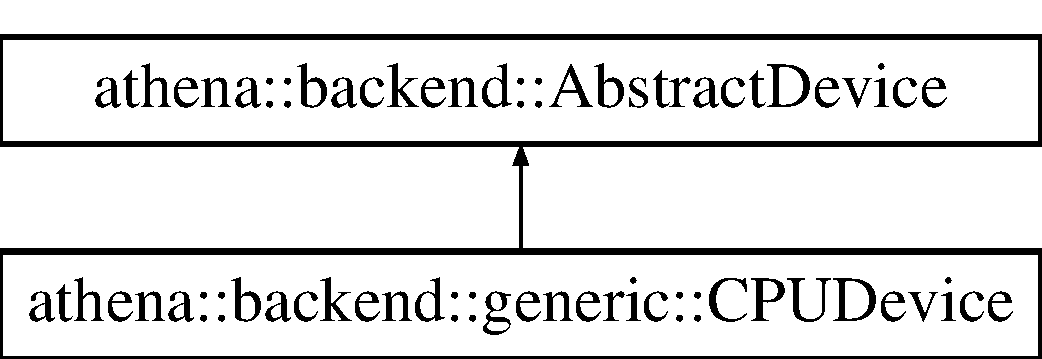
\includegraphics[height=2.000000cm]{dc/dc2/classathena_1_1backend_1_1_abstract_device}
\end{center}
\end{figure}
\subsection*{Public Member Functions}
\begin{DoxyCompactItemize}
\item 
\mbox{\Hypertarget{classathena_1_1backend_1_1_abstract_device_a636bacaa5fc15731e3d5450c2fa56524}\label{classathena_1_1backend_1_1_abstract_device_a636bacaa5fc15731e3d5450c2fa56524}} 
unsigned long {\bfseries get\+Max\+Thread\+Mem\+Size} ()
\item 
\mbox{\Hypertarget{classathena_1_1backend_1_1_abstract_device_a890a1711ae7203de704a2b223adddccc}\label{classathena_1_1backend_1_1_abstract_device_a890a1711ae7203de704a2b223adddccc}} 
void {\bfseries set\+Max\+Thread\+Mem\+Size} (unsigned long size=0)
\item 
\mbox{\Hypertarget{classathena_1_1backend_1_1_abstract_device_aa3c928fe7cfa24e484131dcfffd3c106}\label{classathena_1_1backend_1_1_abstract_device_aa3c928fe7cfa24e484131dcfffd3c106}} 
virtual \mbox{\hyperlink{classathena_1_1backend_1_1_abstract_memory_manager}{Abstract\+Memory\+Manager}} $\ast$ {\bfseries get\+Memory\+Manager} ()=0
\end{DoxyCompactItemize}
\subsection*{Protected Attributes}
\begin{DoxyCompactItemize}
\item 
\mbox{\Hypertarget{classathena_1_1backend_1_1_abstract_device_ac7851210f55e2f709b4ccbd23d9d3f76}\label{classathena_1_1backend_1_1_abstract_device_ac7851210f55e2f709b4ccbd23d9d3f76}} 
unsigned long {\bfseries max\+Thread\+Memory\+Size}
\item 
\mbox{\Hypertarget{classathena_1_1backend_1_1_abstract_device_ade6690f678a25a634104dca162def5f9}\label{classathena_1_1backend_1_1_abstract_device_ade6690f678a25a634104dca162def5f9}} 
unsigned long {\bfseries max\+Threads}
\item 
\mbox{\Hypertarget{classathena_1_1backend_1_1_abstract_device_af689d59af9dbf67df30275ab087b006a}\label{classathena_1_1backend_1_1_abstract_device_af689d59af9dbf67df30275ab087b006a}} 
unsigned long {\bfseries memory\+Size}
\end{DoxyCompactItemize}


\subsection{Detailed Description}


Definition at line 11 of file Abstract\+Device.\+h.



The documentation for this class was generated from the following files\+:\begin{DoxyCompactItemize}
\item 
backend/Abstract\+Device.\+h\item 
backend/Abstract\+Device.\+cpp\end{DoxyCompactItemize}

\hypertarget{classathena_1_1backend_1_1_abstract_executor}{}\section{athena\+:\+:backend\+:\+:Abstract\+Executor Class Reference}
\label{classathena_1_1backend_1_1_abstract_executor}\index{athena\+::backend\+::\+Abstract\+Executor@{athena\+::backend\+::\+Abstract\+Executor}}


{\ttfamily \#include $<$Abstract\+Executor.\+h$>$}

Inheritance diagram for athena\+:\+:backend\+:\+:Abstract\+Executor\+:\begin{figure}[H]
\begin{center}
\leavevmode
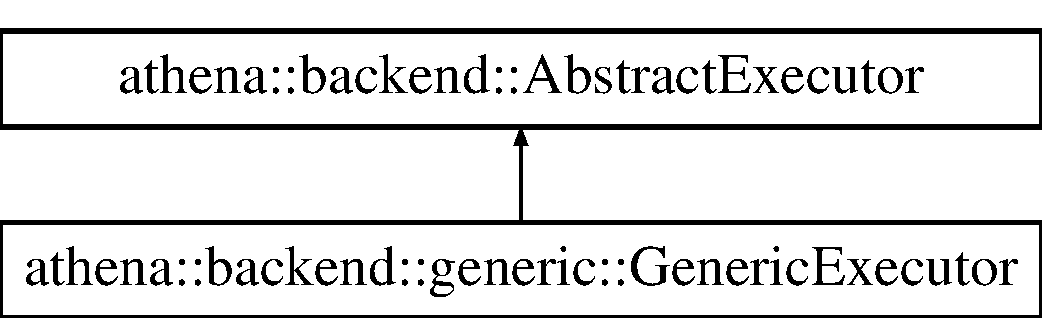
\includegraphics[height=2.000000cm]{d5/d1e/classathena_1_1backend_1_1_abstract_executor}
\end{center}
\end{figure}
\subsection*{Public Member Functions}
\begin{DoxyCompactItemize}
\item 
virtual void \mbox{\hyperlink{classathena_1_1backend_1_1_abstract_executor_a5f179146ae76002b678a4862553f87ce}{execute}} ()=0
\item 
virtual \mbox{\hyperlink{classathena_1_1backend_1_1_abstract_memory_manager}{Abstract\+Memory\+Manager}} $\ast$ \mbox{\hyperlink{classathena_1_1backend_1_1_abstract_executor_a6d61486e2a06500c9c0aa1e03a475e4a}{get\+Memory\+Manager}} ()=0
\item 
void \mbox{\hyperlink{classathena_1_1backend_1_1_abstract_executor_afa06d9875ee6c53986873f29db380893}{set\+Bytecode}} (std\+::vector$<$ vm\+\_\+word $>$ \&bytecode)
\end{DoxyCompactItemize}
\subsection*{Protected Attributes}
\begin{DoxyCompactItemize}
\item 
\mbox{\Hypertarget{classathena_1_1backend_1_1_abstract_executor_a948d95ced27de4fb3445ef341a4b9035}\label{classathena_1_1backend_1_1_abstract_executor_a948d95ced27de4fb3445ef341a4b9035}} 
std\+::vector$<$ vm\+\_\+word $>$ {\bfseries bytecode}
\end{DoxyCompactItemize}


\subsection{Detailed Description}
An Executor is a Virtual Machine that runs Athena \href{https://athenaframework.ml/athena/bytecode/basics.html}{\tt bytecode}. \mbox{\hyperlink{classathena_1_1backend_1_1_abstract_executor}{Abstract\+Executor}} is the base class for all executors. 

Definition at line 18 of file Abstract\+Executor.\+h.



\subsection{Member Function Documentation}
\mbox{\Hypertarget{classathena_1_1backend_1_1_abstract_executor_a5f179146ae76002b678a4862553f87ce}\label{classathena_1_1backend_1_1_abstract_executor_a5f179146ae76002b678a4862553f87ce}} 
\index{athena\+::backend\+::\+Abstract\+Executor@{athena\+::backend\+::\+Abstract\+Executor}!execute@{execute}}
\index{execute@{execute}!athena\+::backend\+::\+Abstract\+Executor@{athena\+::backend\+::\+Abstract\+Executor}}
\subsubsection{\texorpdfstring{execute()}{execute()}}
{\footnotesize\ttfamily virtual void athena\+::backend\+::\+Abstract\+Executor\+::execute (\begin{DoxyParamCaption}{ }\end{DoxyParamCaption})\hspace{0.3cm}{\ttfamily [pure virtual]}}

Executes current bytecode. After execution threads state must be reset. However, memory state (Memory manager and its data) must persist. 

Implemented in \mbox{\hyperlink{classathena_1_1backend_1_1generic_1_1_generic_executor_a38b56c284050d31198b28fcb6595bc73}{athena\+::backend\+::generic\+::\+Generic\+Executor}}.

\mbox{\Hypertarget{classathena_1_1backend_1_1_abstract_executor_a6d61486e2a06500c9c0aa1e03a475e4a}\label{classathena_1_1backend_1_1_abstract_executor_a6d61486e2a06500c9c0aa1e03a475e4a}} 
\index{athena\+::backend\+::\+Abstract\+Executor@{athena\+::backend\+::\+Abstract\+Executor}!get\+Memory\+Manager@{get\+Memory\+Manager}}
\index{get\+Memory\+Manager@{get\+Memory\+Manager}!athena\+::backend\+::\+Abstract\+Executor@{athena\+::backend\+::\+Abstract\+Executor}}
\subsubsection{\texorpdfstring{get\+Memory\+Manager()}{getMemoryManager()}}
{\footnotesize\ttfamily virtual \mbox{\hyperlink{classathena_1_1backend_1_1_abstract_memory_manager}{Abstract\+Memory\+Manager}}$\ast$ athena\+::backend\+::\+Abstract\+Executor\+::get\+Memory\+Manager (\begin{DoxyParamCaption}{ }\end{DoxyParamCaption})\hspace{0.3cm}{\ttfamily [pure virtual]}}

\begin{DoxyReturn}{Returns}
Memory Manager for current device 
\end{DoxyReturn}


Implemented in \mbox{\hyperlink{classathena_1_1backend_1_1generic_1_1_generic_executor_a0560a1dfc0c70ebef0b5be26bb82b9c5}{athena\+::backend\+::generic\+::\+Generic\+Executor}}.

\mbox{\Hypertarget{classathena_1_1backend_1_1_abstract_executor_afa06d9875ee6c53986873f29db380893}\label{classathena_1_1backend_1_1_abstract_executor_afa06d9875ee6c53986873f29db380893}} 
\index{athena\+::backend\+::\+Abstract\+Executor@{athena\+::backend\+::\+Abstract\+Executor}!set\+Bytecode@{set\+Bytecode}}
\index{set\+Bytecode@{set\+Bytecode}!athena\+::backend\+::\+Abstract\+Executor@{athena\+::backend\+::\+Abstract\+Executor}}
\subsubsection{\texorpdfstring{set\+Bytecode()}{setBytecode()}}
{\footnotesize\ttfamily void athena\+::backend\+::\+Abstract\+Executor\+::set\+Bytecode (\begin{DoxyParamCaption}\item[{std\+::vector$<$ vm\+\_\+word $>$ \&}]{bytecode }\end{DoxyParamCaption})}

Sets new bytecode 
\begin{DoxyParams}{Parameters}
{\em bytecode} & Bytecode \\
\hline
\end{DoxyParams}


Definition at line 7 of file Abstract\+Executor.\+cpp.



The documentation for this class was generated from the following files\+:\begin{DoxyCompactItemize}
\item 
backend/Abstract\+Executor.\+h\item 
backend/Abstract\+Executor.\+cpp\end{DoxyCompactItemize}

\hypertarget{classathena_1_1core_1_1loss_1_1_abstract_loss_function}{}\section{athena\+:\+:core\+:\+:loss\+:\+:Abstract\+Loss\+Function Class Reference}
\label{classathena_1_1core_1_1loss_1_1_abstract_loss_function}\index{athena\+::core\+::loss\+::\+Abstract\+Loss\+Function@{athena\+::core\+::loss\+::\+Abstract\+Loss\+Function}}
Inheritance diagram for athena\+:\+:core\+:\+:loss\+:\+:Abstract\+Loss\+Function\+:\begin{figure}[H]
\begin{center}
\leavevmode
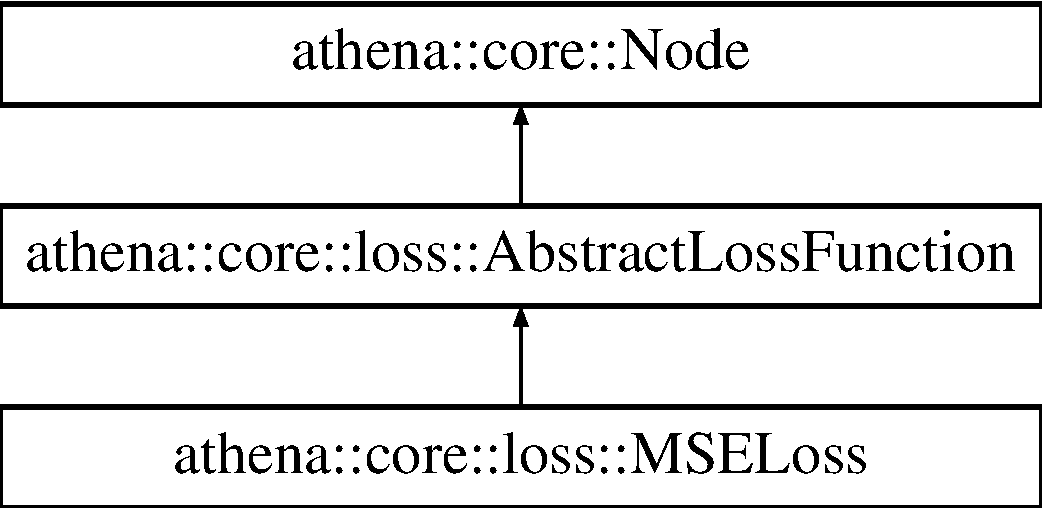
\includegraphics[height=3.000000cm]{classathena_1_1core_1_1loss_1_1_abstract_loss_function}
\end{center}
\end{figure}
\subsection*{Public Member Functions}
\begin{DoxyCompactItemize}
\item 
\mbox{\Hypertarget{classathena_1_1core_1_1loss_1_1_abstract_loss_function_afdb95a15043e5b1951417e6453edd539}\label{classathena_1_1core_1_1loss_1_1_abstract_loss_function_afdb95a15043e5b1951417e6453edd539}} 
{\bfseries Abstract\+Loss\+Function} (\mbox{\hyperlink{classathena_1_1core_1_1_op_kernel}{Op\+Kernel}} $\ast$)
\end{DoxyCompactItemize}
\subsection*{Additional Inherited Members}


The documentation for this class was generated from the following files\+:\begin{DoxyCompactItemize}
\item 
core/loss/Abstract\+Loss\+Function.\+h\item 
core/loss/Abstract\+Loss\+Function.\+cpp\end{DoxyCompactItemize}

\hypertarget{classathena_1_1backend_1_1_abstract_memory_manager}{}\section{athena\+:\+:backend\+:\+:Abstract\+Memory\+Manager Class Reference}
\label{classathena_1_1backend_1_1_abstract_memory_manager}\index{athena\+::backend\+::\+Abstract\+Memory\+Manager@{athena\+::backend\+::\+Abstract\+Memory\+Manager}}


{\ttfamily \#include $<$Abstract\+Memory\+Manager.\+h$>$}

Inheritance diagram for athena\+:\+:backend\+:\+:Abstract\+Memory\+Manager\+:\begin{figure}[H]
\begin{center}
\leavevmode
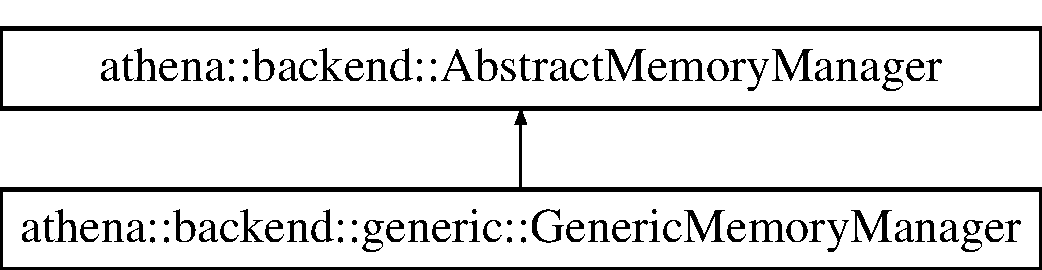
\includegraphics[height=2.000000cm]{d2/df1/classathena_1_1backend_1_1_abstract_memory_manager}
\end{center}
\end{figure}
\subsection*{Public Member Functions}
\begin{DoxyCompactItemize}
\item 
\mbox{\Hypertarget{classathena_1_1backend_1_1_abstract_memory_manager_aecbd824ce1897bc4fabd0280ed11e659}\label{classathena_1_1backend_1_1_abstract_memory_manager_aecbd824ce1897bc4fabd0280ed11e659}} 
virtual void {\bfseries init} ()=0
\item 
\mbox{\Hypertarget{classathena_1_1backend_1_1_abstract_memory_manager_aec0839b1b9bca9c59ea4caed4973888e}\label{classathena_1_1backend_1_1_abstract_memory_manager_aec0839b1b9bca9c59ea4caed4973888e}} 
virtual void {\bfseries deinit} ()=0
\item 
void \mbox{\hyperlink{classathena_1_1backend_1_1_abstract_memory_manager_a358f614d4358f5dce28f17dba6917b1f}{reset\+Table}} ()
\item 
void \mbox{\hyperlink{classathena_1_1backend_1_1_abstract_memory_manager_adaa80b617f6f3f19ba5b1ddd2b0377e7}{add\+Tensor}} (\mbox{\hyperlink{classathena_1_1core_1_1_tensor}{athena\+::core\+::\+Tensor}} $\ast$tensor)
\item 
virtual void $\ast$ \mbox{\hyperlink{classathena_1_1backend_1_1_abstract_memory_manager_ad441d7a2281f5f2b2627272d136f72b8}{get\+Physical\+Address}} (vm\+\_\+word virtual\+Address)=0
\item 
void \mbox{\hyperlink{classathena_1_1backend_1_1_abstract_memory_manager_a2bbfba2a5104aab3068d46214a6ae7df}{load\+And\+Lock}} (\mbox{\hyperlink{classathena_1_1core_1_1_tensor}{athena\+::core\+::\+Tensor}} $\ast$tensor)
\item 
void \mbox{\hyperlink{classathena_1_1backend_1_1_abstract_memory_manager_a47ea5a77f81f91f803f748720c5c19b5}{load\+And\+Lock}} (vm\+\_\+word address)
\item 
virtual void \mbox{\hyperlink{classathena_1_1backend_1_1_abstract_memory_manager_a9fe52e4020802d6f526fba06adce8407}{load\+And\+Lock}} (vm\+\_\+word address, unsigned long length)=0
\item 
virtual void \mbox{\hyperlink{classathena_1_1backend_1_1_abstract_memory_manager_aec859ee3bf6011d8710b2ec4bfc2373e}{unlock}} (vm\+\_\+word address)=0
\item 
virtual void \mbox{\hyperlink{classathena_1_1backend_1_1_abstract_memory_manager_a8ffd6cf21559978f394e2e11815506b5}{delete\+From\+Mem}} (vm\+\_\+word address)=0
\item 
\mbox{\Hypertarget{classathena_1_1backend_1_1_abstract_memory_manager_abd79e10b1e4d51ed592075138e0076f2}\label{classathena_1_1backend_1_1_abstract_memory_manager_abd79e10b1e4d51ed592075138e0076f2}} 
\mbox{\hyperlink{classathena_1_1core_1_1_tensor}{athena\+::core\+::\+Tensor}} $\ast$ {\bfseries get\+Tensor} (vm\+\_\+word address)
\item 
void \mbox{\hyperlink{classathena_1_1backend_1_1_abstract_memory_manager_ad40a653a8b32410956ba835ca1bb3e5f}{allocate\+And\+Lock}} (\mbox{\hyperlink{classathena_1_1core_1_1_tensor}{athena\+::core\+::\+Tensor}} $\ast$tensor)
\item 
void \mbox{\hyperlink{classathena_1_1backend_1_1_abstract_memory_manager_ab5305b3d1ab91960bf179ce0be166120}{allocate\+And\+Lock}} (vm\+\_\+word address)
\item 
virtual void \mbox{\hyperlink{classathena_1_1backend_1_1_abstract_memory_manager_a1b80008e94c21d5ac87f9a45d3f212a8}{allocate\+And\+Lock}} (vm\+\_\+word address, unsigned long length)=0
\item 
virtual void \mbox{\hyperlink{classathena_1_1backend_1_1_abstract_memory_manager_a18562c6f336ff0f7ff800f877696c851}{set\+Data}} (vm\+\_\+word tensor\+Address, vm\+\_\+word offset, vm\+\_\+word length, void $\ast$data)=0
\end{DoxyCompactItemize}
\subsection*{Protected Attributes}
\begin{DoxyCompactItemize}
\item 
\mbox{\Hypertarget{classathena_1_1backend_1_1_abstract_memory_manager_a95e7f8064dea9c79d8e88d39affafda7}\label{classathena_1_1backend_1_1_abstract_memory_manager_a95e7f8064dea9c79d8e88d39affafda7}} 
std\+::list$<$ \mbox{\hyperlink{classathena_1_1core_1_1_tensor}{athena\+::core\+::\+Tensor}} $\ast$$>$ {\bfseries tensors}
\end{DoxyCompactItemize}


\subsection{Detailed Description}
This class is an interface for physical memory managers. They provide conversion between virtual addresses and physical ones. A typical strategy for memory manager is to allocate as much memory as possible and then provide tensors with it. This class also encapsulates table of \mbox{\hyperlink{classathena_1_1core_1_1_tensor}{athena\+::core\+::\+Tensor}} objects. One can think of it as of variables table in a compiler. 

Definition at line 21 of file Abstract\+Memory\+Manager.\+h.



\subsection{Member Function Documentation}
\mbox{\Hypertarget{classathena_1_1backend_1_1_abstract_memory_manager_adaa80b617f6f3f19ba5b1ddd2b0377e7}\label{classathena_1_1backend_1_1_abstract_memory_manager_adaa80b617f6f3f19ba5b1ddd2b0377e7}} 
\index{athena\+::backend\+::\+Abstract\+Memory\+Manager@{athena\+::backend\+::\+Abstract\+Memory\+Manager}!add\+Tensor@{add\+Tensor}}
\index{add\+Tensor@{add\+Tensor}!athena\+::backend\+::\+Abstract\+Memory\+Manager@{athena\+::backend\+::\+Abstract\+Memory\+Manager}}
\subsubsection{\texorpdfstring{add\+Tensor()}{addTensor()}}
{\footnotesize\ttfamily void athena\+::backend\+::\+Abstract\+Memory\+Manager\+::add\+Tensor (\begin{DoxyParamCaption}\item[{\mbox{\hyperlink{classathena_1_1core_1_1_tensor}{athena\+::core\+::\+Tensor}} $\ast$}]{tensor }\end{DoxyParamCaption})}

Adds Tensor to table 
\begin{DoxyParams}{Parameters}
{\em tensor} & Tensor, that will be added \\
\hline
\end{DoxyParams}


Definition at line 11 of file Abstract\+Memory\+Manager.\+cpp.

\mbox{\Hypertarget{classathena_1_1backend_1_1_abstract_memory_manager_ad40a653a8b32410956ba835ca1bb3e5f}\label{classathena_1_1backend_1_1_abstract_memory_manager_ad40a653a8b32410956ba835ca1bb3e5f}} 
\index{athena\+::backend\+::\+Abstract\+Memory\+Manager@{athena\+::backend\+::\+Abstract\+Memory\+Manager}!allocate\+And\+Lock@{allocate\+And\+Lock}}
\index{allocate\+And\+Lock@{allocate\+And\+Lock}!athena\+::backend\+::\+Abstract\+Memory\+Manager@{athena\+::backend\+::\+Abstract\+Memory\+Manager}}
\subsubsection{\texorpdfstring{allocate\+And\+Lock()}{allocateAndLock()}\hspace{0.1cm}{\footnotesize\ttfamily [1/3]}}
{\footnotesize\ttfamily void athena\+::backend\+::\+Abstract\+Memory\+Manager\+::allocate\+And\+Lock (\begin{DoxyParamCaption}\item[{\mbox{\hyperlink{classathena_1_1core_1_1_tensor}{athena\+::core\+::\+Tensor}} $\ast$}]{tensor }\end{DoxyParamCaption})}

Allocate space in the fastest memory available without loading any data and lock it (prevent from being offloaded) 
\begin{DoxyParams}{Parameters}
{\em tensor} & Tensor memory is being allocated for \\
\hline
\end{DoxyParams}


Definition at line 45 of file Abstract\+Memory\+Manager.\+cpp.



Referenced by athena\+::core\+::initializers\+::\+Data\+Initializer\+::initialize().

\mbox{\Hypertarget{classathena_1_1backend_1_1_abstract_memory_manager_ab5305b3d1ab91960bf179ce0be166120}\label{classathena_1_1backend_1_1_abstract_memory_manager_ab5305b3d1ab91960bf179ce0be166120}} 
\index{athena\+::backend\+::\+Abstract\+Memory\+Manager@{athena\+::backend\+::\+Abstract\+Memory\+Manager}!allocate\+And\+Lock@{allocate\+And\+Lock}}
\index{allocate\+And\+Lock@{allocate\+And\+Lock}!athena\+::backend\+::\+Abstract\+Memory\+Manager@{athena\+::backend\+::\+Abstract\+Memory\+Manager}}
\subsubsection{\texorpdfstring{allocate\+And\+Lock()}{allocateAndLock()}\hspace{0.1cm}{\footnotesize\ttfamily [2/3]}}
{\footnotesize\ttfamily void athena\+::backend\+::\+Abstract\+Memory\+Manager\+::allocate\+And\+Lock (\begin{DoxyParamCaption}\item[{vm\+\_\+word}]{address }\end{DoxyParamCaption})}

Allocate space in the fastest memory available without loading any data and lock it (prevent from being offloaded) 
\begin{DoxyParams}{Parameters}
{\em address} & Virtual address of Tensor memory is being allocated for \\
\hline
\end{DoxyParams}


Definition at line 51 of file Abstract\+Memory\+Manager.\+cpp.

\mbox{\Hypertarget{classathena_1_1backend_1_1_abstract_memory_manager_a1b80008e94c21d5ac87f9a45d3f212a8}\label{classathena_1_1backend_1_1_abstract_memory_manager_a1b80008e94c21d5ac87f9a45d3f212a8}} 
\index{athena\+::backend\+::\+Abstract\+Memory\+Manager@{athena\+::backend\+::\+Abstract\+Memory\+Manager}!allocate\+And\+Lock@{allocate\+And\+Lock}}
\index{allocate\+And\+Lock@{allocate\+And\+Lock}!athena\+::backend\+::\+Abstract\+Memory\+Manager@{athena\+::backend\+::\+Abstract\+Memory\+Manager}}
\subsubsection{\texorpdfstring{allocate\+And\+Lock()}{allocateAndLock()}\hspace{0.1cm}{\footnotesize\ttfamily [3/3]}}
{\footnotesize\ttfamily virtual void athena\+::backend\+::\+Abstract\+Memory\+Manager\+::allocate\+And\+Lock (\begin{DoxyParamCaption}\item[{vm\+\_\+word}]{address,  }\item[{unsigned long}]{length }\end{DoxyParamCaption})\hspace{0.3cm}{\ttfamily [pure virtual]}}

Allocate space in the fastest memory available without loading any data and lock it (prevent from being offloaded) 
\begin{DoxyParams}{Parameters}
{\em address} & Virtual address of Tensor memory is being allocated for \\
\hline
{\em length} & Length in bytes for the piece of memory that is being allocated \\
\hline
\end{DoxyParams}


Implemented in \mbox{\hyperlink{classathena_1_1backend_1_1generic_1_1_generic_memory_manager_abe837ac5e3bb60c9bc24836788cae679}{athena\+::backend\+::generic\+::\+Generic\+Memory\+Manager}}.

\mbox{\Hypertarget{classathena_1_1backend_1_1_abstract_memory_manager_a8ffd6cf21559978f394e2e11815506b5}\label{classathena_1_1backend_1_1_abstract_memory_manager_a8ffd6cf21559978f394e2e11815506b5}} 
\index{athena\+::backend\+::\+Abstract\+Memory\+Manager@{athena\+::backend\+::\+Abstract\+Memory\+Manager}!delete\+From\+Mem@{delete\+From\+Mem}}
\index{delete\+From\+Mem@{delete\+From\+Mem}!athena\+::backend\+::\+Abstract\+Memory\+Manager@{athena\+::backend\+::\+Abstract\+Memory\+Manager}}
\subsubsection{\texorpdfstring{delete\+From\+Mem()}{deleteFromMem()}}
{\footnotesize\ttfamily virtual void athena\+::backend\+::\+Abstract\+Memory\+Manager\+::delete\+From\+Mem (\begin{DoxyParamCaption}\item[{vm\+\_\+word}]{address }\end{DoxyParamCaption})\hspace{0.3cm}{\ttfamily [pure virtual]}}

Mark corresponding memory chunk as free 
\begin{DoxyParams}{Parameters}
{\em address} & Virtual address \\
\hline
\end{DoxyParams}


Implemented in \mbox{\hyperlink{classathena_1_1backend_1_1generic_1_1_generic_memory_manager_a2767b6c1f5887a2928b665e0c1b454c7}{athena\+::backend\+::generic\+::\+Generic\+Memory\+Manager}}.

\mbox{\Hypertarget{classathena_1_1backend_1_1_abstract_memory_manager_ad441d7a2281f5f2b2627272d136f72b8}\label{classathena_1_1backend_1_1_abstract_memory_manager_ad441d7a2281f5f2b2627272d136f72b8}} 
\index{athena\+::backend\+::\+Abstract\+Memory\+Manager@{athena\+::backend\+::\+Abstract\+Memory\+Manager}!get\+Physical\+Address@{get\+Physical\+Address}}
\index{get\+Physical\+Address@{get\+Physical\+Address}!athena\+::backend\+::\+Abstract\+Memory\+Manager@{athena\+::backend\+::\+Abstract\+Memory\+Manager}}
\subsubsection{\texorpdfstring{get\+Physical\+Address()}{getPhysicalAddress()}}
{\footnotesize\ttfamily virtual void$\ast$ athena\+::backend\+::\+Abstract\+Memory\+Manager\+::get\+Physical\+Address (\begin{DoxyParamCaption}\item[{vm\+\_\+word}]{virtual\+Address }\end{DoxyParamCaption})\hspace{0.3cm}{\ttfamily [pure virtual]}}

Convert virtual address to physical one 
\begin{DoxyParams}{Parameters}
{\em virtual\+Address} & Virtual address, unsigned long from 0 to 2$^\wedge$64-\/1 \\
\hline
\end{DoxyParams}
\begin{DoxyReturn}{Returns}
Pointer to physical memory 
\end{DoxyReturn}


Implemented in \mbox{\hyperlink{classathena_1_1backend_1_1generic_1_1_generic_memory_manager_a7f3dacb56bd95b837910441d0aef1dd8}{athena\+::backend\+::generic\+::\+Generic\+Memory\+Manager}}.

\mbox{\Hypertarget{classathena_1_1backend_1_1_abstract_memory_manager_a2bbfba2a5104aab3068d46214a6ae7df}\label{classathena_1_1backend_1_1_abstract_memory_manager_a2bbfba2a5104aab3068d46214a6ae7df}} 
\index{athena\+::backend\+::\+Abstract\+Memory\+Manager@{athena\+::backend\+::\+Abstract\+Memory\+Manager}!load\+And\+Lock@{load\+And\+Lock}}
\index{load\+And\+Lock@{load\+And\+Lock}!athena\+::backend\+::\+Abstract\+Memory\+Manager@{athena\+::backend\+::\+Abstract\+Memory\+Manager}}
\subsubsection{\texorpdfstring{load\+And\+Lock()}{loadAndLock()}\hspace{0.1cm}{\footnotesize\ttfamily [1/3]}}
{\footnotesize\ttfamily void athena\+::backend\+::\+Abstract\+Memory\+Manager\+::load\+And\+Lock (\begin{DoxyParamCaption}\item[{\mbox{\hyperlink{classathena_1_1core_1_1_tensor}{athena\+::core\+::\+Tensor}} $\ast$}]{tensor }\end{DoxyParamCaption})}

Move data to the fastest memory type available (e.\+g. from hard drive to R\+AM) and lock it (prevent from being offloaded) 
\begin{DoxyParams}{Parameters}
{\em tensor} & Tensor containing data \\
\hline
\end{DoxyParams}


Definition at line 16 of file Abstract\+Memory\+Manager.\+cpp.

\mbox{\Hypertarget{classathena_1_1backend_1_1_abstract_memory_manager_a47ea5a77f81f91f803f748720c5c19b5}\label{classathena_1_1backend_1_1_abstract_memory_manager_a47ea5a77f81f91f803f748720c5c19b5}} 
\index{athena\+::backend\+::\+Abstract\+Memory\+Manager@{athena\+::backend\+::\+Abstract\+Memory\+Manager}!load\+And\+Lock@{load\+And\+Lock}}
\index{load\+And\+Lock@{load\+And\+Lock}!athena\+::backend\+::\+Abstract\+Memory\+Manager@{athena\+::backend\+::\+Abstract\+Memory\+Manager}}
\subsubsection{\texorpdfstring{load\+And\+Lock()}{loadAndLock()}\hspace{0.1cm}{\footnotesize\ttfamily [2/3]}}
{\footnotesize\ttfamily void athena\+::backend\+::\+Abstract\+Memory\+Manager\+::load\+And\+Lock (\begin{DoxyParamCaption}\item[{vm\+\_\+word}]{address }\end{DoxyParamCaption})}

Move data to the fastest memory type available (e.\+g. from hard drive to R\+AM) and lock it (prevent from being offloaded) 
\begin{DoxyParams}{Parameters}
{\em address} & Virtual address of Tensor containing data \\
\hline
\end{DoxyParams}


Definition at line 21 of file Abstract\+Memory\+Manager.\+cpp.

\mbox{\Hypertarget{classathena_1_1backend_1_1_abstract_memory_manager_a9fe52e4020802d6f526fba06adce8407}\label{classathena_1_1backend_1_1_abstract_memory_manager_a9fe52e4020802d6f526fba06adce8407}} 
\index{athena\+::backend\+::\+Abstract\+Memory\+Manager@{athena\+::backend\+::\+Abstract\+Memory\+Manager}!load\+And\+Lock@{load\+And\+Lock}}
\index{load\+And\+Lock@{load\+And\+Lock}!athena\+::backend\+::\+Abstract\+Memory\+Manager@{athena\+::backend\+::\+Abstract\+Memory\+Manager}}
\subsubsection{\texorpdfstring{load\+And\+Lock()}{loadAndLock()}\hspace{0.1cm}{\footnotesize\ttfamily [3/3]}}
{\footnotesize\ttfamily virtual void athena\+::backend\+::\+Abstract\+Memory\+Manager\+::load\+And\+Lock (\begin{DoxyParamCaption}\item[{vm\+\_\+word}]{address,  }\item[{unsigned long}]{length }\end{DoxyParamCaption})\hspace{0.3cm}{\ttfamily [pure virtual]}}

Move data to the fastest memory type available (e.\+g. from hard drive to R\+AM) and lock it (prevent from being offloaded) 
\begin{DoxyParams}{Parameters}
{\em address} & Virtual address \\
\hline
{\em length} & Size of Tensor in bytes \\
\hline
\end{DoxyParams}


Implemented in \mbox{\hyperlink{classathena_1_1backend_1_1generic_1_1_generic_memory_manager_aa7fce5a6cbd9c4f5ad1868735e4546a8}{athena\+::backend\+::generic\+::\+Generic\+Memory\+Manager}}.

\mbox{\Hypertarget{classathena_1_1backend_1_1_abstract_memory_manager_a358f614d4358f5dce28f17dba6917b1f}\label{classathena_1_1backend_1_1_abstract_memory_manager_a358f614d4358f5dce28f17dba6917b1f}} 
\index{athena\+::backend\+::\+Abstract\+Memory\+Manager@{athena\+::backend\+::\+Abstract\+Memory\+Manager}!reset\+Table@{reset\+Table}}
\index{reset\+Table@{reset\+Table}!athena\+::backend\+::\+Abstract\+Memory\+Manager@{athena\+::backend\+::\+Abstract\+Memory\+Manager}}
\subsubsection{\texorpdfstring{reset\+Table()}{resetTable()}}
{\footnotesize\ttfamily void athena\+::backend\+::\+Abstract\+Memory\+Manager\+::reset\+Table (\begin{DoxyParamCaption}{ }\end{DoxyParamCaption})}

Clears table of Tensors 

Definition at line 7 of file Abstract\+Memory\+Manager.\+cpp.

\mbox{\Hypertarget{classathena_1_1backend_1_1_abstract_memory_manager_a18562c6f336ff0f7ff800f877696c851}\label{classathena_1_1backend_1_1_abstract_memory_manager_a18562c6f336ff0f7ff800f877696c851}} 
\index{athena\+::backend\+::\+Abstract\+Memory\+Manager@{athena\+::backend\+::\+Abstract\+Memory\+Manager}!set\+Data@{set\+Data}}
\index{set\+Data@{set\+Data}!athena\+::backend\+::\+Abstract\+Memory\+Manager@{athena\+::backend\+::\+Abstract\+Memory\+Manager}}
\subsubsection{\texorpdfstring{set\+Data()}{setData()}}
{\footnotesize\ttfamily virtual void athena\+::backend\+::\+Abstract\+Memory\+Manager\+::set\+Data (\begin{DoxyParamCaption}\item[{vm\+\_\+word}]{tensor\+Address,  }\item[{vm\+\_\+word}]{offset,  }\item[{vm\+\_\+word}]{length,  }\item[{void $\ast$}]{data }\end{DoxyParamCaption})\hspace{0.3cm}{\ttfamily [pure virtual]}}

Sets memory with the data 
\begin{DoxyParams}{Parameters}
{\em tensor\+Address} & Virtual address of Tensor beginning (see Tensor\+::get\+Start\+Address) \\
\hline
{\em offset} & Offset in bytes from the beginning \\
\hline
{\em length} & Length of piece of data in bytes \\
\hline
{\em data} & Pointer to data \\
\hline
\end{DoxyParams}


Implemented in \mbox{\hyperlink{classathena_1_1backend_1_1generic_1_1_generic_memory_manager_aa4e2e533d897cf6d042d8a086633bd9d}{athena\+::backend\+::generic\+::\+Generic\+Memory\+Manager}}.



Referenced by athena\+::core\+::initializers\+::\+Data\+Initializer\+::initialize().

\mbox{\Hypertarget{classathena_1_1backend_1_1_abstract_memory_manager_aec859ee3bf6011d8710b2ec4bfc2373e}\label{classathena_1_1backend_1_1_abstract_memory_manager_aec859ee3bf6011d8710b2ec4bfc2373e}} 
\index{athena\+::backend\+::\+Abstract\+Memory\+Manager@{athena\+::backend\+::\+Abstract\+Memory\+Manager}!unlock@{unlock}}
\index{unlock@{unlock}!athena\+::backend\+::\+Abstract\+Memory\+Manager@{athena\+::backend\+::\+Abstract\+Memory\+Manager}}
\subsubsection{\texorpdfstring{unlock()}{unlock()}}
{\footnotesize\ttfamily virtual void athena\+::backend\+::\+Abstract\+Memory\+Manager\+::unlock (\begin{DoxyParamCaption}\item[{vm\+\_\+word}]{address }\end{DoxyParamCaption})\hspace{0.3cm}{\ttfamily [pure virtual]}}

Lets data be offloaded to a slower memory type (e.\+g. from R\+AM to H\+DD) 
\begin{DoxyParams}{Parameters}
{\em address} & Virtual address \\
\hline
\end{DoxyParams}


Implemented in \mbox{\hyperlink{classathena_1_1backend_1_1generic_1_1_generic_memory_manager_a58a2b56a07a96c3cabb7b8fd079b3eae}{athena\+::backend\+::generic\+::\+Generic\+Memory\+Manager}}.



Referenced by athena\+::core\+::initializers\+::\+Data\+Initializer\+::initialize().



The documentation for this class was generated from the following files\+:\begin{DoxyCompactItemize}
\item 
backend/Abstract\+Memory\+Manager.\+h\item 
backend/Abstract\+Memory\+Manager.\+cpp\end{DoxyCompactItemize}

\hypertarget{classathena_1_1core_1_1optimizers_1_1_abstract_optimizer}{}\section{athena\+:\+:core\+:\+:optimizers\+:\+:Abstract\+Optimizer Class Reference}
\label{classathena_1_1core_1_1optimizers_1_1_abstract_optimizer}\index{athena\+::core\+::optimizers\+::\+Abstract\+Optimizer@{athena\+::core\+::optimizers\+::\+Abstract\+Optimizer}}
Inheritance diagram for athena\+:\+:core\+:\+:optimizers\+:\+:Abstract\+Optimizer\+:\begin{figure}[H]
\begin{center}
\leavevmode
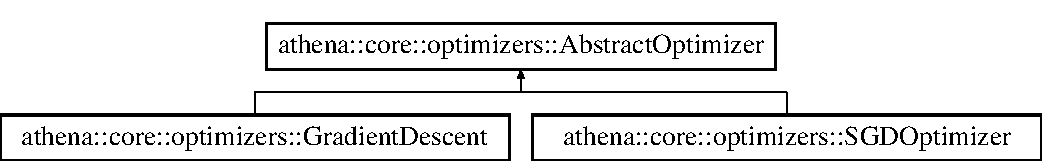
\includegraphics[height=2.000000cm]{d5/d97/classathena_1_1core_1_1optimizers_1_1_abstract_optimizer}
\end{center}
\end{figure}
\subsection*{Public Member Functions}
\begin{DoxyCompactItemize}
\item 
\mbox{\Hypertarget{classathena_1_1core_1_1optimizers_1_1_abstract_optimizer_a87422b9b479a84aa2b882e54e7ba22d5}\label{classathena_1_1core_1_1optimizers_1_1_abstract_optimizer_a87422b9b479a84aa2b882e54e7ba22d5}} 
{\bfseries Abstract\+Optimizer} (\mbox{\hyperlink{classathena_1_1core_1_1loss_1_1_abstract_loss_function}{athena\+::core\+::loss\+::\+Abstract\+Loss\+Function}} $\ast$loss)
\item 
\mbox{\Hypertarget{classathena_1_1core_1_1optimizers_1_1_abstract_optimizer_a4aaf186d6810a25cf54015ba23e0a809}\label{classathena_1_1core_1_1optimizers_1_1_abstract_optimizer_a4aaf186d6810a25cf54015ba23e0a809}} 
void {\bfseries init} (\mbox{\hyperlink{classathena_1_1core_1_1_session}{Session}} $\ast$session)
\item 
\mbox{\Hypertarget{classathena_1_1core_1_1optimizers_1_1_abstract_optimizer_a1131df49e42aff2009ccd22621a6447e}\label{classathena_1_1core_1_1optimizers_1_1_abstract_optimizer_a1131df49e42aff2009ccd22621a6447e}} 
virtual void {\bfseries prepare} ()=0
\item 
\mbox{\Hypertarget{classathena_1_1core_1_1optimizers_1_1_abstract_optimizer_ad0106d7566fd68761a502aa7bff24c68}\label{classathena_1_1core_1_1optimizers_1_1_abstract_optimizer_ad0106d7566fd68761a502aa7bff24c68}} 
virtual void {\bfseries minimize} ()=0
\end{DoxyCompactItemize}
\subsection*{Protected Attributes}
\begin{DoxyCompactItemize}
\item 
\mbox{\Hypertarget{classathena_1_1core_1_1optimizers_1_1_abstract_optimizer_a531c36dd399081caeacfc8974805de79}\label{classathena_1_1core_1_1optimizers_1_1_abstract_optimizer_a531c36dd399081caeacfc8974805de79}} 
std\+::vector$<$ \mbox{\hyperlink{classathena_1_1core_1_1_input_node}{Input\+Node}} $\ast$$>$ {\bfseries head\+Nodes}
\item 
\mbox{\Hypertarget{classathena_1_1core_1_1optimizers_1_1_abstract_optimizer_ad96008b4e5dec5e9bf5ece0cf4fdcba6}\label{classathena_1_1core_1_1optimizers_1_1_abstract_optimizer_ad96008b4e5dec5e9bf5ece0cf4fdcba6}} 
std\+::vector$<$ vm\+\_\+word $>$ {\bfseries bytecode}
\item 
\mbox{\Hypertarget{classathena_1_1core_1_1optimizers_1_1_abstract_optimizer_abd29bf7d7d1f9f553756b918f526e2fc}\label{classathena_1_1core_1_1optimizers_1_1_abstract_optimizer_abd29bf7d7d1f9f553756b918f526e2fc}} 
unsigned long {\bfseries last\+Result\+Cell}
\item 
\mbox{\Hypertarget{classathena_1_1core_1_1optimizers_1_1_abstract_optimizer_a7cc6da9a5944cf7eba19dc04814e478b}\label{classathena_1_1core_1_1optimizers_1_1_abstract_optimizer_a7cc6da9a5944cf7eba19dc04814e478b}} 
\mbox{\hyperlink{classathena_1_1core_1_1_session}{Session}} $\ast$ {\bfseries session}
\item 
\mbox{\Hypertarget{classathena_1_1core_1_1optimizers_1_1_abstract_optimizer_a9043b6609054109d6f590477bd62c975}\label{classathena_1_1core_1_1optimizers_1_1_abstract_optimizer_a9043b6609054109d6f590477bd62c975}} 
\mbox{\hyperlink{classathena_1_1core_1_1loss_1_1_abstract_loss_function}{athena\+::core\+::loss\+::\+Abstract\+Loss\+Function}} $\ast$ {\bfseries loss}
\end{DoxyCompactItemize}


\subsection{Detailed Description}


Definition at line 15 of file Abstract\+Optimizer.\+h.



The documentation for this class was generated from the following files\+:\begin{DoxyCompactItemize}
\item 
core/optimizers/Abstract\+Optimizer.\+h\item 
core/optimizers/Abstract\+Optimizer.\+cpp\end{DoxyCompactItemize}

\hypertarget{classathena_1_1core_1_1kernels_1_1_add_op_kernel}{}\section{athena\+:\+:core\+:\+:kernels\+:\+:Add\+Op\+Kernel Class Reference}
\label{classathena_1_1core_1_1kernels_1_1_add_op_kernel}\index{athena\+::core\+::kernels\+::\+Add\+Op\+Kernel@{athena\+::core\+::kernels\+::\+Add\+Op\+Kernel}}


{\ttfamily \#include $<$Add\+Op\+Kernel.\+h$>$}

Inheritance diagram for athena\+:\+:core\+:\+:kernels\+:\+:Add\+Op\+Kernel\+:\begin{figure}[H]
\begin{center}
\leavevmode
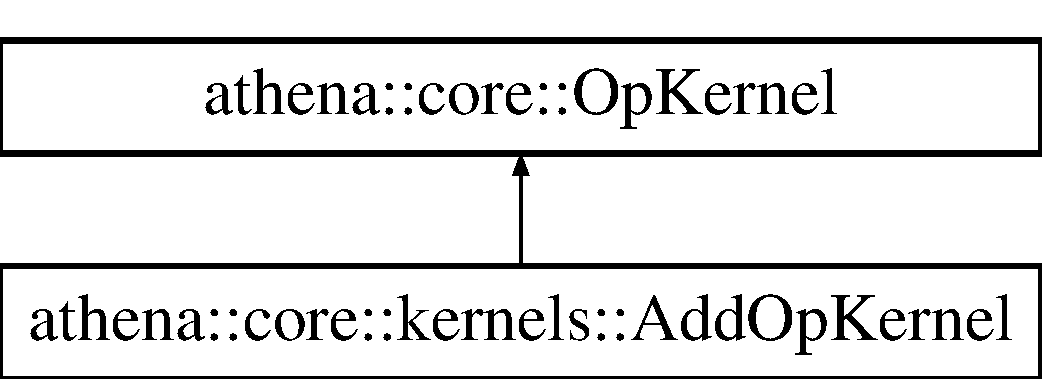
\includegraphics[height=2.000000cm]{classathena_1_1core_1_1kernels_1_1_add_op_kernel}
\end{center}
\end{figure}
\subsection*{Public Member Functions}
\begin{DoxyCompactItemize}
\item 
int \mbox{\hyperlink{classathena_1_1core_1_1kernels_1_1_add_op_kernel_a296a0c69a7b906037324cce2b64827e1}{get\+Operands\+Count}} () override
\item 
\mbox{\hyperlink{classathena_1_1core_1_1_tensor_shape}{athena\+::core\+::\+Tensor\+Shape}} \& \mbox{\hyperlink{classathena_1_1core_1_1kernels_1_1_add_op_kernel_a687d68d7374e9546f01cefcbfb382d04}{get\+Output\+Shape}} (std\+::vector$<$ \mbox{\hyperlink{classathena_1_1core_1_1_tensor_shape}{athena\+::core\+::\+Tensor\+Shape}} $>$ \&shapes) override
\item 
\mbox{\hyperlink{classathena_1_1core_1_1_tensor_shape}{athena\+::core\+::\+Tensor\+Shape}} \& \mbox{\hyperlink{classathena_1_1core_1_1kernels_1_1_add_op_kernel_a240d13047b8fd7676bf1f9d2bc94298f}{get\+Derivative\+Shape}} (int d, std\+::vector$<$ \mbox{\hyperlink{classathena_1_1core_1_1_tensor_shape}{athena\+::core\+::\+Tensor\+Shape}} $>$ \&shapes) override
\item 
\mbox{\Hypertarget{classathena_1_1core_1_1kernels_1_1_add_op_kernel_a6aa2ce3c6d4c2b2eeaf99a83189e1f70}\label{classathena_1_1core_1_1kernels_1_1_add_op_kernel_a6aa2ce3c6d4c2b2eeaf99a83189e1f70}} 
std\+::vector$<$ vm\+\_\+word $>$ {\bfseries get\+Op\+Bytecode} (std\+::vector$<$ vm\+\_\+word $>$ args, vm\+\_\+word result\+Cell) override
\item 
std\+::vector$<$ vm\+\_\+word $>$ \mbox{\hyperlink{classathena_1_1core_1_1kernels_1_1_add_op_kernel_a97ac0c3c61c772563221c3148d553841}{get\+Derivative\+Bytecode}} (int d, std\+::vector$<$ vm\+\_\+word $>$ args, vm\+\_\+word result\+Cell) override
\end{DoxyCompactItemize}
\subsection*{Additional Inherited Members}


\subsection{Detailed Description}
Performs sum of 2 given Tensors 

\subsection{Member Function Documentation}
\mbox{\Hypertarget{classathena_1_1core_1_1kernels_1_1_add_op_kernel_a97ac0c3c61c772563221c3148d553841}\label{classathena_1_1core_1_1kernels_1_1_add_op_kernel_a97ac0c3c61c772563221c3148d553841}} 
\index{athena\+::core\+::kernels\+::\+Add\+Op\+Kernel@{athena\+::core\+::kernels\+::\+Add\+Op\+Kernel}!get\+Derivative\+Bytecode@{get\+Derivative\+Bytecode}}
\index{get\+Derivative\+Bytecode@{get\+Derivative\+Bytecode}!athena\+::core\+::kernels\+::\+Add\+Op\+Kernel@{athena\+::core\+::kernels\+::\+Add\+Op\+Kernel}}
\subsubsection{\texorpdfstring{get\+Derivative\+Bytecode()}{getDerivativeBytecode()}}
{\footnotesize\ttfamily std\+::vector$<$ unsigned long $>$ athena\+::core\+::kernels\+::\+Add\+Op\+Kernel\+::get\+Derivative\+Bytecode (\begin{DoxyParamCaption}\item[{int}]{d,  }\item[{std\+::vector$<$ vm\+\_\+word $>$}]{args,  }\item[{vm\+\_\+word}]{result\+Cell }\end{DoxyParamCaption})\hspace{0.3cm}{\ttfamily [override]}, {\ttfamily [virtual]}}

Generates bytecode to calculate partial derivative 
\begin{DoxyParams}{Parameters}
{\em d} & Number of variable with respect to which derivative is calculated \\
\hline
{\em args} & Function arguments \\
\hline
{\em result\+Cell} & Number of memory cell where results are saved \\
\hline
\end{DoxyParams}
\begin{DoxyReturn}{Returns}

\end{DoxyReturn}


Implements \mbox{\hyperlink{classathena_1_1core_1_1_op_kernel_ad500db1afc5a7c10acff8ecb8f1bee4d}{athena\+::core\+::\+Op\+Kernel}}.

\mbox{\Hypertarget{classathena_1_1core_1_1kernels_1_1_add_op_kernel_a240d13047b8fd7676bf1f9d2bc94298f}\label{classathena_1_1core_1_1kernels_1_1_add_op_kernel_a240d13047b8fd7676bf1f9d2bc94298f}} 
\index{athena\+::core\+::kernels\+::\+Add\+Op\+Kernel@{athena\+::core\+::kernels\+::\+Add\+Op\+Kernel}!get\+Derivative\+Shape@{get\+Derivative\+Shape}}
\index{get\+Derivative\+Shape@{get\+Derivative\+Shape}!athena\+::core\+::kernels\+::\+Add\+Op\+Kernel@{athena\+::core\+::kernels\+::\+Add\+Op\+Kernel}}
\subsubsection{\texorpdfstring{get\+Derivative\+Shape()}{getDerivativeShape()}}
{\footnotesize\ttfamily \mbox{\hyperlink{classathena_1_1core_1_1_tensor_shape}{athena\+::core\+::\+Tensor\+Shape}} \& athena\+::core\+::kernels\+::\+Add\+Op\+Kernel\+::get\+Derivative\+Shape (\begin{DoxyParamCaption}\item[{int}]{d,  }\item[{std\+::vector$<$ \mbox{\hyperlink{classathena_1_1core_1_1_tensor_shape}{athena\+::core\+::\+Tensor\+Shape}} $>$ \&}]{shapes }\end{DoxyParamCaption})\hspace{0.3cm}{\ttfamily [override]}, {\ttfamily [virtual]}}

It is important for some operations to have certain size of their operands 
\begin{DoxyParams}{Parameters}
{\em shape} & Original operand shape \\
\hline
{\em dim} & Dimensionality \\
\hline
\end{DoxyParams}
\begin{DoxyReturn}{Returns}
New shape 
\end{DoxyReturn}


Implements \mbox{\hyperlink{classathena_1_1core_1_1_op_kernel_ad95af6dd184ce7ee9182ec7ca54b6c4d}{athena\+::core\+::\+Op\+Kernel}}.

\mbox{\Hypertarget{classathena_1_1core_1_1kernels_1_1_add_op_kernel_a296a0c69a7b906037324cce2b64827e1}\label{classathena_1_1core_1_1kernels_1_1_add_op_kernel_a296a0c69a7b906037324cce2b64827e1}} 
\index{athena\+::core\+::kernels\+::\+Add\+Op\+Kernel@{athena\+::core\+::kernels\+::\+Add\+Op\+Kernel}!get\+Operands\+Count@{get\+Operands\+Count}}
\index{get\+Operands\+Count@{get\+Operands\+Count}!athena\+::core\+::kernels\+::\+Add\+Op\+Kernel@{athena\+::core\+::kernels\+::\+Add\+Op\+Kernel}}
\subsubsection{\texorpdfstring{get\+Operands\+Count()}{getOperandsCount()}}
{\footnotesize\ttfamily int athena\+::core\+::kernels\+::\+Add\+Op\+Kernel\+::get\+Operands\+Count (\begin{DoxyParamCaption}{ }\end{DoxyParamCaption})\hspace{0.3cm}{\ttfamily [override]}, {\ttfamily [virtual]}}

There can be unary, binary and other operations \begin{DoxyReturn}{Returns}
Number of operands accepted 
\end{DoxyReturn}


Implements \mbox{\hyperlink{classathena_1_1core_1_1_op_kernel_add97d4c132d80ecd9915acfedf7c9119}{athena\+::core\+::\+Op\+Kernel}}.

\mbox{\Hypertarget{classathena_1_1core_1_1kernels_1_1_add_op_kernel_a687d68d7374e9546f01cefcbfb382d04}\label{classathena_1_1core_1_1kernels_1_1_add_op_kernel_a687d68d7374e9546f01cefcbfb382d04}} 
\index{athena\+::core\+::kernels\+::\+Add\+Op\+Kernel@{athena\+::core\+::kernels\+::\+Add\+Op\+Kernel}!get\+Output\+Shape@{get\+Output\+Shape}}
\index{get\+Output\+Shape@{get\+Output\+Shape}!athena\+::core\+::kernels\+::\+Add\+Op\+Kernel@{athena\+::core\+::kernels\+::\+Add\+Op\+Kernel}}
\subsubsection{\texorpdfstring{get\+Output\+Shape()}{getOutputShape()}}
{\footnotesize\ttfamily \mbox{\hyperlink{classathena_1_1core_1_1_tensor_shape}{athena\+::core\+::\+Tensor\+Shape}} \& athena\+::core\+::kernels\+::\+Add\+Op\+Kernel\+::get\+Output\+Shape (\begin{DoxyParamCaption}\item[{std\+::vector$<$ \mbox{\hyperlink{classathena_1_1core_1_1_tensor_shape}{athena\+::core\+::\+Tensor\+Shape}} $>$ \&}]{shapes }\end{DoxyParamCaption})\hspace{0.3cm}{\ttfamily [override]}, {\ttfamily [virtual]}}

It is important for some operations to have certain size of their operands 
\begin{DoxyParams}{Parameters}
{\em shape} & Original operand shape \\
\hline
{\em dim} & Dimensionality \\
\hline
\end{DoxyParams}
\begin{DoxyReturn}{Returns}
New shape 
\end{DoxyReturn}


Implements \mbox{\hyperlink{classathena_1_1core_1_1_op_kernel_a762e541463ffd089b47a8e6755c30fe1}{athena\+::core\+::\+Op\+Kernel}}.



The documentation for this class was generated from the following files\+:\begin{DoxyCompactItemize}
\item 
core/kernels/Add\+Op\+Kernel.\+h\item 
core/kernels/Add\+Op\+Kernel.\+cpp\end{DoxyCompactItemize}

\hypertarget{classathena_1_1backend_1_1generic_1_1_c_p_u_device}{}\section{athena\+:\+:backend\+:\+:generic\+:\+:C\+P\+U\+Device Class Reference}
\label{classathena_1_1backend_1_1generic_1_1_c_p_u_device}\index{athena\+::backend\+::generic\+::\+C\+P\+U\+Device@{athena\+::backend\+::generic\+::\+C\+P\+U\+Device}}


{\ttfamily \#include $<$C\+P\+U\+Device.\+h$>$}

Inheritance diagram for athena\+:\+:backend\+:\+:generic\+:\+:C\+P\+U\+Device\+:\begin{figure}[H]
\begin{center}
\leavevmode
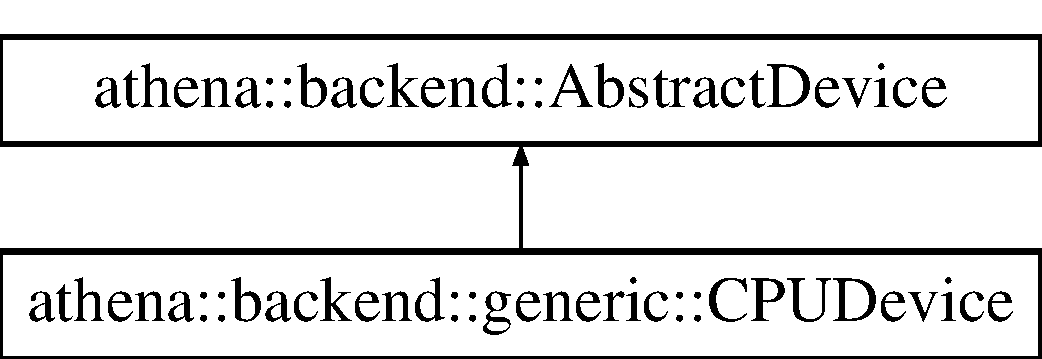
\includegraphics[height=2.000000cm]{db/d7b/classathena_1_1backend_1_1generic_1_1_c_p_u_device}
\end{center}
\end{figure}
\subsection*{Public Member Functions}
\begin{DoxyCompactItemize}
\item 
\mbox{\Hypertarget{classathena_1_1backend_1_1generic_1_1_c_p_u_device_a813561ea04e66b4fc25c720242c70238}\label{classathena_1_1backend_1_1generic_1_1_c_p_u_device_a813561ea04e66b4fc25c720242c70238}} 
\mbox{\hyperlink{classathena_1_1backend_1_1_abstract_memory_manager}{Abstract\+Memory\+Manager}} $\ast$ {\bfseries get\+Memory\+Manager} () override
\end{DoxyCompactItemize}
\subsection*{Additional Inherited Members}


\subsection{Detailed Description}
This class represents a C\+PU It encapsulates Memory Manager 

Definition at line 18 of file C\+P\+U\+Device.\+h.



The documentation for this class was generated from the following files\+:\begin{DoxyCompactItemize}
\item 
backend/generic/C\+P\+U\+Device.\+h\item 
backend/generic/C\+P\+U\+Device.\+cpp\end{DoxyCompactItemize}

\hypertarget{classathena_1_1backend_1_1generic_1_1_generic_executor}{}\section{athena\+:\+:backend\+:\+:generic\+:\+:Generic\+Executor Class Reference}
\label{classathena_1_1backend_1_1generic_1_1_generic_executor}\index{athena\+::backend\+::generic\+::\+Generic\+Executor@{athena\+::backend\+::generic\+::\+Generic\+Executor}}
Inheritance diagram for athena\+:\+:backend\+:\+:generic\+:\+:Generic\+Executor\+:\begin{figure}[H]
\begin{center}
\leavevmode
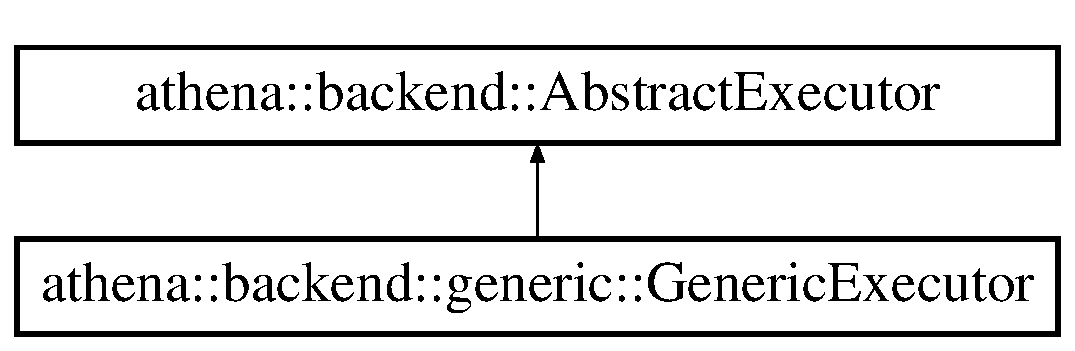
\includegraphics[height=2.000000cm]{classathena_1_1backend_1_1generic_1_1_generic_executor}
\end{center}
\end{figure}
\subsection*{Public Member Functions}
\begin{DoxyCompactItemize}
\item 
\mbox{\Hypertarget{classathena_1_1backend_1_1generic_1_1_generic_executor_a150867180e469045e4dc9cbbce8e2774}\label{classathena_1_1backend_1_1generic_1_1_generic_executor_a150867180e469045e4dc9cbbce8e2774}} 
{\bfseries Generic\+Executor} (std\+::vector$<$ vm\+\_\+word $>$ \&bytecode, unsigned long max\+Mem, \mbox{\hyperlink{classathena_1_1backend_1_1generic_1_1_c_p_u_device}{C\+P\+U\+Device}} $\ast$cpu\+Device)
\item 
\mbox{\Hypertarget{classathena_1_1backend_1_1generic_1_1_generic_executor_a38b56c284050d31198b28fcb6595bc73}\label{classathena_1_1backend_1_1generic_1_1_generic_executor_a38b56c284050d31198b28fcb6595bc73}} 
void {\bfseries execute} () override
\item 
\mbox{\Hypertarget{classathena_1_1backend_1_1generic_1_1_generic_executor_a0560a1dfc0c70ebef0b5be26bb82b9c5}\label{classathena_1_1backend_1_1generic_1_1_generic_executor_a0560a1dfc0c70ebef0b5be26bb82b9c5}} 
\mbox{\hyperlink{classathena_1_1backend_1_1_abstract_memory_manager}{Abstract\+Memory\+Manager}} $\ast$ {\bfseries get\+Memory\+Manager} () override
\end{DoxyCompactItemize}


The documentation for this class was generated from the following files\+:\begin{DoxyCompactItemize}
\item 
backend/generic/Generic\+Executor.\+h\item 
backend/generic/Generic\+Executor.\+cpp\end{DoxyCompactItemize}

\hypertarget{classathena_1_1backend_1_1generic_1_1_generic_memory_manager}{}\section{athena\+:\+:backend\+:\+:generic\+:\+:Generic\+Memory\+Manager Class Reference}
\label{classathena_1_1backend_1_1generic_1_1_generic_memory_manager}\index{athena\+::backend\+::generic\+::\+Generic\+Memory\+Manager@{athena\+::backend\+::generic\+::\+Generic\+Memory\+Manager}}


{\ttfamily \#include $<$Generic\+Memory\+Manager.\+h$>$}

Inheritance diagram for athena\+:\+:backend\+:\+:generic\+:\+:Generic\+Memory\+Manager\+:\begin{figure}[H]
\begin{center}
\leavevmode
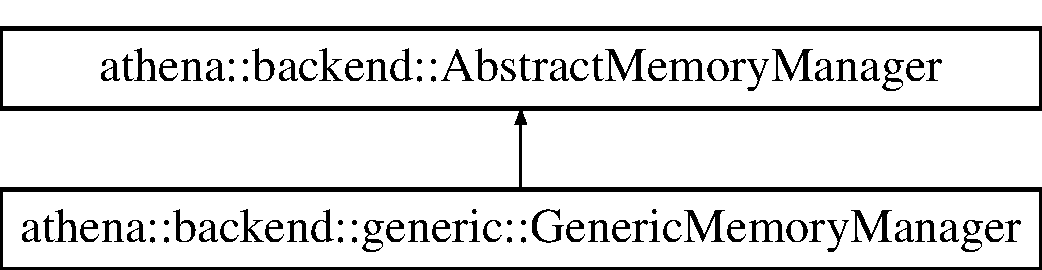
\includegraphics[height=2.000000cm]{d6/d21/classathena_1_1backend_1_1generic_1_1_generic_memory_manager}
\end{center}
\end{figure}
\subsection*{Public Member Functions}
\begin{DoxyCompactItemize}
\item 
void \mbox{\hyperlink{classathena_1_1backend_1_1generic_1_1_generic_memory_manager_a0e39c872b8b41d5239884322988d314d}{init}} () override
\item 
void \mbox{\hyperlink{classathena_1_1backend_1_1generic_1_1_generic_memory_manager_ab90a8874618b851d5309cef66e79d08a}{deinit}} () override
\item 
void $\ast$ \mbox{\hyperlink{classathena_1_1backend_1_1generic_1_1_generic_memory_manager_a7f3dacb56bd95b837910441d0aef1dd8}{get\+Physical\+Address}} (vm\+\_\+word virtual\+Address) override
\item 
void \mbox{\hyperlink{classathena_1_1backend_1_1generic_1_1_generic_memory_manager_aa7fce5a6cbd9c4f5ad1868735e4546a8}{load\+And\+Lock}} (vm\+\_\+word address, unsigned long length) override
\item 
void \mbox{\hyperlink{classathena_1_1backend_1_1generic_1_1_generic_memory_manager_abe837ac5e3bb60c9bc24836788cae679}{allocate\+And\+Lock}} (vm\+\_\+word address, unsigned long length) override
\item 
void \mbox{\hyperlink{classathena_1_1backend_1_1generic_1_1_generic_memory_manager_a58a2b56a07a96c3cabb7b8fd079b3eae}{unlock}} (vm\+\_\+word address) override
\item 
void \mbox{\hyperlink{classathena_1_1backend_1_1generic_1_1_generic_memory_manager_a2767b6c1f5887a2928b665e0c1b454c7}{delete\+From\+Mem}} (vm\+\_\+word address) override
\item 
\mbox{\Hypertarget{classathena_1_1backend_1_1generic_1_1_generic_memory_manager_ad1d29d948806569cce97e9f23ef99ad7}\label{classathena_1_1backend_1_1generic_1_1_generic_memory_manager_ad1d29d948806569cce97e9f23ef99ad7}} 
void {\bfseries set\+Mem\+Size} (size\+\_\+t mem\+Size)
\item 
void \mbox{\hyperlink{classathena_1_1backend_1_1generic_1_1_generic_memory_manager_aa4e2e533d897cf6d042d8a086633bd9d}{set\+Data}} (vm\+\_\+word tensor\+Address, vm\+\_\+word offset, vm\+\_\+word length, void $\ast$data) override
\item 
\mbox{\Hypertarget{classathena_1_1backend_1_1generic_1_1_generic_memory_manager_ad248007976c57e7635ea51d25c7e9f13}\label{classathena_1_1backend_1_1generic_1_1_generic_memory_manager_ad248007976c57e7635ea51d25c7e9f13}} 
void {\bfseries get\+Data} (vm\+\_\+word tensor\+Address, vm\+\_\+word offset, vm\+\_\+word length, void $\ast$data) override
\item 
void \mbox{\hyperlink{classathena_1_1backend_1_1generic_1_1_generic_memory_manager_a2bbfba2a5104aab3068d46214a6ae7df}{load\+And\+Lock}} (\mbox{\hyperlink{classathena_1_1core_1_1_tensor}{athena\+::core\+::\+Tensor}} $\ast$tensor)
\item 
void \mbox{\hyperlink{classathena_1_1backend_1_1generic_1_1_generic_memory_manager_a47ea5a77f81f91f803f748720c5c19b5}{load\+And\+Lock}} (vm\+\_\+word address)
\item 
virtual void \mbox{\hyperlink{classathena_1_1backend_1_1generic_1_1_generic_memory_manager_a9fe52e4020802d6f526fba06adce8407}{load\+And\+Lock}} (vm\+\_\+word address, unsigned long length)=0
\item 
void \mbox{\hyperlink{classathena_1_1backend_1_1generic_1_1_generic_memory_manager_ad40a653a8b32410956ba835ca1bb3e5f}{allocate\+And\+Lock}} (\mbox{\hyperlink{classathena_1_1core_1_1_tensor}{athena\+::core\+::\+Tensor}} $\ast$tensor)
\item 
void \mbox{\hyperlink{classathena_1_1backend_1_1generic_1_1_generic_memory_manager_ab5305b3d1ab91960bf179ce0be166120}{allocate\+And\+Lock}} (vm\+\_\+word address)
\item 
virtual void \mbox{\hyperlink{classathena_1_1backend_1_1generic_1_1_generic_memory_manager_a1b80008e94c21d5ac87f9a45d3f212a8}{allocate\+And\+Lock}} (vm\+\_\+word address, unsigned long length)=0
\end{DoxyCompactItemize}
\subsection*{Protected Member Functions}
\begin{DoxyCompactItemize}
\item 
void \mbox{\hyperlink{classathena_1_1backend_1_1generic_1_1_generic_memory_manager_a46819ceb6e2e55c8c63be980907c3345}{allocation\+Thread\+Func}} (int lane\+Id)
\item 
void \mbox{\hyperlink{classathena_1_1backend_1_1generic_1_1_generic_memory_manager_aec52237e056afc9547aaa89997bdc401}{process\+Queue\+Item}} (\mbox{\hyperlink{structathena_1_1backend_1_1generic_1_1_queue_item}{Queue\+Item}} $\ast$item)
\end{DoxyCompactItemize}
\subsection*{Protected Attributes}
\begin{DoxyCompactItemize}
\item 
\mbox{\Hypertarget{classathena_1_1backend_1_1generic_1_1_generic_memory_manager_ad368d5195616a86b69f9f0d052c2aa34}\label{classathena_1_1backend_1_1generic_1_1_generic_memory_manager_ad368d5195616a86b69f9f0d052c2aa34}} 
std\+::list$<$ \mbox{\hyperlink{structathena_1_1backend_1_1generic_1_1_swap_record}{Swap\+Record}} $\ast$$>$ {\bfseries swap\+Records}
\item 
\mbox{\Hypertarget{classathena_1_1backend_1_1generic_1_1_generic_memory_manager_a99f2c7ed16c2eb288cbcd700d09847ae}\label{classathena_1_1backend_1_1generic_1_1_generic_memory_manager_a99f2c7ed16c2eb288cbcd700d09847ae}} 
\mbox{\hyperlink{structathena_1_1backend_1_1generic_1_1_memory_chunk}{Memory\+Chunk}} $\ast$ {\bfseries memory\+Chunks\+Head}
\item 
\mbox{\Hypertarget{classathena_1_1backend_1_1generic_1_1_generic_memory_manager_a74a52b5bebdd94425f0b8e925a1aca5a}\label{classathena_1_1backend_1_1generic_1_1_generic_memory_manager_a74a52b5bebdd94425f0b8e925a1aca5a}} 
void $\ast$ {\bfseries memory}
\item 
\mbox{\Hypertarget{classathena_1_1backend_1_1generic_1_1_generic_memory_manager_a9b4181cd7b7ad36761b1c3ac72fff3e8}\label{classathena_1_1backend_1_1generic_1_1_generic_memory_manager_a9b4181cd7b7ad36761b1c3ac72fff3e8}} 
std\+::mutex {\bfseries memory\+Chunks\+Lock}
\item 
\mbox{\Hypertarget{classathena_1_1backend_1_1generic_1_1_generic_memory_manager_afcc98bae9917d81728a6f228c41ff623}\label{classathena_1_1backend_1_1generic_1_1_generic_memory_manager_afcc98bae9917d81728a6f228c41ff623}} 
std\+::vector$<$ std\+::thread $>$ {\bfseries mem\+Lanes}
\item 
\mbox{\Hypertarget{classathena_1_1backend_1_1generic_1_1_generic_memory_manager_aaa877b3145831b8476d2f9e575326295}\label{classathena_1_1backend_1_1generic_1_1_generic_memory_manager_aaa877b3145831b8476d2f9e575326295}} 
size\+\_\+t {\bfseries allocated\+Memory}
\item 
\mbox{\Hypertarget{classathena_1_1backend_1_1generic_1_1_generic_memory_manager_a4abaea640cab05ac885bb766da572f6b}\label{classathena_1_1backend_1_1generic_1_1_generic_memory_manager_a4abaea640cab05ac885bb766da572f6b}} 
std\+::queue$<$ \mbox{\hyperlink{structathena_1_1backend_1_1generic_1_1_queue_item}{Queue\+Item}} $\ast$$>$ {\bfseries load\+Queue}
\item 
\mbox{\Hypertarget{classathena_1_1backend_1_1generic_1_1_generic_memory_manager_ab7487c3a37f3fa5c301d992d9e93e1f8}\label{classathena_1_1backend_1_1generic_1_1_generic_memory_manager_ab7487c3a37f3fa5c301d992d9e93e1f8}} 
std\+::vector$<$ bool $>$ {\bfseries lane\+Finished}
\end{DoxyCompactItemize}


\subsection{Detailed Description}
This class implements \mbox{\hyperlink{classathena_1_1backend_1_1_abstract_memory_manager}{Abstract\+Memory\+Manager}} interface for \mbox{\hyperlink{classathena_1_1backend_1_1generic_1_1_generic_executor}{Generic\+Executor}}. It pre-\/allocates R\+AM and uses persistent memory for swap. There are couple memory lanes -\/ threads, that manage R\+AM. They monitor load\+Queue for new queries and move data from hard drive to R\+AM if needed. 

Definition at line 76 of file Generic\+Memory\+Manager.\+h.



\subsection{Member Function Documentation}
\mbox{\Hypertarget{classathena_1_1backend_1_1generic_1_1_generic_memory_manager_abe837ac5e3bb60c9bc24836788cae679}\label{classathena_1_1backend_1_1generic_1_1_generic_memory_manager_abe837ac5e3bb60c9bc24836788cae679}} 
\index{athena\+::backend\+::generic\+::\+Generic\+Memory\+Manager@{athena\+::backend\+::generic\+::\+Generic\+Memory\+Manager}!allocate\+And\+Lock@{allocate\+And\+Lock}}
\index{allocate\+And\+Lock@{allocate\+And\+Lock}!athena\+::backend\+::generic\+::\+Generic\+Memory\+Manager@{athena\+::backend\+::generic\+::\+Generic\+Memory\+Manager}}
\subsubsection{\texorpdfstring{allocate\+And\+Lock()}{allocateAndLock()}\hspace{0.1cm}{\footnotesize\ttfamily [1/4]}}
{\footnotesize\ttfamily void athena\+::backend\+::generic\+::\+Generic\+Memory\+Manager\+::allocate\+And\+Lock (\begin{DoxyParamCaption}\item[{vm\+\_\+word}]{address,  }\item[{unsigned long}]{length }\end{DoxyParamCaption})\hspace{0.3cm}{\ttfamily [override]}, {\ttfamily [virtual]}}

Allocate space in the fastest memory available without loading any data and lock it (prevent from being offloaded) 
\begin{DoxyParams}{Parameters}
{\em address} & Virtual address of Tensor memory is being allocated for \\
\hline
{\em length} & Length in bytes for the piece of memory that is being allocated \\
\hline
\end{DoxyParams}


Implements \mbox{\hyperlink{classathena_1_1backend_1_1_abstract_memory_manager_a1b80008e94c21d5ac87f9a45d3f212a8}{athena\+::backend\+::\+Abstract\+Memory\+Manager}}.



Definition at line 174 of file Generic\+Memory\+Manager.\+cpp.

\mbox{\Hypertarget{classathena_1_1backend_1_1generic_1_1_generic_memory_manager_ad40a653a8b32410956ba835ca1bb3e5f}\label{classathena_1_1backend_1_1generic_1_1_generic_memory_manager_ad40a653a8b32410956ba835ca1bb3e5f}} 
\index{athena\+::backend\+::generic\+::\+Generic\+Memory\+Manager@{athena\+::backend\+::generic\+::\+Generic\+Memory\+Manager}!allocate\+And\+Lock@{allocate\+And\+Lock}}
\index{allocate\+And\+Lock@{allocate\+And\+Lock}!athena\+::backend\+::generic\+::\+Generic\+Memory\+Manager@{athena\+::backend\+::generic\+::\+Generic\+Memory\+Manager}}
\subsubsection{\texorpdfstring{allocate\+And\+Lock()}{allocateAndLock()}\hspace{0.1cm}{\footnotesize\ttfamily [2/4]}}
{\footnotesize\ttfamily void athena\+::backend\+::\+Abstract\+Memory\+Manager\+::allocate\+And\+Lock}

Allocate space in the fastest memory available without loading any data and lock it (prevent from being offloaded) 
\begin{DoxyParams}{Parameters}
{\em tensor} & Tensor memory is being allocated for \\
\hline
\end{DoxyParams}


Definition at line 54 of file Abstract\+Memory\+Manager.\+cpp.

\mbox{\Hypertarget{classathena_1_1backend_1_1generic_1_1_generic_memory_manager_ab5305b3d1ab91960bf179ce0be166120}\label{classathena_1_1backend_1_1generic_1_1_generic_memory_manager_ab5305b3d1ab91960bf179ce0be166120}} 
\index{athena\+::backend\+::generic\+::\+Generic\+Memory\+Manager@{athena\+::backend\+::generic\+::\+Generic\+Memory\+Manager}!allocate\+And\+Lock@{allocate\+And\+Lock}}
\index{allocate\+And\+Lock@{allocate\+And\+Lock}!athena\+::backend\+::generic\+::\+Generic\+Memory\+Manager@{athena\+::backend\+::generic\+::\+Generic\+Memory\+Manager}}
\subsubsection{\texorpdfstring{allocate\+And\+Lock()}{allocateAndLock()}\hspace{0.1cm}{\footnotesize\ttfamily [3/4]}}
{\footnotesize\ttfamily void athena\+::backend\+::\+Abstract\+Memory\+Manager\+::allocate\+And\+Lock}

Allocate space in the fastest memory available without loading any data and lock it (prevent from being offloaded) 
\begin{DoxyParams}{Parameters}
{\em address} & Virtual address of Tensor memory is being allocated for \\
\hline
\end{DoxyParams}


Definition at line 60 of file Abstract\+Memory\+Manager.\+cpp.

\mbox{\Hypertarget{classathena_1_1backend_1_1generic_1_1_generic_memory_manager_a1b80008e94c21d5ac87f9a45d3f212a8}\label{classathena_1_1backend_1_1generic_1_1_generic_memory_manager_a1b80008e94c21d5ac87f9a45d3f212a8}} 
\index{athena\+::backend\+::generic\+::\+Generic\+Memory\+Manager@{athena\+::backend\+::generic\+::\+Generic\+Memory\+Manager}!allocate\+And\+Lock@{allocate\+And\+Lock}}
\index{allocate\+And\+Lock@{allocate\+And\+Lock}!athena\+::backend\+::generic\+::\+Generic\+Memory\+Manager@{athena\+::backend\+::generic\+::\+Generic\+Memory\+Manager}}
\subsubsection{\texorpdfstring{allocate\+And\+Lock()}{allocateAndLock()}\hspace{0.1cm}{\footnotesize\ttfamily [4/4]}}
{\footnotesize\ttfamily virtual void athena\+::backend\+::\+Abstract\+Memory\+Manager\+::allocate\+And\+Lock}

Allocate space in the fastest memory available without loading any data and lock it (prevent from being offloaded) 
\begin{DoxyParams}{Parameters}
{\em address} & Virtual address of Tensor memory is being allocated for \\
\hline
{\em length} & Length in bytes for the piece of memory that is being allocated \\
\hline
\end{DoxyParams}
\mbox{\Hypertarget{classathena_1_1backend_1_1generic_1_1_generic_memory_manager_a46819ceb6e2e55c8c63be980907c3345}\label{classathena_1_1backend_1_1generic_1_1_generic_memory_manager_a46819ceb6e2e55c8c63be980907c3345}} 
\index{athena\+::backend\+::generic\+::\+Generic\+Memory\+Manager@{athena\+::backend\+::generic\+::\+Generic\+Memory\+Manager}!allocation\+Thread\+Func@{allocation\+Thread\+Func}}
\index{allocation\+Thread\+Func@{allocation\+Thread\+Func}!athena\+::backend\+::generic\+::\+Generic\+Memory\+Manager@{athena\+::backend\+::generic\+::\+Generic\+Memory\+Manager}}
\subsubsection{\texorpdfstring{allocation\+Thread\+Func()}{allocationThreadFunc()}}
{\footnotesize\ttfamily void athena\+::backend\+::generic\+::\+Generic\+Memory\+Manager\+::allocation\+Thread\+Func (\begin{DoxyParamCaption}\item[{int}]{lane\+Id }\end{DoxyParamCaption})\hspace{0.3cm}{\ttfamily [protected]}}

This is a thread function for memory lane-\/threads. It loads data to R\+AM and notifies corresponding threads 
\begin{DoxyParams}{Parameters}
{\em lane\+Id} & \\
\hline
\end{DoxyParams}


Definition at line 37 of file Generic\+Memory\+Manager.\+cpp.



Referenced by init().

\mbox{\Hypertarget{classathena_1_1backend_1_1generic_1_1_generic_memory_manager_ab90a8874618b851d5309cef66e79d08a}\label{classathena_1_1backend_1_1generic_1_1_generic_memory_manager_ab90a8874618b851d5309cef66e79d08a}} 
\index{athena\+::backend\+::generic\+::\+Generic\+Memory\+Manager@{athena\+::backend\+::generic\+::\+Generic\+Memory\+Manager}!deinit@{deinit}}
\index{deinit@{deinit}!athena\+::backend\+::generic\+::\+Generic\+Memory\+Manager@{athena\+::backend\+::generic\+::\+Generic\+Memory\+Manager}}
\subsubsection{\texorpdfstring{deinit()}{deinit()}}
{\footnotesize\ttfamily void athena\+::backend\+::generic\+::\+Generic\+Memory\+Manager\+::deinit (\begin{DoxyParamCaption}{ }\end{DoxyParamCaption})\hspace{0.3cm}{\ttfamily [override]}, {\ttfamily [virtual]}}

Free R\+AM and stop all threads-\/memory lanes 

Implements \mbox{\hyperlink{classathena_1_1backend_1_1_abstract_memory_manager}{athena\+::backend\+::\+Abstract\+Memory\+Manager}}.



Definition at line 84 of file Generic\+Memory\+Manager.\+cpp.

\mbox{\Hypertarget{classathena_1_1backend_1_1generic_1_1_generic_memory_manager_a2767b6c1f5887a2928b665e0c1b454c7}\label{classathena_1_1backend_1_1generic_1_1_generic_memory_manager_a2767b6c1f5887a2928b665e0c1b454c7}} 
\index{athena\+::backend\+::generic\+::\+Generic\+Memory\+Manager@{athena\+::backend\+::generic\+::\+Generic\+Memory\+Manager}!delete\+From\+Mem@{delete\+From\+Mem}}
\index{delete\+From\+Mem@{delete\+From\+Mem}!athena\+::backend\+::generic\+::\+Generic\+Memory\+Manager@{athena\+::backend\+::generic\+::\+Generic\+Memory\+Manager}}
\subsubsection{\texorpdfstring{delete\+From\+Mem()}{deleteFromMem()}}
{\footnotesize\ttfamily void athena\+::backend\+::generic\+::\+Generic\+Memory\+Manager\+::delete\+From\+Mem (\begin{DoxyParamCaption}\item[{vm\+\_\+word}]{address }\end{DoxyParamCaption})\hspace{0.3cm}{\ttfamily [override]}, {\ttfamily [virtual]}}

Mark corresponding memory chunk as free 
\begin{DoxyParams}{Parameters}
{\em address} & Virtual address \\
\hline
\end{DoxyParams}


Implements \mbox{\hyperlink{classathena_1_1backend_1_1_abstract_memory_manager_a8ffd6cf21559978f394e2e11815506b5}{athena\+::backend\+::\+Abstract\+Memory\+Manager}}.



Definition at line 148 of file Generic\+Memory\+Manager.\+cpp.

\mbox{\Hypertarget{classathena_1_1backend_1_1generic_1_1_generic_memory_manager_a7f3dacb56bd95b837910441d0aef1dd8}\label{classathena_1_1backend_1_1generic_1_1_generic_memory_manager_a7f3dacb56bd95b837910441d0aef1dd8}} 
\index{athena\+::backend\+::generic\+::\+Generic\+Memory\+Manager@{athena\+::backend\+::generic\+::\+Generic\+Memory\+Manager}!get\+Physical\+Address@{get\+Physical\+Address}}
\index{get\+Physical\+Address@{get\+Physical\+Address}!athena\+::backend\+::generic\+::\+Generic\+Memory\+Manager@{athena\+::backend\+::generic\+::\+Generic\+Memory\+Manager}}
\subsubsection{\texorpdfstring{get\+Physical\+Address()}{getPhysicalAddress()}}
{\footnotesize\ttfamily void $\ast$ athena\+::backend\+::generic\+::\+Generic\+Memory\+Manager\+::get\+Physical\+Address (\begin{DoxyParamCaption}\item[{vm\+\_\+word}]{virtual\+Address }\end{DoxyParamCaption})\hspace{0.3cm}{\ttfamily [override]}, {\ttfamily [virtual]}}

Convert virtual address to physical one 
\begin{DoxyParams}{Parameters}
{\em virtual\+Address} & Virtual address, unsigned long from 0 to 2$^\wedge$64-\/1 \\
\hline
\end{DoxyParams}
\begin{DoxyReturn}{Returns}
Pointer to physical memory 
\end{DoxyReturn}


Implements \mbox{\hyperlink{classathena_1_1backend_1_1_abstract_memory_manager_ad441d7a2281f5f2b2627272d136f72b8}{athena\+::backend\+::\+Abstract\+Memory\+Manager}}.



Definition at line 51 of file Generic\+Memory\+Manager.\+cpp.

\mbox{\Hypertarget{classathena_1_1backend_1_1generic_1_1_generic_memory_manager_a0e39c872b8b41d5239884322988d314d}\label{classathena_1_1backend_1_1generic_1_1_generic_memory_manager_a0e39c872b8b41d5239884322988d314d}} 
\index{athena\+::backend\+::generic\+::\+Generic\+Memory\+Manager@{athena\+::backend\+::generic\+::\+Generic\+Memory\+Manager}!init@{init}}
\index{init@{init}!athena\+::backend\+::generic\+::\+Generic\+Memory\+Manager@{athena\+::backend\+::generic\+::\+Generic\+Memory\+Manager}}
\subsubsection{\texorpdfstring{init()}{init()}}
{\footnotesize\ttfamily void athena\+::backend\+::generic\+::\+Generic\+Memory\+Manager\+::init (\begin{DoxyParamCaption}{ }\end{DoxyParamCaption})\hspace{0.3cm}{\ttfamily [override]}, {\ttfamily [virtual]}}

Initialize memory manager. That\textquotesingle{}s where actual memory allocation happens. All configurations should be done before this method is called. 

Implements \mbox{\hyperlink{classathena_1_1backend_1_1_abstract_memory_manager}{athena\+::backend\+::\+Abstract\+Memory\+Manager}}.



Definition at line 18 of file Generic\+Memory\+Manager.\+cpp.

\mbox{\Hypertarget{classathena_1_1backend_1_1generic_1_1_generic_memory_manager_aa7fce5a6cbd9c4f5ad1868735e4546a8}\label{classathena_1_1backend_1_1generic_1_1_generic_memory_manager_aa7fce5a6cbd9c4f5ad1868735e4546a8}} 
\index{athena\+::backend\+::generic\+::\+Generic\+Memory\+Manager@{athena\+::backend\+::generic\+::\+Generic\+Memory\+Manager}!load\+And\+Lock@{load\+And\+Lock}}
\index{load\+And\+Lock@{load\+And\+Lock}!athena\+::backend\+::generic\+::\+Generic\+Memory\+Manager@{athena\+::backend\+::generic\+::\+Generic\+Memory\+Manager}}
\subsubsection{\texorpdfstring{load\+And\+Lock()}{loadAndLock()}\hspace{0.1cm}{\footnotesize\ttfamily [1/4]}}
{\footnotesize\ttfamily void athena\+::backend\+::generic\+::\+Generic\+Memory\+Manager\+::load\+And\+Lock (\begin{DoxyParamCaption}\item[{vm\+\_\+word}]{address,  }\item[{unsigned long}]{length }\end{DoxyParamCaption})\hspace{0.3cm}{\ttfamily [override]}, {\ttfamily [virtual]}}

Move data to the fastest memory type available (e.\+g. from hard drive to R\+AM) and lock it (prevent from being offloaded) 
\begin{DoxyParams}{Parameters}
{\em address} & Virtual address \\
\hline
{\em length} & Size of Tensor in bytes \\
\hline
\end{DoxyParams}


Implements \mbox{\hyperlink{classathena_1_1backend_1_1_abstract_memory_manager_a9fe52e4020802d6f526fba06adce8407}{athena\+::backend\+::\+Abstract\+Memory\+Manager}}.



Definition at line 65 of file Generic\+Memory\+Manager.\+cpp.

\mbox{\Hypertarget{classathena_1_1backend_1_1generic_1_1_generic_memory_manager_a47ea5a77f81f91f803f748720c5c19b5}\label{classathena_1_1backend_1_1generic_1_1_generic_memory_manager_a47ea5a77f81f91f803f748720c5c19b5}} 
\index{athena\+::backend\+::generic\+::\+Generic\+Memory\+Manager@{athena\+::backend\+::generic\+::\+Generic\+Memory\+Manager}!load\+And\+Lock@{load\+And\+Lock}}
\index{load\+And\+Lock@{load\+And\+Lock}!athena\+::backend\+::generic\+::\+Generic\+Memory\+Manager@{athena\+::backend\+::generic\+::\+Generic\+Memory\+Manager}}
\subsubsection{\texorpdfstring{load\+And\+Lock()}{loadAndLock()}\hspace{0.1cm}{\footnotesize\ttfamily [2/4]}}
{\footnotesize\ttfamily void athena\+::backend\+::\+Abstract\+Memory\+Manager\+::load\+And\+Lock}

Move data to the fastest memory type available (e.\+g. from hard drive to R\+AM) and lock it (prevent from being offloaded) 
\begin{DoxyParams}{Parameters}
{\em address} & Virtual address of Tensor containing data \\
\hline
\end{DoxyParams}


Definition at line 30 of file Abstract\+Memory\+Manager.\+cpp.

\mbox{\Hypertarget{classathena_1_1backend_1_1generic_1_1_generic_memory_manager_a2bbfba2a5104aab3068d46214a6ae7df}\label{classathena_1_1backend_1_1generic_1_1_generic_memory_manager_a2bbfba2a5104aab3068d46214a6ae7df}} 
\index{athena\+::backend\+::generic\+::\+Generic\+Memory\+Manager@{athena\+::backend\+::generic\+::\+Generic\+Memory\+Manager}!load\+And\+Lock@{load\+And\+Lock}}
\index{load\+And\+Lock@{load\+And\+Lock}!athena\+::backend\+::generic\+::\+Generic\+Memory\+Manager@{athena\+::backend\+::generic\+::\+Generic\+Memory\+Manager}}
\subsubsection{\texorpdfstring{load\+And\+Lock()}{loadAndLock()}\hspace{0.1cm}{\footnotesize\ttfamily [3/4]}}
{\footnotesize\ttfamily void athena\+::backend\+::\+Abstract\+Memory\+Manager\+::load\+And\+Lock}

Move data to the fastest memory type available (e.\+g. from hard drive to R\+AM) and lock it (prevent from being offloaded) 
\begin{DoxyParams}{Parameters}
{\em tensor} & Tensor containing data \\
\hline
\end{DoxyParams}


Definition at line 25 of file Abstract\+Memory\+Manager.\+cpp.

\mbox{\Hypertarget{classathena_1_1backend_1_1generic_1_1_generic_memory_manager_a9fe52e4020802d6f526fba06adce8407}\label{classathena_1_1backend_1_1generic_1_1_generic_memory_manager_a9fe52e4020802d6f526fba06adce8407}} 
\index{athena\+::backend\+::generic\+::\+Generic\+Memory\+Manager@{athena\+::backend\+::generic\+::\+Generic\+Memory\+Manager}!load\+And\+Lock@{load\+And\+Lock}}
\index{load\+And\+Lock@{load\+And\+Lock}!athena\+::backend\+::generic\+::\+Generic\+Memory\+Manager@{athena\+::backend\+::generic\+::\+Generic\+Memory\+Manager}}
\subsubsection{\texorpdfstring{load\+And\+Lock()}{loadAndLock()}\hspace{0.1cm}{\footnotesize\ttfamily [4/4]}}
{\footnotesize\ttfamily virtual void athena\+::backend\+::\+Abstract\+Memory\+Manager\+::load\+And\+Lock}

Move data to the fastest memory type available (e.\+g. from hard drive to R\+AM) and lock it (prevent from being offloaded) 
\begin{DoxyParams}{Parameters}
{\em address} & Virtual address \\
\hline
{\em length} & Size of Tensor in bytes \\
\hline
\end{DoxyParams}
\mbox{\Hypertarget{classathena_1_1backend_1_1generic_1_1_generic_memory_manager_aec52237e056afc9547aaa89997bdc401}\label{classathena_1_1backend_1_1generic_1_1_generic_memory_manager_aec52237e056afc9547aaa89997bdc401}} 
\index{athena\+::backend\+::generic\+::\+Generic\+Memory\+Manager@{athena\+::backend\+::generic\+::\+Generic\+Memory\+Manager}!process\+Queue\+Item@{process\+Queue\+Item}}
\index{process\+Queue\+Item@{process\+Queue\+Item}!athena\+::backend\+::generic\+::\+Generic\+Memory\+Manager@{athena\+::backend\+::generic\+::\+Generic\+Memory\+Manager}}
\subsubsection{\texorpdfstring{process\+Queue\+Item()}{processQueueItem()}}
{\footnotesize\ttfamily void athena\+::backend\+::generic\+::\+Generic\+Memory\+Manager\+::process\+Queue\+Item (\begin{DoxyParamCaption}\item[{\mbox{\hyperlink{structathena_1_1backend_1_1generic_1_1_queue_item}{Queue\+Item}} $\ast$}]{item }\end{DoxyParamCaption})\hspace{0.3cm}{\ttfamily [protected]}}

This method does actual physical memory allocation 
\begin{DoxyParams}{Parameters}
{\em item} & \\
\hline
\end{DoxyParams}


Definition at line 219 of file Generic\+Memory\+Manager.\+cpp.

\mbox{\Hypertarget{classathena_1_1backend_1_1generic_1_1_generic_memory_manager_aa4e2e533d897cf6d042d8a086633bd9d}\label{classathena_1_1backend_1_1generic_1_1_generic_memory_manager_aa4e2e533d897cf6d042d8a086633bd9d}} 
\index{athena\+::backend\+::generic\+::\+Generic\+Memory\+Manager@{athena\+::backend\+::generic\+::\+Generic\+Memory\+Manager}!set\+Data@{set\+Data}}
\index{set\+Data@{set\+Data}!athena\+::backend\+::generic\+::\+Generic\+Memory\+Manager@{athena\+::backend\+::generic\+::\+Generic\+Memory\+Manager}}
\subsubsection{\texorpdfstring{set\+Data()}{setData()}}
{\footnotesize\ttfamily void athena\+::backend\+::generic\+::\+Generic\+Memory\+Manager\+::set\+Data (\begin{DoxyParamCaption}\item[{vm\+\_\+word}]{tensor\+Address,  }\item[{vm\+\_\+word}]{offset,  }\item[{vm\+\_\+word}]{length,  }\item[{void $\ast$}]{data }\end{DoxyParamCaption})\hspace{0.3cm}{\ttfamily [override]}, {\ttfamily [virtual]}}

Sets memory with the data 
\begin{DoxyParams}{Parameters}
{\em tensor\+Address} & Virtual address of Tensor beginning (see Tensor\+::get\+Start\+Address) \\
\hline
{\em offset} & Offset in bytes from the beginning \\
\hline
{\em length} & Length of piece of data in bytes \\
\hline
{\em data} & Pointer to data \\
\hline
\end{DoxyParams}


Implements \mbox{\hyperlink{classathena_1_1backend_1_1_abstract_memory_manager_a18562c6f336ff0f7ff800f877696c851}{athena\+::backend\+::\+Abstract\+Memory\+Manager}}.



Definition at line 195 of file Generic\+Memory\+Manager.\+cpp.

\mbox{\Hypertarget{classathena_1_1backend_1_1generic_1_1_generic_memory_manager_a58a2b56a07a96c3cabb7b8fd079b3eae}\label{classathena_1_1backend_1_1generic_1_1_generic_memory_manager_a58a2b56a07a96c3cabb7b8fd079b3eae}} 
\index{athena\+::backend\+::generic\+::\+Generic\+Memory\+Manager@{athena\+::backend\+::generic\+::\+Generic\+Memory\+Manager}!unlock@{unlock}}
\index{unlock@{unlock}!athena\+::backend\+::generic\+::\+Generic\+Memory\+Manager@{athena\+::backend\+::generic\+::\+Generic\+Memory\+Manager}}
\subsubsection{\texorpdfstring{unlock()}{unlock()}}
{\footnotesize\ttfamily void athena\+::backend\+::generic\+::\+Generic\+Memory\+Manager\+::unlock (\begin{DoxyParamCaption}\item[{vm\+\_\+word}]{address }\end{DoxyParamCaption})\hspace{0.3cm}{\ttfamily [override]}, {\ttfamily [virtual]}}

Lets data be offloaded to a slower memory type (e.\+g. from R\+AM to H\+DD) 
\begin{DoxyParams}{Parameters}
{\em address} & Virtual address \\
\hline
\end{DoxyParams}


Implements \mbox{\hyperlink{classathena_1_1backend_1_1_abstract_memory_manager_aec859ee3bf6011d8710b2ec4bfc2373e}{athena\+::backend\+::\+Abstract\+Memory\+Manager}}.



Definition at line 105 of file Generic\+Memory\+Manager.\+cpp.



The documentation for this class was generated from the following files\+:\begin{DoxyCompactItemize}
\item 
backend/generic/Generic\+Memory\+Manager.\+h\item 
backend/generic/Generic\+Memory\+Manager.\+cpp\end{DoxyCompactItemize}

\hypertarget{classathena_1_1core_1_1optimizers_1_1_gradient_descent}{}\section{athena\+:\+:core\+:\+:optimizers\+:\+:Gradient\+Descent Class Reference}
\label{classathena_1_1core_1_1optimizers_1_1_gradient_descent}\index{athena\+::core\+::optimizers\+::\+Gradient\+Descent@{athena\+::core\+::optimizers\+::\+Gradient\+Descent}}
Inheritance diagram for athena\+:\+:core\+:\+:optimizers\+:\+:Gradient\+Descent\+:\begin{figure}[H]
\begin{center}
\leavevmode
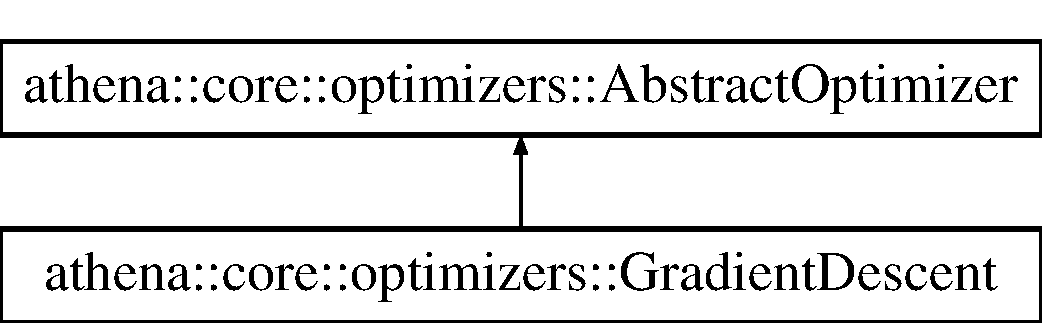
\includegraphics[height=2.000000cm]{dd/d53/classathena_1_1core_1_1optimizers_1_1_gradient_descent}
\end{center}
\end{figure}
\subsection*{Public Member Functions}
\begin{DoxyCompactItemize}
\item 
\mbox{\Hypertarget{classathena_1_1core_1_1optimizers_1_1_gradient_descent_a1f81ba3b4a6291f37a33f7eb903ecdfe}\label{classathena_1_1core_1_1optimizers_1_1_gradient_descent_a1f81ba3b4a6291f37a33f7eb903ecdfe}} 
{\bfseries Gradient\+Descent} (\mbox{\hyperlink{classathena_1_1core_1_1loss_1_1_abstract_loss_function}{athena\+::core\+::loss\+::\+Abstract\+Loss\+Function}} $\ast$loss, float learning\+Rate)
\item 
\mbox{\Hypertarget{classathena_1_1core_1_1optimizers_1_1_gradient_descent_ab9ecd3b02a82c86bfaaa3d93789d2d5a}\label{classathena_1_1core_1_1optimizers_1_1_gradient_descent_ab9ecd3b02a82c86bfaaa3d93789d2d5a}} 
void {\bfseries prepare} () override
\item 
\mbox{\Hypertarget{classathena_1_1core_1_1optimizers_1_1_gradient_descent_a1403aaa8543b4f50e783ae19b26e2ea4}\label{classathena_1_1core_1_1optimizers_1_1_gradient_descent_a1403aaa8543b4f50e783ae19b26e2ea4}} 
void {\bfseries minimize} () override
\end{DoxyCompactItemize}
\subsection*{Protected Member Functions}
\begin{DoxyCompactItemize}
\item 
\mbox{\Hypertarget{classathena_1_1core_1_1optimizers_1_1_gradient_descent_afadd2e418a6ed2a2b025b5cffdfa7d4c}\label{classathena_1_1core_1_1optimizers_1_1_gradient_descent_afadd2e418a6ed2a2b025b5cffdfa7d4c}} 
std\+::tuple$<$ std\+::vector$<$ unsigned long $>$, unsigned long $>$ {\bfseries get\+Byte\+Code} (\mbox{\hyperlink{classathena_1_1core_1_1loss_1_1_abstract_loss_function}{athena\+::core\+::loss\+::\+Abstract\+Loss\+Function}} $\ast$node)
\end{DoxyCompactItemize}
\subsection*{Protected Attributes}
\begin{DoxyCompactItemize}
\item 
\mbox{\Hypertarget{classathena_1_1core_1_1optimizers_1_1_gradient_descent_a40fd65d38f6804e2e8c7109f7cd27e67}\label{classathena_1_1core_1_1optimizers_1_1_gradient_descent_a40fd65d38f6804e2e8c7109f7cd27e67}} 
float {\bfseries learning\+Rate}
\end{DoxyCompactItemize}


\subsection{Detailed Description}


Definition at line 12 of file Gradient\+Descent.\+h.



The documentation for this class was generated from the following files\+:\begin{DoxyCompactItemize}
\item 
core/optimizers/Gradient\+Descent.\+h\item 
core/optimizers/Gradient\+Descent.\+cpp\end{DoxyCompactItemize}

\hypertarget{classathena_1_1core_1_1_input_node}{}\section{athena\+:\+:core\+:\+:Input\+Node Class Reference}
\label{classathena_1_1core_1_1_input_node}\index{athena\+::core\+::\+Input\+Node@{athena\+::core\+::\+Input\+Node}}


{\ttfamily \#include $<$Input\+Node.\+h$>$}

Inheritance diagram for athena\+:\+:core\+:\+:Input\+Node\+:\begin{figure}[H]
\begin{center}
\leavevmode
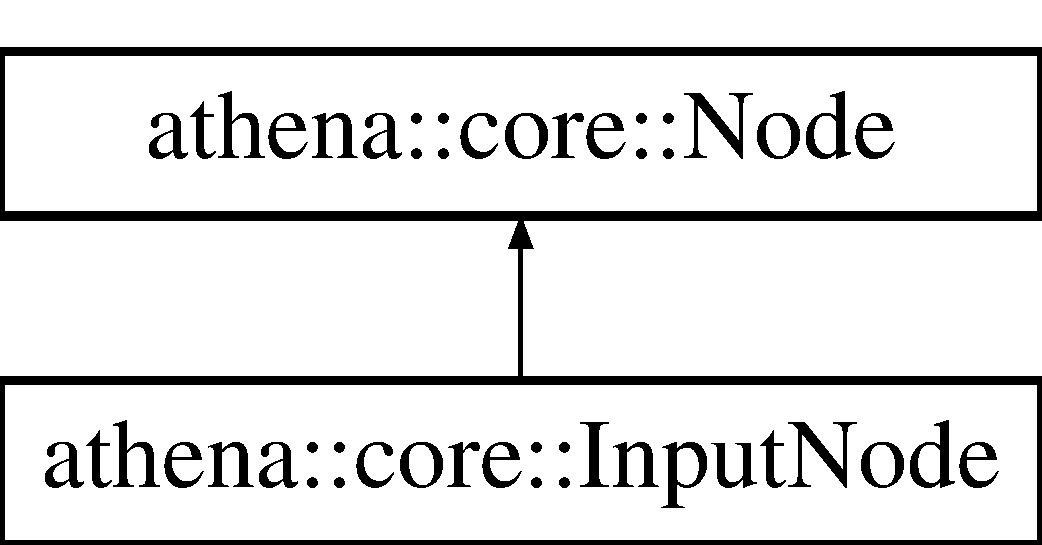
\includegraphics[height=2.000000cm]{classathena_1_1core_1_1_input_node}
\end{center}
\end{figure}
\subsection*{Public Member Functions}
\begin{DoxyCompactItemize}
\item 
\mbox{\Hypertarget{classathena_1_1core_1_1_input_node_a14987336678cfcbc2ddbd3f6b67bb572}\label{classathena_1_1core_1_1_input_node_a14987336678cfcbc2ddbd3f6b67bb572}} 
{\bfseries Input\+Node} (\mbox{\hyperlink{classathena_1_1core_1_1_tensor}{Tensor}} $\ast$input, bool \mbox{\hyperlink{classathena_1_1core_1_1_input_node_a4be7482bcf2e56ea3fd03a2bf79be074}{is\+Frozen}}=true)
\item 
bool \mbox{\hyperlink{classathena_1_1core_1_1_input_node_a2548b569a336b75c0005295833052979}{is\+Input\+Node}} () override
\item 
void \mbox{\hyperlink{classathena_1_1core_1_1_input_node_a8c17ce96d989454e6316c1c049c2c98d}{set\+Mapped\+Mem\+Cell}} (unsigned long cell)
\item 
unsigned long \mbox{\hyperlink{classathena_1_1core_1_1_input_node_acebc0cbf077eaae99f5c11cfba608533}{get\+Mapped\+Mem\+Cell}} ()
\item 
void \mbox{\hyperlink{classathena_1_1core_1_1_input_node_aaec12f4c76b6d9890efe1fb4337a1b61}{after}} (\mbox{\hyperlink{classathena_1_1core_1_1_node}{Node}} $\ast$) override
\item 
\mbox{\hyperlink{classathena_1_1core_1_1_tensor}{Tensor}} $\ast$ \mbox{\hyperlink{classathena_1_1core_1_1_input_node_a983588a56beeb817a59cf9b7e4a63b55}{get\+Data}} ()
\item 
bool \mbox{\hyperlink{classathena_1_1core_1_1_input_node_a4be7482bcf2e56ea3fd03a2bf79be074}{is\+Frozen}} ()
\item 
void \mbox{\hyperlink{classathena_1_1core_1_1_input_node_a45311e1bbff5dd28df3c3877aaa10109}{set\+Frozen}} (bool frozen)
\item 
\mbox{\Hypertarget{classathena_1_1core_1_1_input_node_a165dadd24956ef927c4342e9d365c46d}\label{classathena_1_1core_1_1_input_node_a165dadd24956ef927c4342e9d365c46d}} 
void {\bfseries set\+Initializer} (\mbox{\hyperlink{classathena_1_1core_1_1initializers_1_1_abstract_initializer}{athena\+::core\+::initializers\+::\+Abstract\+Initializer}} $\ast$initializer)
\item 
\mbox{\Hypertarget{classathena_1_1core_1_1_input_node_a1032db02e6706b02b8bb72d68709402b}\label{classathena_1_1core_1_1_input_node_a1032db02e6706b02b8bb72d68709402b}} 
\mbox{\hyperlink{classathena_1_1core_1_1initializers_1_1_abstract_initializer}{athena\+::core\+::initializers\+::\+Abstract\+Initializer}} $\ast$ {\bfseries get\+Initializer} ()
\end{DoxyCompactItemize}
\subsection*{Additional Inherited Members}


\subsection{Detailed Description}
Subclass of \mbox{\hyperlink{classathena_1_1core_1_1_node}{athena\+::core\+::\+Node}} Represents a node that has no predecessors 

\subsection{Member Function Documentation}
\mbox{\Hypertarget{classathena_1_1core_1_1_input_node_aaec12f4c76b6d9890efe1fb4337a1b61}\label{classathena_1_1core_1_1_input_node_aaec12f4c76b6d9890efe1fb4337a1b61}} 
\index{athena\+::core\+::\+Input\+Node@{athena\+::core\+::\+Input\+Node}!after@{after}}
\index{after@{after}!athena\+::core\+::\+Input\+Node@{athena\+::core\+::\+Input\+Node}}
\subsubsection{\texorpdfstring{after()}{after()}}
{\footnotesize\ttfamily void athena\+::core\+::\+Input\+Node\+::after (\begin{DoxyParamCaption}\item[{\mbox{\hyperlink{classathena_1_1core_1_1_node}{Node}} $\ast$}]{ }\end{DoxyParamCaption})\hspace{0.3cm}{\ttfamily [inline]}, {\ttfamily [override]}, {\ttfamily [virtual]}}

Input\+Nodes can\textquotesingle{}t be placed after other nodes in Athena\textquotesingle{}s execution graph. This method does nothing 

Reimplemented from \mbox{\hyperlink{classathena_1_1core_1_1_node_aefef588463c8e215e998415a7cc6b320}{athena\+::core\+::\+Node}}.

\mbox{\Hypertarget{classathena_1_1core_1_1_input_node_a983588a56beeb817a59cf9b7e4a63b55}\label{classathena_1_1core_1_1_input_node_a983588a56beeb817a59cf9b7e4a63b55}} 
\index{athena\+::core\+::\+Input\+Node@{athena\+::core\+::\+Input\+Node}!get\+Data@{get\+Data}}
\index{get\+Data@{get\+Data}!athena\+::core\+::\+Input\+Node@{athena\+::core\+::\+Input\+Node}}
\subsubsection{\texorpdfstring{get\+Data()}{getData()}}
{\footnotesize\ttfamily \mbox{\hyperlink{classathena_1_1core_1_1_tensor}{athena\+::core\+::\+Tensor}} $\ast$ athena\+::core\+::\+Input\+Node\+::get\+Data (\begin{DoxyParamCaption}{ }\end{DoxyParamCaption})}

Get data associated with this \mbox{\hyperlink{classathena_1_1core_1_1_input_node}{Input\+Node}} \begin{DoxyReturn}{Returns}
Pointer to \mbox{\hyperlink{classathena_1_1core_1_1_tensor}{Tensor}} 
\end{DoxyReturn}
\mbox{\Hypertarget{classathena_1_1core_1_1_input_node_acebc0cbf077eaae99f5c11cfba608533}\label{classathena_1_1core_1_1_input_node_acebc0cbf077eaae99f5c11cfba608533}} 
\index{athena\+::core\+::\+Input\+Node@{athena\+::core\+::\+Input\+Node}!get\+Mapped\+Mem\+Cell@{get\+Mapped\+Mem\+Cell}}
\index{get\+Mapped\+Mem\+Cell@{get\+Mapped\+Mem\+Cell}!athena\+::core\+::\+Input\+Node@{athena\+::core\+::\+Input\+Node}}
\subsubsection{\texorpdfstring{get\+Mapped\+Mem\+Cell()}{getMappedMemCell()}}
{\footnotesize\ttfamily unsigned long athena\+::core\+::\+Input\+Node\+::get\+Mapped\+Mem\+Cell (\begin{DoxyParamCaption}{ }\end{DoxyParamCaption})}

Get the number of memory cell that is used to store tensor for this node \begin{DoxyReturn}{Returns}
Memory cell number 
\end{DoxyReturn}
\mbox{\Hypertarget{classathena_1_1core_1_1_input_node_a4be7482bcf2e56ea3fd03a2bf79be074}\label{classathena_1_1core_1_1_input_node_a4be7482bcf2e56ea3fd03a2bf79be074}} 
\index{athena\+::core\+::\+Input\+Node@{athena\+::core\+::\+Input\+Node}!is\+Frozen@{is\+Frozen}}
\index{is\+Frozen@{is\+Frozen}!athena\+::core\+::\+Input\+Node@{athena\+::core\+::\+Input\+Node}}
\subsubsection{\texorpdfstring{is\+Frozen()}{isFrozen()}}
{\footnotesize\ttfamily bool athena\+::core\+::\+Input\+Node\+::is\+Frozen (\begin{DoxyParamCaption}{ }\end{DoxyParamCaption})}

Input\+Nodes can be frozen. This means their tensors won\textquotesingle{}t be changed during back propagation process (e.\+g. \mbox{\hyperlink{classathena_1_1core_1_1_input_node}{Input\+Node}} contains your input data). By default new Input\+Nodes are frozen. \begin{DoxyReturn}{Returns}
Current freeze state 
\end{DoxyReturn}
\mbox{\Hypertarget{classathena_1_1core_1_1_input_node_a2548b569a336b75c0005295833052979}\label{classathena_1_1core_1_1_input_node_a2548b569a336b75c0005295833052979}} 
\index{athena\+::core\+::\+Input\+Node@{athena\+::core\+::\+Input\+Node}!is\+Input\+Node@{is\+Input\+Node}}
\index{is\+Input\+Node@{is\+Input\+Node}!athena\+::core\+::\+Input\+Node@{athena\+::core\+::\+Input\+Node}}
\subsubsection{\texorpdfstring{is\+Input\+Node()}{isInputNode()}}
{\footnotesize\ttfamily bool athena\+::core\+::\+Input\+Node\+::is\+Input\+Node (\begin{DoxyParamCaption}{ }\end{DoxyParamCaption})\hspace{0.3cm}{\ttfamily [override]}, {\ttfamily [virtual]}}

Check if it is an input node \begin{DoxyReturn}{Returns}
true 
\end{DoxyReturn}


Reimplemented from \mbox{\hyperlink{classathena_1_1core_1_1_node_a6ae012557fc6b29127366b1e92801d4a}{athena\+::core\+::\+Node}}.

\mbox{\Hypertarget{classathena_1_1core_1_1_input_node_a45311e1bbff5dd28df3c3877aaa10109}\label{classathena_1_1core_1_1_input_node_a45311e1bbff5dd28df3c3877aaa10109}} 
\index{athena\+::core\+::\+Input\+Node@{athena\+::core\+::\+Input\+Node}!set\+Frozen@{set\+Frozen}}
\index{set\+Frozen@{set\+Frozen}!athena\+::core\+::\+Input\+Node@{athena\+::core\+::\+Input\+Node}}
\subsubsection{\texorpdfstring{set\+Frozen()}{setFrozen()}}
{\footnotesize\ttfamily void athena\+::core\+::\+Input\+Node\+::set\+Frozen (\begin{DoxyParamCaption}\item[{bool}]{frozen }\end{DoxyParamCaption})}

Input\+Nodes can be frozen. This means their tensors won\textquotesingle{}t be changed during back propagation process (e.\+g. \mbox{\hyperlink{classathena_1_1core_1_1_input_node}{Input\+Node}} contains your input data). By default new Input\+Nodes are frozen. 
\begin{DoxyParams}{Parameters}
{\em frozen} & True -\/ freeze node, False -\/ unfreeze node (make it variable) \\
\hline
\end{DoxyParams}
\mbox{\Hypertarget{classathena_1_1core_1_1_input_node_a8c17ce96d989454e6316c1c049c2c98d}\label{classathena_1_1core_1_1_input_node_a8c17ce96d989454e6316c1c049c2c98d}} 
\index{athena\+::core\+::\+Input\+Node@{athena\+::core\+::\+Input\+Node}!set\+Mapped\+Mem\+Cell@{set\+Mapped\+Mem\+Cell}}
\index{set\+Mapped\+Mem\+Cell@{set\+Mapped\+Mem\+Cell}!athena\+::core\+::\+Input\+Node@{athena\+::core\+::\+Input\+Node}}
\subsubsection{\texorpdfstring{set\+Mapped\+Mem\+Cell()}{setMappedMemCell()}}
{\footnotesize\ttfamily void athena\+::core\+::\+Input\+Node\+::set\+Mapped\+Mem\+Cell (\begin{DoxyParamCaption}\item[{unsigned long}]{cell }\end{DoxyParamCaption})}

Specify which memory cell will be used to store tensor for this node 
\begin{DoxyParams}{Parameters}
{\em cell} & Memory cell number \\
\hline
\end{DoxyParams}


The documentation for this class was generated from the following files\+:\begin{DoxyCompactItemize}
\item 
core/Input\+Node.\+h\item 
core/Input\+Node.\+cpp\end{DoxyCompactItemize}

\hypertarget{classathena_1_1core_1_1kernels_1_1_mat_mul_op_kernel}{}\section{athena\+:\+:core\+:\+:kernels\+:\+:Mat\+Mul\+Op\+Kernel Class Reference}
\label{classathena_1_1core_1_1kernels_1_1_mat_mul_op_kernel}\index{athena\+::core\+::kernels\+::\+Mat\+Mul\+Op\+Kernel@{athena\+::core\+::kernels\+::\+Mat\+Mul\+Op\+Kernel}}


{\ttfamily \#include $<$Mat\+Mul\+Op\+Kernel.\+h$>$}

Inheritance diagram for athena\+:\+:core\+:\+:kernels\+:\+:Mat\+Mul\+Op\+Kernel\+:\begin{figure}[H]
\begin{center}
\leavevmode
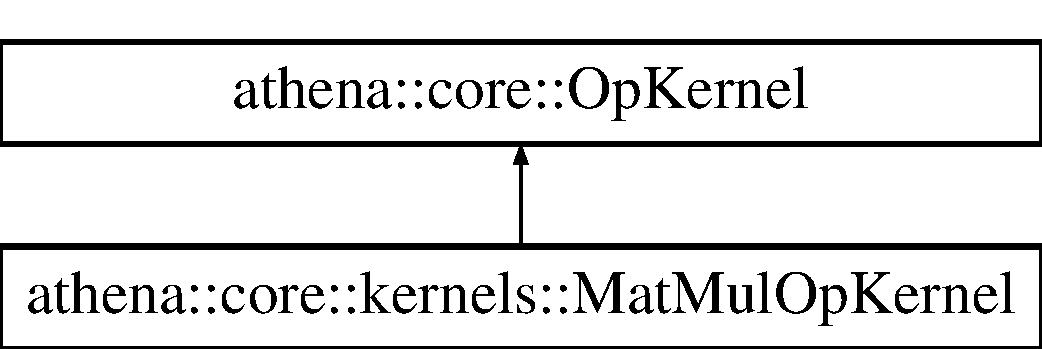
\includegraphics[height=2.000000cm]{db/dc5/classathena_1_1core_1_1kernels_1_1_mat_mul_op_kernel}
\end{center}
\end{figure}
\subsection*{Public Member Functions}
\begin{DoxyCompactItemize}
\item 
int \mbox{\hyperlink{classathena_1_1core_1_1kernels_1_1_mat_mul_op_kernel_a75f9e43d1fcecaf9260af31c68cd69db}{get\+Operands\+Count}} () override
\item 
\mbox{\hyperlink{classathena_1_1core_1_1_tensor_shape}{athena\+::core\+::\+Tensor\+Shape}} \& \mbox{\hyperlink{classathena_1_1core_1_1kernels_1_1_mat_mul_op_kernel_a3a397257c208f55ba5fba4018112a605}{get\+Output\+Shape}} (std\+::vector$<$ \mbox{\hyperlink{classathena_1_1core_1_1_tensor_shape}{athena\+::core\+::\+Tensor\+Shape}} $>$ \&shapes) override
\item 
\mbox{\hyperlink{classathena_1_1core_1_1_tensor_shape}{athena\+::core\+::\+Tensor\+Shape}} \& \mbox{\hyperlink{classathena_1_1core_1_1kernels_1_1_mat_mul_op_kernel_abdb57e6ce0d67ce6263e0716fed25243}{get\+Derivative\+Shape}} (int d, std\+::vector$<$ \mbox{\hyperlink{classathena_1_1core_1_1_tensor_shape}{athena\+::core\+::\+Tensor\+Shape}} $>$ \&shapes) override
\item 
\mbox{\Hypertarget{classathena_1_1core_1_1kernels_1_1_mat_mul_op_kernel_ac6dc778bb5313e5c567410fd5f217351}\label{classathena_1_1core_1_1kernels_1_1_mat_mul_op_kernel_ac6dc778bb5313e5c567410fd5f217351}} 
std\+::vector$<$ vm\+\_\+word $>$ {\bfseries get\+Op\+Bytecode} (std\+::vector$<$ vm\+\_\+word $>$ args, vm\+\_\+word result\+Cell) override
\item 
std\+::vector$<$ vm\+\_\+word $>$ \mbox{\hyperlink{classathena_1_1core_1_1kernels_1_1_mat_mul_op_kernel_a42d08b8004e8033e01988eb2392215c8}{get\+Derivative\+Bytecode}} (int d, std\+::vector$<$ vm\+\_\+word $>$ args, vm\+\_\+word result\+Cell) override
\end{DoxyCompactItemize}
\subsection*{Additional Inherited Members}


\subsection{Detailed Description}
Performs matrix multiplication of given Tensors. Matrix is a 2-\/D \mbox{\hyperlink{classathena_1_1core_1_1_tensor}{Tensor}}. The main restriction for this operation is that the number of columns for the first column must be equal to the number of rows for the second matrix. The reason to introduce this operation apart from \mbox{\hyperlink{classathena_1_1core_1_1_tensor}{Tensor}} product is that it is widely adopted by different acceleration mechanism (B\+L\+AS, cu\+B\+L\+AS, Accelerate Framework, etc) 

Definition at line 29 of file Mat\+Mul\+Op\+Kernel.\+h.



\subsection{Member Function Documentation}
\mbox{\Hypertarget{classathena_1_1core_1_1kernels_1_1_mat_mul_op_kernel_a42d08b8004e8033e01988eb2392215c8}\label{classathena_1_1core_1_1kernels_1_1_mat_mul_op_kernel_a42d08b8004e8033e01988eb2392215c8}} 
\index{athena\+::core\+::kernels\+::\+Mat\+Mul\+Op\+Kernel@{athena\+::core\+::kernels\+::\+Mat\+Mul\+Op\+Kernel}!get\+Derivative\+Bytecode@{get\+Derivative\+Bytecode}}
\index{get\+Derivative\+Bytecode@{get\+Derivative\+Bytecode}!athena\+::core\+::kernels\+::\+Mat\+Mul\+Op\+Kernel@{athena\+::core\+::kernels\+::\+Mat\+Mul\+Op\+Kernel}}
\subsubsection{\texorpdfstring{get\+Derivative\+Bytecode()}{getDerivativeBytecode()}}
{\footnotesize\ttfamily std\+::vector$<$ vm\+\_\+word $>$ athena\+::core\+::kernels\+::\+Mat\+Mul\+Op\+Kernel\+::get\+Derivative\+Bytecode (\begin{DoxyParamCaption}\item[{int}]{d,  }\item[{std\+::vector$<$ vm\+\_\+word $>$}]{args,  }\item[{vm\+\_\+word}]{result\+Cell }\end{DoxyParamCaption})\hspace{0.3cm}{\ttfamily [override]}, {\ttfamily [virtual]}}

Generates bytecode to calculate partial derivative 
\begin{DoxyParams}{Parameters}
{\em d} & Number of variable with respect to which derivative is calculated \\
\hline
{\em args} & Function arguments \\
\hline
{\em result\+Cell} & Number of memory cell where results are saved \\
\hline
\end{DoxyParams}
\begin{DoxyReturn}{Returns}

\end{DoxyReturn}


Implements \mbox{\hyperlink{classathena_1_1core_1_1_op_kernel_ad500db1afc5a7c10acff8ecb8f1bee4d}{athena\+::core\+::\+Op\+Kernel}}.



Definition at line 38 of file Mat\+Mul\+Op\+Kernel.\+cpp.

\mbox{\Hypertarget{classathena_1_1core_1_1kernels_1_1_mat_mul_op_kernel_abdb57e6ce0d67ce6263e0716fed25243}\label{classathena_1_1core_1_1kernels_1_1_mat_mul_op_kernel_abdb57e6ce0d67ce6263e0716fed25243}} 
\index{athena\+::core\+::kernels\+::\+Mat\+Mul\+Op\+Kernel@{athena\+::core\+::kernels\+::\+Mat\+Mul\+Op\+Kernel}!get\+Derivative\+Shape@{get\+Derivative\+Shape}}
\index{get\+Derivative\+Shape@{get\+Derivative\+Shape}!athena\+::core\+::kernels\+::\+Mat\+Mul\+Op\+Kernel@{athena\+::core\+::kernels\+::\+Mat\+Mul\+Op\+Kernel}}
\subsubsection{\texorpdfstring{get\+Derivative\+Shape()}{getDerivativeShape()}}
{\footnotesize\ttfamily \mbox{\hyperlink{classathena_1_1core_1_1_tensor_shape}{athena\+::core\+::\+Tensor\+Shape}} \& athena\+::core\+::kernels\+::\+Mat\+Mul\+Op\+Kernel\+::get\+Derivative\+Shape (\begin{DoxyParamCaption}\item[{int}]{d,  }\item[{std\+::vector$<$ \mbox{\hyperlink{classathena_1_1core_1_1_tensor_shape}{athena\+::core\+::\+Tensor\+Shape}} $>$ \&}]{shapes }\end{DoxyParamCaption})\hspace{0.3cm}{\ttfamily [override]}, {\ttfamily [virtual]}}

It is important for some operations to have certain size of their operands 
\begin{DoxyParams}{Parameters}
{\em shape} & Original operand shape \\
\hline
{\em dim} & Dimensionality \\
\hline
\end{DoxyParams}
\begin{DoxyReturn}{Returns}
New shape 
\end{DoxyReturn}


Implements \mbox{\hyperlink{classathena_1_1core_1_1_op_kernel_ad95af6dd184ce7ee9182ec7ca54b6c4d}{athena\+::core\+::\+Op\+Kernel}}.



Definition at line 63 of file Mat\+Mul\+Op\+Kernel.\+cpp.

\mbox{\Hypertarget{classathena_1_1core_1_1kernels_1_1_mat_mul_op_kernel_a75f9e43d1fcecaf9260af31c68cd69db}\label{classathena_1_1core_1_1kernels_1_1_mat_mul_op_kernel_a75f9e43d1fcecaf9260af31c68cd69db}} 
\index{athena\+::core\+::kernels\+::\+Mat\+Mul\+Op\+Kernel@{athena\+::core\+::kernels\+::\+Mat\+Mul\+Op\+Kernel}!get\+Operands\+Count@{get\+Operands\+Count}}
\index{get\+Operands\+Count@{get\+Operands\+Count}!athena\+::core\+::kernels\+::\+Mat\+Mul\+Op\+Kernel@{athena\+::core\+::kernels\+::\+Mat\+Mul\+Op\+Kernel}}
\subsubsection{\texorpdfstring{get\+Operands\+Count()}{getOperandsCount()}}
{\footnotesize\ttfamily int athena\+::core\+::kernels\+::\+Mat\+Mul\+Op\+Kernel\+::get\+Operands\+Count (\begin{DoxyParamCaption}{ }\end{DoxyParamCaption})\hspace{0.3cm}{\ttfamily [override]}, {\ttfamily [virtual]}}

There can be unary, binary and other operations \begin{DoxyReturn}{Returns}
Number of operands accepted 
\end{DoxyReturn}


Implements \mbox{\hyperlink{classathena_1_1core_1_1_op_kernel_add97d4c132d80ecd9915acfedf7c9119}{athena\+::core\+::\+Op\+Kernel}}.



Definition at line 16 of file Mat\+Mul\+Op\+Kernel.\+cpp.

\mbox{\Hypertarget{classathena_1_1core_1_1kernels_1_1_mat_mul_op_kernel_a3a397257c208f55ba5fba4018112a605}\label{classathena_1_1core_1_1kernels_1_1_mat_mul_op_kernel_a3a397257c208f55ba5fba4018112a605}} 
\index{athena\+::core\+::kernels\+::\+Mat\+Mul\+Op\+Kernel@{athena\+::core\+::kernels\+::\+Mat\+Mul\+Op\+Kernel}!get\+Output\+Shape@{get\+Output\+Shape}}
\index{get\+Output\+Shape@{get\+Output\+Shape}!athena\+::core\+::kernels\+::\+Mat\+Mul\+Op\+Kernel@{athena\+::core\+::kernels\+::\+Mat\+Mul\+Op\+Kernel}}
\subsubsection{\texorpdfstring{get\+Output\+Shape()}{getOutputShape()}}
{\footnotesize\ttfamily \mbox{\hyperlink{classathena_1_1core_1_1_tensor_shape}{athena\+::core\+::\+Tensor\+Shape}} \& athena\+::core\+::kernels\+::\+Mat\+Mul\+Op\+Kernel\+::get\+Output\+Shape (\begin{DoxyParamCaption}\item[{std\+::vector$<$ \mbox{\hyperlink{classathena_1_1core_1_1_tensor_shape}{athena\+::core\+::\+Tensor\+Shape}} $>$ \&}]{shapes }\end{DoxyParamCaption})\hspace{0.3cm}{\ttfamily [override]}, {\ttfamily [virtual]}}

It is important for some operations to have certain size of their operands 
\begin{DoxyParams}{Parameters}
{\em shape} & Original operand shape \\
\hline
{\em dim} & Dimensionality \\
\hline
\end{DoxyParams}
\begin{DoxyReturn}{Returns}
New shape 
\end{DoxyReturn}


Implements \mbox{\hyperlink{classathena_1_1core_1_1_op_kernel_a762e541463ffd089b47a8e6755c30fe1}{athena\+::core\+::\+Op\+Kernel}}.



Definition at line 56 of file Mat\+Mul\+Op\+Kernel.\+cpp.



The documentation for this class was generated from the following files\+:\begin{DoxyCompactItemize}
\item 
core/kernels/Mat\+Mul\+Op\+Kernel.\+h\item 
core/kernels/Mat\+Mul\+Op\+Kernel.\+cpp\end{DoxyCompactItemize}

\hypertarget{structathena_1_1backend_1_1generic_1_1_memory_chunk}{}\section{athena\+:\+:backend\+:\+:generic\+:\+:Memory\+Chunk Struct Reference}
\label{structathena_1_1backend_1_1generic_1_1_memory_chunk}\index{athena\+::backend\+::generic\+::\+Memory\+Chunk@{athena\+::backend\+::generic\+::\+Memory\+Chunk}}


{\ttfamily \#include $<$Generic\+Memory\+Manager.\+h$>$}

\subsection*{Public Attributes}
\begin{DoxyCompactItemize}
\item 
\mbox{\Hypertarget{structathena_1_1backend_1_1generic_1_1_memory_chunk_ad3c53eac117c1601d9305337e1a10fbf}\label{structathena_1_1backend_1_1generic_1_1_memory_chunk_ad3c53eac117c1601d9305337e1a10fbf}} 
vm\+\_\+word {\bfseries virtual\+Address}
\item 
\mbox{\Hypertarget{structathena_1_1backend_1_1generic_1_1_memory_chunk_aa9038ea35b158b4976da1991d9a219f8}\label{structathena_1_1backend_1_1generic_1_1_memory_chunk_aa9038ea35b158b4976da1991d9a219f8}} 
void $\ast$ {\bfseries begin}
\item 
\mbox{\Hypertarget{structathena_1_1backend_1_1generic_1_1_memory_chunk_a0b3f7644bb120bc1da34458cc4f51ad3}\label{structathena_1_1backend_1_1generic_1_1_memory_chunk_a0b3f7644bb120bc1da34458cc4f51ad3}} 
size\+\_\+t {\bfseries length}
\item 
\mbox{\Hypertarget{structathena_1_1backend_1_1generic_1_1_memory_chunk_a8f2afc822c82e708315e86744182dc4b}\label{structathena_1_1backend_1_1generic_1_1_memory_chunk_a8f2afc822c82e708315e86744182dc4b}} 
bool {\bfseries is\+Free}
\item 
\mbox{\Hypertarget{structathena_1_1backend_1_1generic_1_1_memory_chunk_abc625d2255dd2424fd9472ebb902558d}\label{structathena_1_1backend_1_1generic_1_1_memory_chunk_abc625d2255dd2424fd9472ebb902558d}} 
bool {\bfseries is\+Locked}
\item 
\mbox{\Hypertarget{structathena_1_1backend_1_1generic_1_1_memory_chunk_aa7ef44cb17321d0f3e1ff19779dd6ade}\label{structathena_1_1backend_1_1generic_1_1_memory_chunk_aa7ef44cb17321d0f3e1ff19779dd6ade}} 
\mbox{\hyperlink{structathena_1_1backend_1_1generic_1_1_memory_chunk}{Memory\+Chunk}} $\ast$ {\bfseries next}
\item 
\mbox{\Hypertarget{structathena_1_1backend_1_1generic_1_1_memory_chunk_ad61468f9a985ba872f81dc8526fc5c23}\label{structathena_1_1backend_1_1generic_1_1_memory_chunk_ad61468f9a985ba872f81dc8526fc5c23}} 
\mbox{\hyperlink{structathena_1_1backend_1_1generic_1_1_memory_chunk}{Memory\+Chunk}} $\ast$ {\bfseries prev}
\end{DoxyCompactItemize}


\subsection{Detailed Description}
Describes single memory chunk that is allocated in R\+AM. Free status means there is no data in this chunk Locked status means this chunk is being used now and can\textquotesingle{}t be unload to persistent memory. 

Definition at line 46 of file Generic\+Memory\+Manager.\+h.



The documentation for this struct was generated from the following file\+:\begin{DoxyCompactItemize}
\item 
backend/generic/Generic\+Memory\+Manager.\+h\end{DoxyCompactItemize}

\hypertarget{classathena_1_1core_1_1loss_1_1_m_s_e_loss}{}\section{athena\+:\+:core\+:\+:loss\+:\+:M\+S\+E\+Loss Class Reference}
\label{classathena_1_1core_1_1loss_1_1_m_s_e_loss}\index{athena\+::core\+::loss\+::\+M\+S\+E\+Loss@{athena\+::core\+::loss\+::\+M\+S\+E\+Loss}}
Inheritance diagram for athena\+:\+:core\+:\+:loss\+:\+:M\+S\+E\+Loss\+:\begin{figure}[H]
\begin{center}
\leavevmode
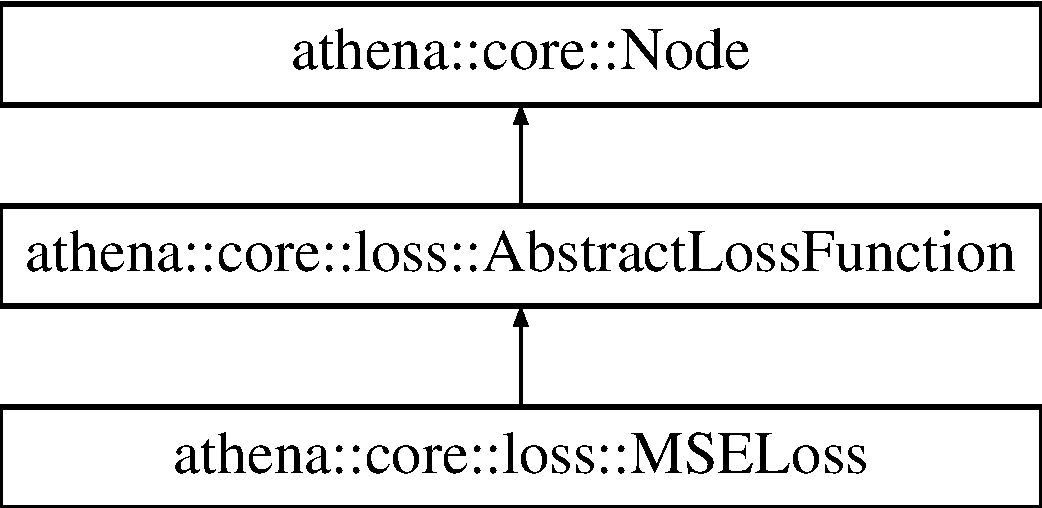
\includegraphics[height=3.000000cm]{dc/d9a/classathena_1_1core_1_1loss_1_1_m_s_e_loss}
\end{center}
\end{figure}
\subsection*{Additional Inherited Members}


\subsection{Detailed Description}


Definition at line 38 of file M\+S\+E\+Loss.\+h.



The documentation for this class was generated from the following files\+:\begin{DoxyCompactItemize}
\item 
core/loss/M\+S\+E\+Loss.\+h\item 
core/loss/M\+S\+E\+Loss.\+cpp\end{DoxyCompactItemize}

\hypertarget{classathena_1_1core_1_1loss_1_1_m_s_e_op_kernel}{}\section{athena\+:\+:core\+:\+:loss\+:\+:M\+S\+E\+Op\+Kernel Class Reference}
\label{classathena_1_1core_1_1loss_1_1_m_s_e_op_kernel}\index{athena\+::core\+::loss\+::\+M\+S\+E\+Op\+Kernel@{athena\+::core\+::loss\+::\+M\+S\+E\+Op\+Kernel}}
Inheritance diagram for athena\+:\+:core\+:\+:loss\+:\+:M\+S\+E\+Op\+Kernel\+:\begin{figure}[H]
\begin{center}
\leavevmode
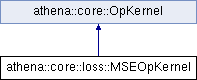
\includegraphics[height=2.000000cm]{df/d1d/classathena_1_1core_1_1loss_1_1_m_s_e_op_kernel}
\end{center}
\end{figure}
\subsection*{Public Member Functions}
\begin{DoxyCompactItemize}
\item 
int \mbox{\hyperlink{classathena_1_1core_1_1loss_1_1_m_s_e_op_kernel_ab851ee62ea95c3aab8aab2d28cfa9d04}{get\+Operands\+Count}} () override
\item 
\mbox{\hyperlink{classathena_1_1core_1_1_tensor_shape}{athena\+::core\+::\+Tensor\+Shape}} \& \mbox{\hyperlink{classathena_1_1core_1_1loss_1_1_m_s_e_op_kernel_a23aacffbbc73b177535511702f3c441d}{get\+Output\+Shape}} (std\+::vector$<$ \mbox{\hyperlink{classathena_1_1core_1_1_tensor_shape}{athena\+::core\+::\+Tensor\+Shape}} $>$ \&shapes) override
\item 
\mbox{\hyperlink{classathena_1_1core_1_1_tensor_shape}{athena\+::core\+::\+Tensor\+Shape}} \& \mbox{\hyperlink{classathena_1_1core_1_1loss_1_1_m_s_e_op_kernel_a68a0220e3a3591638c7725b5cb659609}{get\+Derivative\+Shape}} (int, std\+::vector$<$ \mbox{\hyperlink{classathena_1_1core_1_1_tensor_shape}{athena\+::core\+::\+Tensor\+Shape}} $>$ \&shapes) override
\item 
\mbox{\Hypertarget{classathena_1_1core_1_1loss_1_1_m_s_e_op_kernel_a92d3c2ca58c2a67df6dbf623c5d1ce65}\label{classathena_1_1core_1_1loss_1_1_m_s_e_op_kernel_a92d3c2ca58c2a67df6dbf623c5d1ce65}} 
std\+::vector$<$ vm\+\_\+word $>$ {\bfseries get\+Op\+Bytecode} (std\+::vector$<$ vm\+\_\+word $>$ args, vm\+\_\+word result\+Cell) override
\item 
std\+::vector$<$ vm\+\_\+word $>$ \mbox{\hyperlink{classathena_1_1core_1_1loss_1_1_m_s_e_op_kernel_a936002563d3ef3a029bbeecbdbd3a509}{get\+Derivative\+Bytecode}} (int d, std\+::vector$<$ vm\+\_\+word $>$ args, vm\+\_\+word result\+Cell) override
\end{DoxyCompactItemize}
\subsection*{Additional Inherited Members}


\subsection{Detailed Description}


Definition at line 22 of file M\+S\+E\+Loss.\+h.



\subsection{Member Function Documentation}
\mbox{\Hypertarget{classathena_1_1core_1_1loss_1_1_m_s_e_op_kernel_a936002563d3ef3a029bbeecbdbd3a509}\label{classathena_1_1core_1_1loss_1_1_m_s_e_op_kernel_a936002563d3ef3a029bbeecbdbd3a509}} 
\index{athena\+::core\+::loss\+::\+M\+S\+E\+Op\+Kernel@{athena\+::core\+::loss\+::\+M\+S\+E\+Op\+Kernel}!get\+Derivative\+Bytecode@{get\+Derivative\+Bytecode}}
\index{get\+Derivative\+Bytecode@{get\+Derivative\+Bytecode}!athena\+::core\+::loss\+::\+M\+S\+E\+Op\+Kernel@{athena\+::core\+::loss\+::\+M\+S\+E\+Op\+Kernel}}
\subsubsection{\texorpdfstring{get\+Derivative\+Bytecode()}{getDerivativeBytecode()}}
{\footnotesize\ttfamily std\+::vector$<$ vm\+\_\+word $>$ athena\+::core\+::loss\+::\+M\+S\+E\+Op\+Kernel\+::get\+Derivative\+Bytecode (\begin{DoxyParamCaption}\item[{int}]{d,  }\item[{std\+::vector$<$ vm\+\_\+word $>$}]{args,  }\item[{vm\+\_\+word}]{result\+Cell }\end{DoxyParamCaption})\hspace{0.3cm}{\ttfamily [override]}, {\ttfamily [virtual]}}

Generates bytecode to calculate partial derivative 
\begin{DoxyParams}{Parameters}
{\em d} & Number of variable with respect to which derivative is calculated \\
\hline
{\em args} & Function arguments \\
\hline
{\em result\+Cell} & Number of memory cell where results are saved \\
\hline
\end{DoxyParams}
\begin{DoxyReturn}{Returns}

\end{DoxyReturn}


Implements \mbox{\hyperlink{classathena_1_1core_1_1_op_kernel_ad500db1afc5a7c10acff8ecb8f1bee4d}{athena\+::core\+::\+Op\+Kernel}}.



Definition at line 40 of file M\+S\+E\+Loss.\+cpp.

\mbox{\Hypertarget{classathena_1_1core_1_1loss_1_1_m_s_e_op_kernel_a68a0220e3a3591638c7725b5cb659609}\label{classathena_1_1core_1_1loss_1_1_m_s_e_op_kernel_a68a0220e3a3591638c7725b5cb659609}} 
\index{athena\+::core\+::loss\+::\+M\+S\+E\+Op\+Kernel@{athena\+::core\+::loss\+::\+M\+S\+E\+Op\+Kernel}!get\+Derivative\+Shape@{get\+Derivative\+Shape}}
\index{get\+Derivative\+Shape@{get\+Derivative\+Shape}!athena\+::core\+::loss\+::\+M\+S\+E\+Op\+Kernel@{athena\+::core\+::loss\+::\+M\+S\+E\+Op\+Kernel}}
\subsubsection{\texorpdfstring{get\+Derivative\+Shape()}{getDerivativeShape()}}
{\footnotesize\ttfamily \mbox{\hyperlink{classathena_1_1core_1_1_tensor_shape}{athena\+::core\+::\+Tensor\+Shape}} \& athena\+::core\+::loss\+::\+M\+S\+E\+Op\+Kernel\+::get\+Derivative\+Shape (\begin{DoxyParamCaption}\item[{int}]{d,  }\item[{std\+::vector$<$ \mbox{\hyperlink{classathena_1_1core_1_1_tensor_shape}{athena\+::core\+::\+Tensor\+Shape}} $>$ \&}]{shapes }\end{DoxyParamCaption})\hspace{0.3cm}{\ttfamily [override]}, {\ttfamily [virtual]}}

It is important for some operations to have certain size of their operands 
\begin{DoxyParams}{Parameters}
{\em shape} & Original operand shape \\
\hline
{\em dim} & Dimensionality \\
\hline
\end{DoxyParams}
\begin{DoxyReturn}{Returns}
New shape 
\end{DoxyReturn}


Implements \mbox{\hyperlink{classathena_1_1core_1_1_op_kernel_ad95af6dd184ce7ee9182ec7ca54b6c4d}{athena\+::core\+::\+Op\+Kernel}}.



Definition at line 59 of file M\+S\+E\+Loss.\+cpp.

\mbox{\Hypertarget{classathena_1_1core_1_1loss_1_1_m_s_e_op_kernel_ab851ee62ea95c3aab8aab2d28cfa9d04}\label{classathena_1_1core_1_1loss_1_1_m_s_e_op_kernel_ab851ee62ea95c3aab8aab2d28cfa9d04}} 
\index{athena\+::core\+::loss\+::\+M\+S\+E\+Op\+Kernel@{athena\+::core\+::loss\+::\+M\+S\+E\+Op\+Kernel}!get\+Operands\+Count@{get\+Operands\+Count}}
\index{get\+Operands\+Count@{get\+Operands\+Count}!athena\+::core\+::loss\+::\+M\+S\+E\+Op\+Kernel@{athena\+::core\+::loss\+::\+M\+S\+E\+Op\+Kernel}}
\subsubsection{\texorpdfstring{get\+Operands\+Count()}{getOperandsCount()}}
{\footnotesize\ttfamily int athena\+::core\+::loss\+::\+M\+S\+E\+Op\+Kernel\+::get\+Operands\+Count (\begin{DoxyParamCaption}{ }\end{DoxyParamCaption})\hspace{0.3cm}{\ttfamily [override]}, {\ttfamily [virtual]}}

There can be unary, binary and other operations \begin{DoxyReturn}{Returns}
Number of operands accepted 
\end{DoxyReturn}


Implements \mbox{\hyperlink{classathena_1_1core_1_1_op_kernel_add97d4c132d80ecd9915acfedf7c9119}{athena\+::core\+::\+Op\+Kernel}}.



Definition at line 22 of file M\+S\+E\+Loss.\+cpp.

\mbox{\Hypertarget{classathena_1_1core_1_1loss_1_1_m_s_e_op_kernel_a23aacffbbc73b177535511702f3c441d}\label{classathena_1_1core_1_1loss_1_1_m_s_e_op_kernel_a23aacffbbc73b177535511702f3c441d}} 
\index{athena\+::core\+::loss\+::\+M\+S\+E\+Op\+Kernel@{athena\+::core\+::loss\+::\+M\+S\+E\+Op\+Kernel}!get\+Output\+Shape@{get\+Output\+Shape}}
\index{get\+Output\+Shape@{get\+Output\+Shape}!athena\+::core\+::loss\+::\+M\+S\+E\+Op\+Kernel@{athena\+::core\+::loss\+::\+M\+S\+E\+Op\+Kernel}}
\subsubsection{\texorpdfstring{get\+Output\+Shape()}{getOutputShape()}}
{\footnotesize\ttfamily \mbox{\hyperlink{classathena_1_1core_1_1_tensor_shape}{athena\+::core\+::\+Tensor\+Shape}} \& athena\+::core\+::loss\+::\+M\+S\+E\+Op\+Kernel\+::get\+Output\+Shape (\begin{DoxyParamCaption}\item[{std\+::vector$<$ \mbox{\hyperlink{classathena_1_1core_1_1_tensor_shape}{athena\+::core\+::\+Tensor\+Shape}} $>$ \&}]{shapes }\end{DoxyParamCaption})\hspace{0.3cm}{\ttfamily [override]}, {\ttfamily [virtual]}}

It is important for some operations to have certain size of their operands 
\begin{DoxyParams}{Parameters}
{\em shape} & Original operand shape \\
\hline
{\em dim} & Dimensionality \\
\hline
\end{DoxyParams}
\begin{DoxyReturn}{Returns}
New shape 
\end{DoxyReturn}


Implements \mbox{\hyperlink{classathena_1_1core_1_1_op_kernel_a762e541463ffd089b47a8e6755c30fe1}{athena\+::core\+::\+Op\+Kernel}}.



Definition at line 53 of file M\+S\+E\+Loss.\+cpp.



The documentation for this class was generated from the following files\+:\begin{DoxyCompactItemize}
\item 
core/loss/M\+S\+E\+Loss.\+h\item 
core/loss/M\+S\+E\+Loss.\+cpp\end{DoxyCompactItemize}

\hypertarget{classathena_1_1core_1_1_node}{}\section{athena\+:\+:core\+:\+:Node Class Reference}
\label{classathena_1_1core_1_1_node}\index{athena\+::core\+::\+Node@{athena\+::core\+::\+Node}}


{\ttfamily \#include $<$Node.\+h$>$}

Inheritance diagram for athena\+:\+:core\+:\+:Node\+:\begin{figure}[H]
\begin{center}
\leavevmode
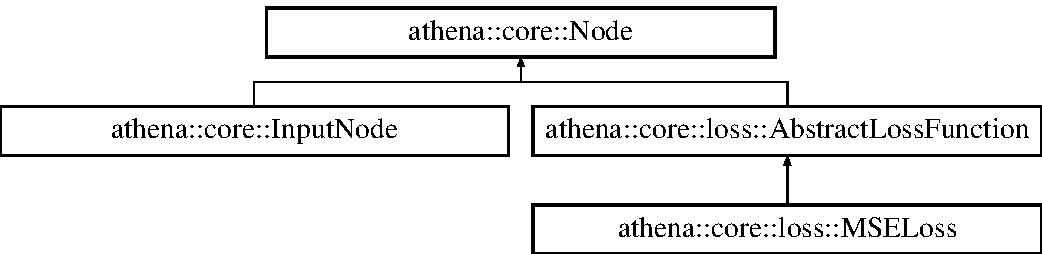
\includegraphics[height=3.000000cm]{d9/dbb/classathena_1_1core_1_1_node}
\end{center}
\end{figure}
\subsection*{Public Member Functions}
\begin{DoxyCompactItemize}
\item 
\mbox{\Hypertarget{classathena_1_1core_1_1_node_a7c8ca7c16db4d9d55b2ea3f4336e73ec}\label{classathena_1_1core_1_1_node_a7c8ca7c16db4d9d55b2ea3f4336e73ec}} 
{\bfseries Node} (\mbox{\hyperlink{classathena_1_1core_1_1_op_kernel}{Op\+Kernel}} $\ast$)
\item 
virtual void \mbox{\hyperlink{classathena_1_1core_1_1_node_aefef588463c8e215e998415a7cc6b320}{after}} (\mbox{\hyperlink{classathena_1_1core_1_1_node}{Node}} $\ast$predecessor)
\item 
virtual bool \mbox{\hyperlink{classathena_1_1core_1_1_node_a6ae012557fc6b29127366b1e92801d4a}{is\+Input\+Node}} ()
\item 
\mbox{\Hypertarget{classathena_1_1core_1_1_node_a185a846d26ff9e8bbe21c03ce32aca47}\label{classathena_1_1core_1_1_node_a185a846d26ff9e8bbe21c03ce32aca47}} 
\mbox{\hyperlink{classathena_1_1core_1_1_op_kernel}{Op\+Kernel}} $\ast$ {\bfseries get\+Op} ()
\item 
\mbox{\Hypertarget{classathena_1_1core_1_1_node_ae4e0e34ffc5d79c5a18d33847cc80331}\label{classathena_1_1core_1_1_node_ae4e0e34ffc5d79c5a18d33847cc80331}} 
std\+::vector$<$ \mbox{\hyperlink{classathena_1_1core_1_1_node}{Node}} $\ast$$>$ \& {\bfseries get\+Incoming\+Nodes} ()
\item 
\mbox{\Hypertarget{classathena_1_1core_1_1_node_a28043abbb7dc60c6a510839928fa2408}\label{classathena_1_1core_1_1_node_a28043abbb7dc60c6a510839928fa2408}} 
std\+::string {\bfseries get\+Name} ()
\item 
\mbox{\Hypertarget{classathena_1_1core_1_1_node_a290e21f4231f4193c2877b8b85c1864a}\label{classathena_1_1core_1_1_node_a290e21f4231f4193c2877b8b85c1864a}} 
void {\bfseries add\+Derivative} (unsigned long d)
\item 
\mbox{\Hypertarget{classathena_1_1core_1_1_node_a5f737753ebd25e521c0ac8a995ca7625}\label{classathena_1_1core_1_1_node_a5f737753ebd25e521c0ac8a995ca7625}} 
unsigned long {\bfseries get\+Derivative} (int i)
\item 
\mbox{\Hypertarget{classathena_1_1core_1_1_node_af0d6ae48f88c47a04c592c71c4b119e7}\label{classathena_1_1core_1_1_node_af0d6ae48f88c47a04c592c71c4b119e7}} 
void {\bfseries set\+Calculated} (unsigned long res\+Cell)
\item 
\mbox{\Hypertarget{classathena_1_1core_1_1_node_af75ed35cf7ec81f686292b1cef4c549d}\label{classathena_1_1core_1_1_node_af75ed35cf7ec81f686292b1cef4c549d}} 
bool {\bfseries is\+Calculated} ()
\item 
\mbox{\Hypertarget{classathena_1_1core_1_1_node_ae2568f40260ef891d79618c16d2fc1a8}\label{classathena_1_1core_1_1_node_ae2568f40260ef891d79618c16d2fc1a8}} 
unsigned long {\bfseries get\+Result} ()
\item 
\mbox{\Hypertarget{classathena_1_1core_1_1_node_ae160501f8419f9874bd71aefe6daa3dc}\label{classathena_1_1core_1_1_node_ae160501f8419f9874bd71aefe6daa3dc}} 
void {\bfseries update\+Usage\+Count} ()
\item 
\mbox{\Hypertarget{classathena_1_1core_1_1_node_ad0e6344fe6940e59d79eb4b05a7a5b96}\label{classathena_1_1core_1_1_node_ad0e6344fe6940e59d79eb4b05a7a5b96}} 
bool {\bfseries is\+Garbage} ()
\end{DoxyCompactItemize}
\subsection*{Protected Member Functions}
\begin{DoxyCompactItemize}
\item 
\mbox{\Hypertarget{classathena_1_1core_1_1_node_aa2aee4b3d80299df55739295d8f7040a}\label{classathena_1_1core_1_1_node_aa2aee4b3d80299df55739295d8f7040a}} 
std\+::string {\bfseries get\+Random\+Node\+Name} ()
\end{DoxyCompactItemize}
\subsection*{Protected Attributes}
\begin{DoxyCompactItemize}
\item 
\mbox{\Hypertarget{classathena_1_1core_1_1_node_aa46df2cfca5ac1bb88d683e52614397e}\label{classathena_1_1core_1_1_node_aa46df2cfca5ac1bb88d683e52614397e}} 
std\+::vector$<$ \mbox{\hyperlink{classathena_1_1core_1_1_node}{Node}} $\ast$$>$ {\bfseries incoming\+Nodes}
\item 
\mbox{\Hypertarget{classathena_1_1core_1_1_node_a156010639b24e35c17cbe15de5078bbb}\label{classathena_1_1core_1_1_node_a156010639b24e35c17cbe15de5078bbb}} 
std\+::vector$<$ \mbox{\hyperlink{classathena_1_1core_1_1_node}{Node}} $\ast$$>$ {\bfseries outcoming\+Nodes}
\item 
\mbox{\Hypertarget{classathena_1_1core_1_1_node_a27276034dd9d663c195e6233d32013be}\label{classathena_1_1core_1_1_node_a27276034dd9d663c195e6233d32013be}} 
\mbox{\hyperlink{classathena_1_1core_1_1_op_kernel}{Op\+Kernel}} $\ast$ {\bfseries operation}
\item 
\mbox{\Hypertarget{classathena_1_1core_1_1_node_a4f2c3e1d4c44cf45bfa78909d4df3777}\label{classathena_1_1core_1_1_node_a4f2c3e1d4c44cf45bfa78909d4df3777}} 
std\+::string {\bfseries name}
\item 
\mbox{\Hypertarget{classathena_1_1core_1_1_node_a9b66b2c502174ec4253540e785ed65d1}\label{classathena_1_1core_1_1_node_a9b66b2c502174ec4253540e785ed65d1}} 
bool {\bfseries calculated}
\item 
\mbox{\Hypertarget{classathena_1_1core_1_1_node_a753a10d861a9e65c0ceac674a64f93b2}\label{classathena_1_1core_1_1_node_a753a10d861a9e65c0ceac674a64f93b2}} 
std\+::vector$<$ vm\+\_\+word $>$ {\bfseries derivatives}
\item 
\mbox{\Hypertarget{classathena_1_1core_1_1_node_a3b79e7b88f22fac99cca9323bd2fb644}\label{classathena_1_1core_1_1_node_a3b79e7b88f22fac99cca9323bd2fb644}} 
unsigned long {\bfseries result\+Cell}
\item 
\mbox{\Hypertarget{classathena_1_1core_1_1_node_ad8f1fef6f146b1fcc73b9333a5dc3fa0}\label{classathena_1_1core_1_1_node_ad8f1fef6f146b1fcc73b9333a5dc3fa0}} 
unsigned long {\bfseries usage\+Count}
\item 
\mbox{\Hypertarget{classathena_1_1core_1_1_node_ad04d91c676f72a3e91e77486513e5080}\label{classathena_1_1core_1_1_node_ad04d91c676f72a3e91e77486513e5080}} 
bool {\bfseries derivative\+Mark}
\end{DoxyCompactItemize}


\subsection{Detailed Description}
A basic element of execution graph Each node has pointers to its predecessors and successors. It encapsulates operation and data. 

Definition at line 16 of file Node.\+h.



\subsection{Member Function Documentation}
\mbox{\Hypertarget{classathena_1_1core_1_1_node_aefef588463c8e215e998415a7cc6b320}\label{classathena_1_1core_1_1_node_aefef588463c8e215e998415a7cc6b320}} 
\index{athena\+::core\+::\+Node@{athena\+::core\+::\+Node}!after@{after}}
\index{after@{after}!athena\+::core\+::\+Node@{athena\+::core\+::\+Node}}
\subsubsection{\texorpdfstring{after()}{after()}}
{\footnotesize\ttfamily void athena\+::core\+::\+Node\+::after (\begin{DoxyParamCaption}\item[{\mbox{\hyperlink{classathena_1_1core_1_1_node}{Node}} $\ast$}]{predecessor }\end{DoxyParamCaption})\hspace{0.3cm}{\ttfamily [virtual]}}

Makes a new oriented edge in execution graph from predecessor to this node 
\begin{DoxyParams}{Parameters}
{\em predecessor} & A predecessor node \\
\hline
\end{DoxyParams}


Reimplemented in \mbox{\hyperlink{classathena_1_1core_1_1_input_node_aaec12f4c76b6d9890efe1fb4337a1b61}{athena\+::core\+::\+Input\+Node}}.



Definition at line 13 of file Node.\+cpp.

\mbox{\Hypertarget{classathena_1_1core_1_1_node_a6ae012557fc6b29127366b1e92801d4a}\label{classathena_1_1core_1_1_node_a6ae012557fc6b29127366b1e92801d4a}} 
\index{athena\+::core\+::\+Node@{athena\+::core\+::\+Node}!is\+Input\+Node@{is\+Input\+Node}}
\index{is\+Input\+Node@{is\+Input\+Node}!athena\+::core\+::\+Node@{athena\+::core\+::\+Node}}
\subsubsection{\texorpdfstring{is\+Input\+Node()}{isInputNode()}}
{\footnotesize\ttfamily bool athena\+::core\+::\+Node\+::is\+Input\+Node (\begin{DoxyParamCaption}{ }\end{DoxyParamCaption})\hspace{0.3cm}{\ttfamily [virtual]}}

Check if it is an input node \begin{DoxyReturn}{Returns}
false 
\end{DoxyReturn}


Reimplemented in \mbox{\hyperlink{classathena_1_1core_1_1_input_node_a2548b569a336b75c0005295833052979}{athena\+::core\+::\+Input\+Node}}.



Definition at line 24 of file Node.\+cpp.



The documentation for this class was generated from the following files\+:\begin{DoxyCompactItemize}
\item 
core/Node.\+h\item 
core/Node.\+cpp\end{DoxyCompactItemize}

\hypertarget{classathena_1_1core_1_1_op_kernel}{}\section{athena\+:\+:core\+:\+:Op\+Kernel Class Reference}
\label{classathena_1_1core_1_1_op_kernel}\index{athena\+::core\+::\+Op\+Kernel@{athena\+::core\+::\+Op\+Kernel}}


{\ttfamily \#include $<$Op\+Kernel.\+h$>$}

Inheritance diagram for athena\+:\+:core\+:\+:Op\+Kernel\+:\begin{figure}[H]
\begin{center}
\leavevmode
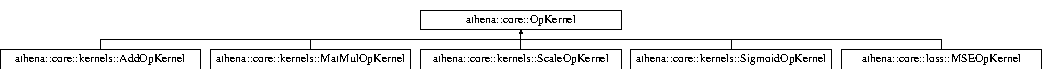
\includegraphics[height=0.929461cm]{classathena_1_1core_1_1_op_kernel}
\end{center}
\end{figure}
\subsection*{Public Member Functions}
\begin{DoxyCompactItemize}
\item 
\mbox{\Hypertarget{classathena_1_1core_1_1_op_kernel_a1adf0c5c97ce4d3e9c0155ea4bf48ab5}\label{classathena_1_1core_1_1_op_kernel_a1adf0c5c97ce4d3e9c0155ea4bf48ab5}} 
{\bfseries Op\+Kernel} (Op\+Code op\+Code, std\+::string name)
\item 
virtual int \mbox{\hyperlink{classathena_1_1core_1_1_op_kernel_add97d4c132d80ecd9915acfedf7c9119}{get\+Operands\+Count}} ()=0
\item 
virtual \mbox{\hyperlink{classathena_1_1core_1_1_tensor_shape}{athena\+::core\+::\+Tensor\+Shape}} \& \mbox{\hyperlink{classathena_1_1core_1_1_op_kernel_a762e541463ffd089b47a8e6755c30fe1}{get\+Output\+Shape}} (std\+::vector$<$ \mbox{\hyperlink{classathena_1_1core_1_1_tensor_shape}{athena\+::core\+::\+Tensor\+Shape}} $>$ \&shapes)=0
\item 
virtual \mbox{\hyperlink{classathena_1_1core_1_1_tensor_shape}{athena\+::core\+::\+Tensor\+Shape}} \& \mbox{\hyperlink{classathena_1_1core_1_1_op_kernel_ad95af6dd184ce7ee9182ec7ca54b6c4d}{get\+Derivative\+Shape}} (int d, std\+::vector$<$ \mbox{\hyperlink{classathena_1_1core_1_1_tensor_shape}{athena\+::core\+::\+Tensor\+Shape}} $>$ \&shapes)=0
\item 
\mbox{\Hypertarget{classathena_1_1core_1_1_op_kernel_a181a03e0a038151fda074a8c950f3003}\label{classathena_1_1core_1_1_op_kernel_a181a03e0a038151fda074a8c950f3003}} 
virtual std\+::vector$<$ vm\+\_\+word $>$ {\bfseries get\+Op\+Bytecode} (std\+::vector$<$ vm\+\_\+word $>$ args, vm\+\_\+word result\+Cell)=0
\item 
virtual std\+::vector$<$ vm\+\_\+word $>$ \mbox{\hyperlink{classathena_1_1core_1_1_op_kernel_ad500db1afc5a7c10acff8ecb8f1bee4d}{get\+Derivative\+Bytecode}} (int d, std\+::vector$<$ vm\+\_\+word $>$ args, vm\+\_\+word result\+Cell)=0
\end{DoxyCompactItemize}
\subsection*{Protected Attributes}
\begin{DoxyCompactItemize}
\item 
\mbox{\Hypertarget{classathena_1_1core_1_1_op_kernel_ae77be87c4209176d927a6d83bcbf3592}\label{classathena_1_1core_1_1_op_kernel_ae77be87c4209176d927a6d83bcbf3592}} 
Op\+Code {\bfseries op\+Code}
\item 
\mbox{\Hypertarget{classathena_1_1core_1_1_op_kernel_a5970ac8cb25cd956112a471d647789be}\label{classathena_1_1core_1_1_op_kernel_a5970ac8cb25cd956112a471d647789be}} 
std\+::string {\bfseries name}
\end{DoxyCompactItemize}


\subsection{Detailed Description}
Operation skeleton Each operation has Op\+Code 

\subsection{Member Function Documentation}
\mbox{\Hypertarget{classathena_1_1core_1_1_op_kernel_ad500db1afc5a7c10acff8ecb8f1bee4d}\label{classathena_1_1core_1_1_op_kernel_ad500db1afc5a7c10acff8ecb8f1bee4d}} 
\index{athena\+::core\+::\+Op\+Kernel@{athena\+::core\+::\+Op\+Kernel}!get\+Derivative\+Bytecode@{get\+Derivative\+Bytecode}}
\index{get\+Derivative\+Bytecode@{get\+Derivative\+Bytecode}!athena\+::core\+::\+Op\+Kernel@{athena\+::core\+::\+Op\+Kernel}}
\subsubsection{\texorpdfstring{get\+Derivative\+Bytecode()}{getDerivativeBytecode()}}
{\footnotesize\ttfamily virtual std\+::vector$<$ vm\+\_\+word $>$ athena\+::core\+::\+Op\+Kernel\+::get\+Derivative\+Bytecode (\begin{DoxyParamCaption}\item[{int}]{d,  }\item[{std\+::vector$<$ vm\+\_\+word $>$}]{args,  }\item[{vm\+\_\+word}]{result\+Cell }\end{DoxyParamCaption})\hspace{0.3cm}{\ttfamily [pure virtual]}}

Generates bytecode to calculate partial derivative 
\begin{DoxyParams}{Parameters}
{\em d} & Number of variable with respect to which derivative is calculated \\
\hline
{\em args} & Function arguments \\
\hline
{\em result\+Cell} & Number of memory cell where results are saved \\
\hline
\end{DoxyParams}
\begin{DoxyReturn}{Returns}

\end{DoxyReturn}


Implemented in \mbox{\hyperlink{classathena_1_1core_1_1kernels_1_1_mat_mul_op_kernel_a42d08b8004e8033e01988eb2392215c8}{athena\+::core\+::kernels\+::\+Mat\+Mul\+Op\+Kernel}}, \mbox{\hyperlink{classathena_1_1core_1_1kernels_1_1_sigmoid_op_kernel_a38166ae2204692353efa2f6270714a80}{athena\+::core\+::kernels\+::\+Sigmoid\+Op\+Kernel}}, \mbox{\hyperlink{classathena_1_1core_1_1loss_1_1_m_s_e_op_kernel_a2d1fc6b2900abc3ebd0466c8de3e68e2}{athena\+::core\+::loss\+::\+M\+S\+E\+Op\+Kernel}}, \mbox{\hyperlink{classathena_1_1core_1_1kernels_1_1_add_op_kernel_a97ac0c3c61c772563221c3148d553841}{athena\+::core\+::kernels\+::\+Add\+Op\+Kernel}}, and \mbox{\hyperlink{classathena_1_1core_1_1kernels_1_1_scale_op_kernel_ad35869239968db73049161acbad05aab}{athena\+::core\+::kernels\+::\+Scale\+Op\+Kernel}}.

\mbox{\Hypertarget{classathena_1_1core_1_1_op_kernel_ad95af6dd184ce7ee9182ec7ca54b6c4d}\label{classathena_1_1core_1_1_op_kernel_ad95af6dd184ce7ee9182ec7ca54b6c4d}} 
\index{athena\+::core\+::\+Op\+Kernel@{athena\+::core\+::\+Op\+Kernel}!get\+Derivative\+Shape@{get\+Derivative\+Shape}}
\index{get\+Derivative\+Shape@{get\+Derivative\+Shape}!athena\+::core\+::\+Op\+Kernel@{athena\+::core\+::\+Op\+Kernel}}
\subsubsection{\texorpdfstring{get\+Derivative\+Shape()}{getDerivativeShape()}}
{\footnotesize\ttfamily virtual \mbox{\hyperlink{classathena_1_1core_1_1_tensor_shape}{athena\+::core\+::\+Tensor\+Shape}}\& athena\+::core\+::\+Op\+Kernel\+::get\+Derivative\+Shape (\begin{DoxyParamCaption}\item[{int}]{d,  }\item[{std\+::vector$<$ \mbox{\hyperlink{classathena_1_1core_1_1_tensor_shape}{athena\+::core\+::\+Tensor\+Shape}} $>$ \&}]{shapes }\end{DoxyParamCaption})\hspace{0.3cm}{\ttfamily [pure virtual]}}

It is important for some operations to have certain size of their operands 
\begin{DoxyParams}{Parameters}
{\em shape} & Original operand shape \\
\hline
{\em dim} & Dimensionality \\
\hline
\end{DoxyParams}
\begin{DoxyReturn}{Returns}
New shape 
\end{DoxyReturn}


Implemented in \mbox{\hyperlink{classathena_1_1core_1_1kernels_1_1_mat_mul_op_kernel_abdb57e6ce0d67ce6263e0716fed25243}{athena\+::core\+::kernels\+::\+Mat\+Mul\+Op\+Kernel}}, \mbox{\hyperlink{classathena_1_1core_1_1kernels_1_1_sigmoid_op_kernel_a0ea18b43eb9355d7a855202898ff09fc}{athena\+::core\+::kernels\+::\+Sigmoid\+Op\+Kernel}}, \mbox{\hyperlink{classathena_1_1core_1_1loss_1_1_m_s_e_op_kernel_a68a0220e3a3591638c7725b5cb659609}{athena\+::core\+::loss\+::\+M\+S\+E\+Op\+Kernel}}, \mbox{\hyperlink{classathena_1_1core_1_1kernels_1_1_add_op_kernel_a240d13047b8fd7676bf1f9d2bc94298f}{athena\+::core\+::kernels\+::\+Add\+Op\+Kernel}}, and \mbox{\hyperlink{classathena_1_1core_1_1kernels_1_1_scale_op_kernel_ad7c63973c62e28c0ad3d854ce16debf1}{athena\+::core\+::kernels\+::\+Scale\+Op\+Kernel}}.

\mbox{\Hypertarget{classathena_1_1core_1_1_op_kernel_add97d4c132d80ecd9915acfedf7c9119}\label{classathena_1_1core_1_1_op_kernel_add97d4c132d80ecd9915acfedf7c9119}} 
\index{athena\+::core\+::\+Op\+Kernel@{athena\+::core\+::\+Op\+Kernel}!get\+Operands\+Count@{get\+Operands\+Count}}
\index{get\+Operands\+Count@{get\+Operands\+Count}!athena\+::core\+::\+Op\+Kernel@{athena\+::core\+::\+Op\+Kernel}}
\subsubsection{\texorpdfstring{get\+Operands\+Count()}{getOperandsCount()}}
{\footnotesize\ttfamily virtual int athena\+::core\+::\+Op\+Kernel\+::get\+Operands\+Count (\begin{DoxyParamCaption}{ }\end{DoxyParamCaption})\hspace{0.3cm}{\ttfamily [pure virtual]}}

There can be unary, binary and other operations \begin{DoxyReturn}{Returns}
Number of operands accepted 
\end{DoxyReturn}


Implemented in \mbox{\hyperlink{classathena_1_1core_1_1kernels_1_1_mat_mul_op_kernel_a75f9e43d1fcecaf9260af31c68cd69db}{athena\+::core\+::kernels\+::\+Mat\+Mul\+Op\+Kernel}}, \mbox{\hyperlink{classathena_1_1core_1_1kernels_1_1_sigmoid_op_kernel_acb639510462e759a92747cec8c32358b}{athena\+::core\+::kernels\+::\+Sigmoid\+Op\+Kernel}}, \mbox{\hyperlink{classathena_1_1core_1_1loss_1_1_m_s_e_op_kernel_ab851ee62ea95c3aab8aab2d28cfa9d04}{athena\+::core\+::loss\+::\+M\+S\+E\+Op\+Kernel}}, \mbox{\hyperlink{classathena_1_1core_1_1kernels_1_1_add_op_kernel_a296a0c69a7b906037324cce2b64827e1}{athena\+::core\+::kernels\+::\+Add\+Op\+Kernel}}, and \mbox{\hyperlink{classathena_1_1core_1_1kernels_1_1_scale_op_kernel_a4f9e4fee100ed7f09840fa4b2d55f2bf}{athena\+::core\+::kernels\+::\+Scale\+Op\+Kernel}}.

\mbox{\Hypertarget{classathena_1_1core_1_1_op_kernel_a762e541463ffd089b47a8e6755c30fe1}\label{classathena_1_1core_1_1_op_kernel_a762e541463ffd089b47a8e6755c30fe1}} 
\index{athena\+::core\+::\+Op\+Kernel@{athena\+::core\+::\+Op\+Kernel}!get\+Output\+Shape@{get\+Output\+Shape}}
\index{get\+Output\+Shape@{get\+Output\+Shape}!athena\+::core\+::\+Op\+Kernel@{athena\+::core\+::\+Op\+Kernel}}
\subsubsection{\texorpdfstring{get\+Output\+Shape()}{getOutputShape()}}
{\footnotesize\ttfamily virtual \mbox{\hyperlink{classathena_1_1core_1_1_tensor_shape}{athena\+::core\+::\+Tensor\+Shape}}\& athena\+::core\+::\+Op\+Kernel\+::get\+Output\+Shape (\begin{DoxyParamCaption}\item[{std\+::vector$<$ \mbox{\hyperlink{classathena_1_1core_1_1_tensor_shape}{athena\+::core\+::\+Tensor\+Shape}} $>$ \&}]{shapes }\end{DoxyParamCaption})\hspace{0.3cm}{\ttfamily [pure virtual]}}

It is important for some operations to have certain size of their operands 
\begin{DoxyParams}{Parameters}
{\em shape} & Original operand shape \\
\hline
{\em dim} & Dimensionality \\
\hline
\end{DoxyParams}
\begin{DoxyReturn}{Returns}
New shape 
\end{DoxyReturn}


Implemented in \mbox{\hyperlink{classathena_1_1core_1_1kernels_1_1_mat_mul_op_kernel_a3a397257c208f55ba5fba4018112a605}{athena\+::core\+::kernels\+::\+Mat\+Mul\+Op\+Kernel}}, \mbox{\hyperlink{classathena_1_1core_1_1kernels_1_1_sigmoid_op_kernel_abd929f41de55a4898a0fce70025c1499}{athena\+::core\+::kernels\+::\+Sigmoid\+Op\+Kernel}}, \mbox{\hyperlink{classathena_1_1core_1_1loss_1_1_m_s_e_op_kernel_a23aacffbbc73b177535511702f3c441d}{athena\+::core\+::loss\+::\+M\+S\+E\+Op\+Kernel}}, \mbox{\hyperlink{classathena_1_1core_1_1kernels_1_1_add_op_kernel_a687d68d7374e9546f01cefcbfb382d04}{athena\+::core\+::kernels\+::\+Add\+Op\+Kernel}}, and \mbox{\hyperlink{classathena_1_1core_1_1kernels_1_1_scale_op_kernel_ad1791a60026e90c95f248202e1404a26}{athena\+::core\+::kernels\+::\+Scale\+Op\+Kernel}}.



The documentation for this class was generated from the following file\+:\begin{DoxyCompactItemize}
\item 
core/Op\+Kernel.\+h\end{DoxyCompactItemize}

\hypertarget{structathena_1_1backend_1_1generic_1_1_queue_item}{}\section{athena\+:\+:backend\+:\+:generic\+:\+:Queue\+Item Struct Reference}
\label{structathena_1_1backend_1_1generic_1_1_queue_item}\index{athena\+::backend\+::generic\+::\+Queue\+Item@{athena\+::backend\+::generic\+::\+Queue\+Item}}


{\ttfamily \#include $<$Generic\+Memory\+Manager.\+h$>$}

\subsection*{Public Attributes}
\begin{DoxyCompactItemize}
\item 
\mbox{\Hypertarget{structathena_1_1backend_1_1generic_1_1_queue_item_a9d1c0aa22d58d18392c2ae7bec943b07}\label{structathena_1_1backend_1_1generic_1_1_queue_item_a9d1c0aa22d58d18392c2ae7bec943b07}} 
vm\+\_\+word {\bfseries address}
\item 
\mbox{\Hypertarget{structathena_1_1backend_1_1generic_1_1_queue_item_a824170e499e70a8d2bd5c069579671a9}\label{structathena_1_1backend_1_1generic_1_1_queue_item_a824170e499e70a8d2bd5c069579671a9}} 
size\+\_\+t {\bfseries length}
\item 
\mbox{\Hypertarget{structathena_1_1backend_1_1generic_1_1_queue_item_aef5166382f4be9c116bc46e66556384a}\label{structathena_1_1backend_1_1generic_1_1_queue_item_aef5166382f4be9c116bc46e66556384a}} 
bool {\bfseries alloc} = false
\item 
\mbox{\Hypertarget{structathena_1_1backend_1_1generic_1_1_queue_item_a563299ec884b7fea39492d0b8ba5d6d1}\label{structathena_1_1backend_1_1generic_1_1_queue_item_a563299ec884b7fea39492d0b8ba5d6d1}} 
std\+::condition\+\_\+variable {\bfseries load\+Handle}
\item 
\mbox{\Hypertarget{structathena_1_1backend_1_1generic_1_1_queue_item_a5267156baa60e81c64521b81d803aa50}\label{structathena_1_1backend_1_1generic_1_1_queue_item_a5267156baa60e81c64521b81d803aa50}} 
std\+::mutex {\bfseries m}
\item 
\mbox{\Hypertarget{structathena_1_1backend_1_1generic_1_1_queue_item_a3d4b8f15dfd8f58ac592988f00879e34}\label{structathena_1_1backend_1_1generic_1_1_queue_item_a3d4b8f15dfd8f58ac592988f00879e34}} 
bool {\bfseries notified} = false
\end{DoxyCompactItemize}


\subsection{Detailed Description}
Describes which Tensors should be loaded to R\+AM Alloc flag means we should not search for data in Swap 

Definition at line 60 of file Generic\+Memory\+Manager.\+h.



The documentation for this struct was generated from the following file\+:\begin{DoxyCompactItemize}
\item 
backend/generic/Generic\+Memory\+Manager.\+h\end{DoxyCompactItemize}

\hypertarget{classathena_1_1core_1_1kernels_1_1_scale_op_kernel}{}\section{athena\+:\+:core\+:\+:kernels\+:\+:Scale\+Op\+Kernel Class Reference}
\label{classathena_1_1core_1_1kernels_1_1_scale_op_kernel}\index{athena\+::core\+::kernels\+::\+Scale\+Op\+Kernel@{athena\+::core\+::kernels\+::\+Scale\+Op\+Kernel}}


{\ttfamily \#include $<$Scale\+Op\+Kernel.\+h$>$}

Inheritance diagram for athena\+:\+:core\+:\+:kernels\+:\+:Scale\+Op\+Kernel\+:\begin{figure}[H]
\begin{center}
\leavevmode
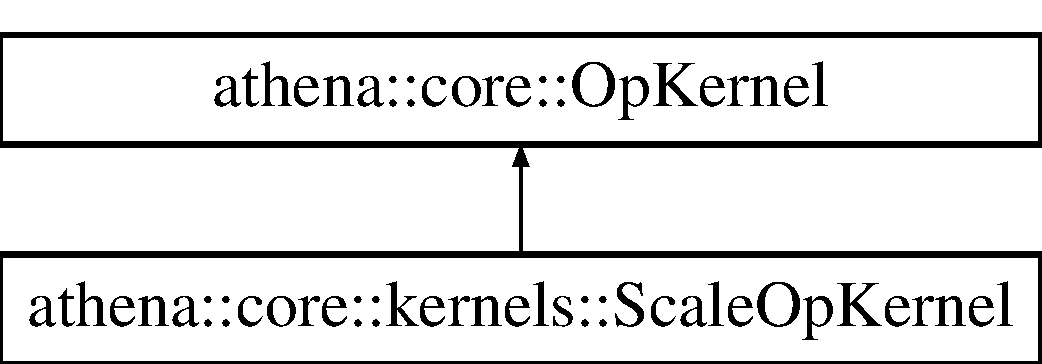
\includegraphics[height=2.000000cm]{classathena_1_1core_1_1kernels_1_1_scale_op_kernel}
\end{center}
\end{figure}
\subsection*{Public Member Functions}
\begin{DoxyCompactItemize}
\item 
int \mbox{\hyperlink{classathena_1_1core_1_1kernels_1_1_scale_op_kernel_a4f9e4fee100ed7f09840fa4b2d55f2bf}{get\+Operands\+Count}} () override
\item 
\mbox{\hyperlink{classathena_1_1core_1_1_tensor_shape}{athena\+::core\+::\+Tensor\+Shape}} \& \mbox{\hyperlink{classathena_1_1core_1_1kernels_1_1_scale_op_kernel_ad1791a60026e90c95f248202e1404a26}{get\+Output\+Shape}} (std\+::vector$<$ \mbox{\hyperlink{classathena_1_1core_1_1_tensor_shape}{athena\+::core\+::\+Tensor\+Shape}} $>$ \&shapes) override
\item 
\mbox{\hyperlink{classathena_1_1core_1_1_tensor_shape}{athena\+::core\+::\+Tensor\+Shape}} \& \mbox{\hyperlink{classathena_1_1core_1_1kernels_1_1_scale_op_kernel_ad7c63973c62e28c0ad3d854ce16debf1}{get\+Derivative\+Shape}} (int d, std\+::vector$<$ \mbox{\hyperlink{classathena_1_1core_1_1_tensor_shape}{athena\+::core\+::\+Tensor\+Shape}} $>$ \&shapes) override
\item 
\mbox{\Hypertarget{classathena_1_1core_1_1kernels_1_1_scale_op_kernel_a1b088e9abe5556913123a7c9c8880ec0}\label{classathena_1_1core_1_1kernels_1_1_scale_op_kernel_a1b088e9abe5556913123a7c9c8880ec0}} 
std\+::vector$<$ vm\+\_\+word $>$ {\bfseries get\+Op\+Bytecode} (std\+::vector$<$ vm\+\_\+word $>$ args, vm\+\_\+word result\+Cell) override
\item 
std\+::vector$<$ vm\+\_\+word $>$ \mbox{\hyperlink{classathena_1_1core_1_1kernels_1_1_scale_op_kernel_ad35869239968db73049161acbad05aab}{get\+Derivative\+Bytecode}} (int d, std\+::vector$<$ vm\+\_\+word $>$ args, vm\+\_\+word result\+Cell) override
\end{DoxyCompactItemize}
\subsection*{Additional Inherited Members}


\subsection{Detailed Description}
Multiply \mbox{\hyperlink{classathena_1_1core_1_1_tensor}{Tensor}} by scalar 

\subsection{Member Function Documentation}
\mbox{\Hypertarget{classathena_1_1core_1_1kernels_1_1_scale_op_kernel_ad35869239968db73049161acbad05aab}\label{classathena_1_1core_1_1kernels_1_1_scale_op_kernel_ad35869239968db73049161acbad05aab}} 
\index{athena\+::core\+::kernels\+::\+Scale\+Op\+Kernel@{athena\+::core\+::kernels\+::\+Scale\+Op\+Kernel}!get\+Derivative\+Bytecode@{get\+Derivative\+Bytecode}}
\index{get\+Derivative\+Bytecode@{get\+Derivative\+Bytecode}!athena\+::core\+::kernels\+::\+Scale\+Op\+Kernel@{athena\+::core\+::kernels\+::\+Scale\+Op\+Kernel}}
\subsubsection{\texorpdfstring{get\+Derivative\+Bytecode()}{getDerivativeBytecode()}}
{\footnotesize\ttfamily std\+::vector$<$ vm\+\_\+word $>$ athena\+::core\+::kernels\+::\+Scale\+Op\+Kernel\+::get\+Derivative\+Bytecode (\begin{DoxyParamCaption}\item[{int}]{d,  }\item[{std\+::vector$<$ vm\+\_\+word $>$}]{args,  }\item[{vm\+\_\+word}]{result\+Cell }\end{DoxyParamCaption})\hspace{0.3cm}{\ttfamily [override]}, {\ttfamily [virtual]}}

Generates bytecode to calculate partial derivative 
\begin{DoxyParams}{Parameters}
{\em d} & Number of variable with respect to which derivative is calculated \\
\hline
{\em args} & Function arguments \\
\hline
{\em result\+Cell} & Number of memory cell where results are saved \\
\hline
\end{DoxyParams}
\begin{DoxyReturn}{Returns}

\end{DoxyReturn}


Implements \mbox{\hyperlink{classathena_1_1core_1_1_op_kernel_ad500db1afc5a7c10acff8ecb8f1bee4d}{athena\+::core\+::\+Op\+Kernel}}.

\mbox{\Hypertarget{classathena_1_1core_1_1kernels_1_1_scale_op_kernel_ad7c63973c62e28c0ad3d854ce16debf1}\label{classathena_1_1core_1_1kernels_1_1_scale_op_kernel_ad7c63973c62e28c0ad3d854ce16debf1}} 
\index{athena\+::core\+::kernels\+::\+Scale\+Op\+Kernel@{athena\+::core\+::kernels\+::\+Scale\+Op\+Kernel}!get\+Derivative\+Shape@{get\+Derivative\+Shape}}
\index{get\+Derivative\+Shape@{get\+Derivative\+Shape}!athena\+::core\+::kernels\+::\+Scale\+Op\+Kernel@{athena\+::core\+::kernels\+::\+Scale\+Op\+Kernel}}
\subsubsection{\texorpdfstring{get\+Derivative\+Shape()}{getDerivativeShape()}}
{\footnotesize\ttfamily \mbox{\hyperlink{classathena_1_1core_1_1_tensor_shape}{athena\+::core\+::\+Tensor\+Shape}} \& athena\+::core\+::kernels\+::\+Scale\+Op\+Kernel\+::get\+Derivative\+Shape (\begin{DoxyParamCaption}\item[{int}]{d,  }\item[{std\+::vector$<$ \mbox{\hyperlink{classathena_1_1core_1_1_tensor_shape}{athena\+::core\+::\+Tensor\+Shape}} $>$ \&}]{shapes }\end{DoxyParamCaption})\hspace{0.3cm}{\ttfamily [override]}, {\ttfamily [virtual]}}

It is important for some operations to have certain size of their operands 
\begin{DoxyParams}{Parameters}
{\em shape} & Original operand shape \\
\hline
{\em dim} & Dimensionality \\
\hline
\end{DoxyParams}
\begin{DoxyReturn}{Returns}
New shape 
\end{DoxyReturn}


Implements \mbox{\hyperlink{classathena_1_1core_1_1_op_kernel_ad95af6dd184ce7ee9182ec7ca54b6c4d}{athena\+::core\+::\+Op\+Kernel}}.

\mbox{\Hypertarget{classathena_1_1core_1_1kernels_1_1_scale_op_kernel_a4f9e4fee100ed7f09840fa4b2d55f2bf}\label{classathena_1_1core_1_1kernels_1_1_scale_op_kernel_a4f9e4fee100ed7f09840fa4b2d55f2bf}} 
\index{athena\+::core\+::kernels\+::\+Scale\+Op\+Kernel@{athena\+::core\+::kernels\+::\+Scale\+Op\+Kernel}!get\+Operands\+Count@{get\+Operands\+Count}}
\index{get\+Operands\+Count@{get\+Operands\+Count}!athena\+::core\+::kernels\+::\+Scale\+Op\+Kernel@{athena\+::core\+::kernels\+::\+Scale\+Op\+Kernel}}
\subsubsection{\texorpdfstring{get\+Operands\+Count()}{getOperandsCount()}}
{\footnotesize\ttfamily int athena\+::core\+::kernels\+::\+Scale\+Op\+Kernel\+::get\+Operands\+Count (\begin{DoxyParamCaption}{ }\end{DoxyParamCaption})\hspace{0.3cm}{\ttfamily [override]}, {\ttfamily [virtual]}}

There can be unary, binary and other operations \begin{DoxyReturn}{Returns}
Number of operands accepted 
\end{DoxyReturn}


Implements \mbox{\hyperlink{classathena_1_1core_1_1_op_kernel_add97d4c132d80ecd9915acfedf7c9119}{athena\+::core\+::\+Op\+Kernel}}.

\mbox{\Hypertarget{classathena_1_1core_1_1kernels_1_1_scale_op_kernel_ad1791a60026e90c95f248202e1404a26}\label{classathena_1_1core_1_1kernels_1_1_scale_op_kernel_ad1791a60026e90c95f248202e1404a26}} 
\index{athena\+::core\+::kernels\+::\+Scale\+Op\+Kernel@{athena\+::core\+::kernels\+::\+Scale\+Op\+Kernel}!get\+Output\+Shape@{get\+Output\+Shape}}
\index{get\+Output\+Shape@{get\+Output\+Shape}!athena\+::core\+::kernels\+::\+Scale\+Op\+Kernel@{athena\+::core\+::kernels\+::\+Scale\+Op\+Kernel}}
\subsubsection{\texorpdfstring{get\+Output\+Shape()}{getOutputShape()}}
{\footnotesize\ttfamily \mbox{\hyperlink{classathena_1_1core_1_1_tensor_shape}{athena\+::core\+::\+Tensor\+Shape}} \& athena\+::core\+::kernels\+::\+Scale\+Op\+Kernel\+::get\+Output\+Shape (\begin{DoxyParamCaption}\item[{std\+::vector$<$ \mbox{\hyperlink{classathena_1_1core_1_1_tensor_shape}{athena\+::core\+::\+Tensor\+Shape}} $>$ \&}]{shapes }\end{DoxyParamCaption})\hspace{0.3cm}{\ttfamily [override]}, {\ttfamily [virtual]}}

It is important for some operations to have certain size of their operands 
\begin{DoxyParams}{Parameters}
{\em shape} & Original operand shape \\
\hline
{\em dim} & Dimensionality \\
\hline
\end{DoxyParams}
\begin{DoxyReturn}{Returns}
New shape 
\end{DoxyReturn}


Implements \mbox{\hyperlink{classathena_1_1core_1_1_op_kernel_a762e541463ffd089b47a8e6755c30fe1}{athena\+::core\+::\+Op\+Kernel}}.



The documentation for this class was generated from the following files\+:\begin{DoxyCompactItemize}
\item 
core/kernels/Scale\+Op\+Kernel.\+h\item 
core/kernels/Scale\+Op\+Kernel.\+cpp\end{DoxyCompactItemize}

\hypertarget{classathena_1_1core_1_1_session}{}\section{athena\+:\+:core\+:\+:Session Class Reference}
\label{classathena_1_1core_1_1_session}\index{athena\+::core\+::\+Session@{athena\+::core\+::\+Session}}


{\ttfamily \#include $<$Session.\+h$>$}

\subsection*{Public Member Functions}
\begin{DoxyCompactItemize}
\item 
void \mbox{\hyperlink{classathena_1_1core_1_1_session_a28b51416420aca2c39d9cf7ee81fe41d}{prepare}} (\mbox{\hyperlink{classathena_1_1core_1_1_node}{Node}} $\ast$logits)
\item 
\mbox{\hyperlink{classathena_1_1core_1_1_tensor}{Tensor}} $\ast$ \mbox{\hyperlink{classathena_1_1core_1_1_session_ab08af50ae0bbd2ed5171e1f45a7680ff}{run}} ()
\item 
\mbox{\Hypertarget{classathena_1_1core_1_1_session_a560fda7749519c69a5cafd889fd4077c}\label{classathena_1_1core_1_1_session_a560fda7749519c69a5cafd889fd4077c}} 
unsigned long {\bfseries get\+Result\+Cell} ()
\item 
\mbox{\Hypertarget{classathena_1_1core_1_1_session_a8aaab4641be2fe06e2ae098c366375e8}\label{classathena_1_1core_1_1_session_a8aaab4641be2fe06e2ae098c366375e8}} 
void {\bfseries set\+Executor} (\mbox{\hyperlink{classathena_1_1backend_1_1_abstract_executor}{athena\+::backend\+::\+Abstract\+Executor}} $\ast$exec)
\item 
\mbox{\Hypertarget{classathena_1_1core_1_1_session_a68b5280e3ce27634acbd0590ed0324ff}\label{classathena_1_1core_1_1_session_a68b5280e3ce27634acbd0590ed0324ff}} 
\mbox{\hyperlink{classathena_1_1backend_1_1_abstract_executor}{athena\+::backend\+::\+Abstract\+Executor}} $\ast$ {\bfseries get\+Executor} ()
\item 
\mbox{\Hypertarget{classathena_1_1core_1_1_session_ac9d7ec883d597138673716998180d905}\label{classathena_1_1core_1_1_session_ac9d7ec883d597138673716998180d905}} 
\mbox{\hyperlink{classathena_1_1backend_1_1_virtual_memory}{athena\+::backend\+::\+Virtual\+Memory}} $\ast$ {\bfseries get\+Memory} ()
\end{DoxyCompactItemize}


\subsection{Detailed Description}
The class encapsulates everything needed for a single training step 

Definition at line 28 of file Session.\+h.



\subsection{Member Function Documentation}
\mbox{\Hypertarget{classathena_1_1core_1_1_session_a28b51416420aca2c39d9cf7ee81fe41d}\label{classathena_1_1core_1_1_session_a28b51416420aca2c39d9cf7ee81fe41d}} 
\index{athena\+::core\+::\+Session@{athena\+::core\+::\+Session}!prepare@{prepare}}
\index{prepare@{prepare}!athena\+::core\+::\+Session@{athena\+::core\+::\+Session}}
\subsubsection{\texorpdfstring{prepare()}{prepare()}}
{\footnotesize\ttfamily void athena\+::core\+::\+Session\+::prepare (\begin{DoxyParamCaption}\item[{\mbox{\hyperlink{classathena_1_1core_1_1_node}{Node}} $\ast$}]{logits }\end{DoxyParamCaption})}

Generates bytecode for the whole graph 
\begin{DoxyParams}{Parameters}
{\em logits} & \\
\hline
\end{DoxyParams}


Definition at line 18 of file Session.\+cpp.

\mbox{\Hypertarget{classathena_1_1core_1_1_session_ab08af50ae0bbd2ed5171e1f45a7680ff}\label{classathena_1_1core_1_1_session_ab08af50ae0bbd2ed5171e1f45a7680ff}} 
\index{athena\+::core\+::\+Session@{athena\+::core\+::\+Session}!run@{run}}
\index{run@{run}!athena\+::core\+::\+Session@{athena\+::core\+::\+Session}}
\subsubsection{\texorpdfstring{run()}{run()}}
{\footnotesize\ttfamily \mbox{\hyperlink{classathena_1_1core_1_1_tensor}{athena\+::core\+::\+Tensor}} $\ast$ athena\+::core\+::\+Session\+::run (\begin{DoxyParamCaption}{ }\end{DoxyParamCaption})}

does single training step \begin{DoxyReturn}{Returns}
result tensor 
\end{DoxyReturn}


Definition at line 126 of file Session.\+cpp.



The documentation for this class was generated from the following files\+:\begin{DoxyCompactItemize}
\item 
core/Session.\+h\item 
core/Session.\+cpp\end{DoxyCompactItemize}

\hypertarget{classathena_1_1core_1_1optimizers_1_1_s_g_d_optimizer}{}\section{athena\+:\+:core\+:\+:optimizers\+:\+:S\+G\+D\+Optimizer Class Reference}
\label{classathena_1_1core_1_1optimizers_1_1_s_g_d_optimizer}\index{athena\+::core\+::optimizers\+::\+S\+G\+D\+Optimizer@{athena\+::core\+::optimizers\+::\+S\+G\+D\+Optimizer}}
Inheritance diagram for athena\+:\+:core\+:\+:optimizers\+:\+:S\+G\+D\+Optimizer\+:\begin{figure}[H]
\begin{center}
\leavevmode
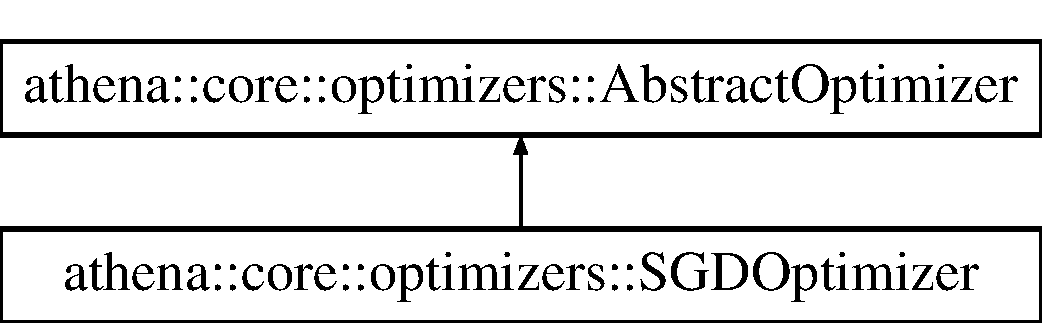
\includegraphics[height=2.000000cm]{d2/db8/classathena_1_1core_1_1optimizers_1_1_s_g_d_optimizer}
\end{center}
\end{figure}
\subsection*{Public Member Functions}
\begin{DoxyCompactItemize}
\item 
\mbox{\Hypertarget{classathena_1_1core_1_1optimizers_1_1_s_g_d_optimizer_a7b49822dc95f2e603d1f96b9a3ea529c}\label{classathena_1_1core_1_1optimizers_1_1_s_g_d_optimizer_a7b49822dc95f2e603d1f96b9a3ea529c}} 
{\bfseries S\+G\+D\+Optimizer} (\mbox{\hyperlink{classathena_1_1core_1_1loss_1_1_abstract_loss_function}{athena\+::core\+::loss\+::\+Abstract\+Loss\+Function}} $\ast$logits)
\end{DoxyCompactItemize}
\subsection*{Additional Inherited Members}


\subsection{Detailed Description}


Definition at line 13 of file S\+G\+D\+Optimizer.\+h.



The documentation for this class was generated from the following file\+:\begin{DoxyCompactItemize}
\item 
core/optimizers/S\+G\+D\+Optimizer.\+h\end{DoxyCompactItemize}

\hypertarget{classathena_1_1core_1_1kernels_1_1_sigmoid_op_kernel}{}\section{athena\+:\+:core\+:\+:kernels\+:\+:Sigmoid\+Op\+Kernel Class Reference}
\label{classathena_1_1core_1_1kernels_1_1_sigmoid_op_kernel}\index{athena\+::core\+::kernels\+::\+Sigmoid\+Op\+Kernel@{athena\+::core\+::kernels\+::\+Sigmoid\+Op\+Kernel}}


{\ttfamily \#include $<$Sigmoid\+Op\+Kernel.\+h$>$}

Inheritance diagram for athena\+:\+:core\+:\+:kernels\+:\+:Sigmoid\+Op\+Kernel\+:\begin{figure}[H]
\begin{center}
\leavevmode
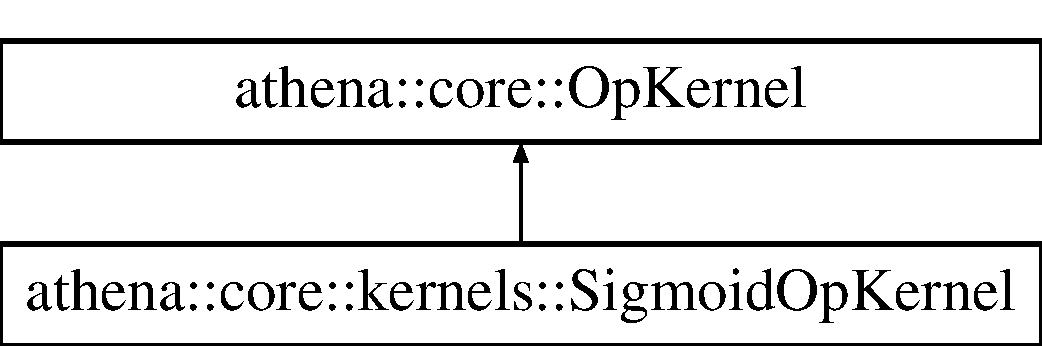
\includegraphics[height=2.000000cm]{d0/dac/classathena_1_1core_1_1kernels_1_1_sigmoid_op_kernel}
\end{center}
\end{figure}
\subsection*{Public Member Functions}
\begin{DoxyCompactItemize}
\item 
int \mbox{\hyperlink{classathena_1_1core_1_1kernels_1_1_sigmoid_op_kernel_acb639510462e759a92747cec8c32358b}{get\+Operands\+Count}} () override
\item 
\mbox{\hyperlink{classathena_1_1core_1_1_tensor_shape}{athena\+::core\+::\+Tensor\+Shape}} \& \mbox{\hyperlink{classathena_1_1core_1_1kernels_1_1_sigmoid_op_kernel_abd929f41de55a4898a0fce70025c1499}{get\+Output\+Shape}} (std\+::vector$<$ \mbox{\hyperlink{classathena_1_1core_1_1_tensor_shape}{athena\+::core\+::\+Tensor\+Shape}} $>$ \&shapes) override
\item 
\mbox{\hyperlink{classathena_1_1core_1_1_tensor_shape}{athena\+::core\+::\+Tensor\+Shape}} \& \mbox{\hyperlink{classathena_1_1core_1_1kernels_1_1_sigmoid_op_kernel_a0ea18b43eb9355d7a855202898ff09fc}{get\+Derivative\+Shape}} (int d, std\+::vector$<$ \mbox{\hyperlink{classathena_1_1core_1_1_tensor_shape}{athena\+::core\+::\+Tensor\+Shape}} $>$ \&shapes) override
\item 
\mbox{\Hypertarget{classathena_1_1core_1_1kernels_1_1_sigmoid_op_kernel_a728bbcf1fce2ae1173f45119ae0898fc}\label{classathena_1_1core_1_1kernels_1_1_sigmoid_op_kernel_a728bbcf1fce2ae1173f45119ae0898fc}} 
std\+::vector$<$ vm\+\_\+word $>$ {\bfseries get\+Op\+Bytecode} (std\+::vector$<$ vm\+\_\+word $>$ args, vm\+\_\+word result\+Cell) override
\item 
std\+::vector$<$ vm\+\_\+word $>$ \mbox{\hyperlink{classathena_1_1core_1_1kernels_1_1_sigmoid_op_kernel_a38166ae2204692353efa2f6270714a80}{get\+Derivative\+Bytecode}} (int d, std\+::vector$<$ vm\+\_\+word $>$ args, vm\+\_\+word result\+Cell) override
\end{DoxyCompactItemize}
\subsection*{Additional Inherited Members}


\subsection{Detailed Description}
Apply sigmoid function to every element of \mbox{\hyperlink{classathena_1_1core_1_1_tensor}{Tensor}}. See \href{https://en.wikipedia.org/wiki/Sigmoid_function}{\tt https\+://en.\+wikipedia.\+org/wiki/\+Sigmoid\+\_\+function} for more info 

Definition at line 17 of file Sigmoid\+Op\+Kernel.\+h.



\subsection{Member Function Documentation}
\mbox{\Hypertarget{classathena_1_1core_1_1kernels_1_1_sigmoid_op_kernel_a38166ae2204692353efa2f6270714a80}\label{classathena_1_1core_1_1kernels_1_1_sigmoid_op_kernel_a38166ae2204692353efa2f6270714a80}} 
\index{athena\+::core\+::kernels\+::\+Sigmoid\+Op\+Kernel@{athena\+::core\+::kernels\+::\+Sigmoid\+Op\+Kernel}!get\+Derivative\+Bytecode@{get\+Derivative\+Bytecode}}
\index{get\+Derivative\+Bytecode@{get\+Derivative\+Bytecode}!athena\+::core\+::kernels\+::\+Sigmoid\+Op\+Kernel@{athena\+::core\+::kernels\+::\+Sigmoid\+Op\+Kernel}}
\subsubsection{\texorpdfstring{get\+Derivative\+Bytecode()}{getDerivativeBytecode()}}
{\footnotesize\ttfamily std\+::vector$<$ vm\+\_\+word $>$ athena\+::core\+::kernels\+::\+Sigmoid\+Op\+Kernel\+::get\+Derivative\+Bytecode (\begin{DoxyParamCaption}\item[{int}]{d,  }\item[{std\+::vector$<$ vm\+\_\+word $>$}]{args,  }\item[{vm\+\_\+word}]{result\+Cell }\end{DoxyParamCaption})\hspace{0.3cm}{\ttfamily [override]}, {\ttfamily [virtual]}}

Generates bytecode to calculate partial derivative 
\begin{DoxyParams}{Parameters}
{\em d} & Number of variable with respect to which derivative is calculated \\
\hline
{\em args} & Function arguments \\
\hline
{\em result\+Cell} & Number of memory cell where results are saved \\
\hline
\end{DoxyParams}
\begin{DoxyReturn}{Returns}

\end{DoxyReturn}


Implements \mbox{\hyperlink{classathena_1_1core_1_1_op_kernel_ad500db1afc5a7c10acff8ecb8f1bee4d}{athena\+::core\+::\+Op\+Kernel}}.



Definition at line 29 of file Sigmoid\+Op\+Kernel.\+cpp.

\mbox{\Hypertarget{classathena_1_1core_1_1kernels_1_1_sigmoid_op_kernel_a0ea18b43eb9355d7a855202898ff09fc}\label{classathena_1_1core_1_1kernels_1_1_sigmoid_op_kernel_a0ea18b43eb9355d7a855202898ff09fc}} 
\index{athena\+::core\+::kernels\+::\+Sigmoid\+Op\+Kernel@{athena\+::core\+::kernels\+::\+Sigmoid\+Op\+Kernel}!get\+Derivative\+Shape@{get\+Derivative\+Shape}}
\index{get\+Derivative\+Shape@{get\+Derivative\+Shape}!athena\+::core\+::kernels\+::\+Sigmoid\+Op\+Kernel@{athena\+::core\+::kernels\+::\+Sigmoid\+Op\+Kernel}}
\subsubsection{\texorpdfstring{get\+Derivative\+Shape()}{getDerivativeShape()}}
{\footnotesize\ttfamily \mbox{\hyperlink{classathena_1_1core_1_1_tensor_shape}{athena\+::core\+::\+Tensor\+Shape}} \& athena\+::core\+::kernels\+::\+Sigmoid\+Op\+Kernel\+::get\+Derivative\+Shape (\begin{DoxyParamCaption}\item[{int}]{d,  }\item[{std\+::vector$<$ \mbox{\hyperlink{classathena_1_1core_1_1_tensor_shape}{athena\+::core\+::\+Tensor\+Shape}} $>$ \&}]{shapes }\end{DoxyParamCaption})\hspace{0.3cm}{\ttfamily [override]}, {\ttfamily [virtual]}}

It is important for some operations to have certain size of their operands 
\begin{DoxyParams}{Parameters}
{\em shape} & Original operand shape \\
\hline
{\em dim} & Dimensionality \\
\hline
\end{DoxyParams}
\begin{DoxyReturn}{Returns}
New shape 
\end{DoxyReturn}


Implements \mbox{\hyperlink{classathena_1_1core_1_1_op_kernel_ad95af6dd184ce7ee9182ec7ca54b6c4d}{athena\+::core\+::\+Op\+Kernel}}.



Definition at line 44 of file Sigmoid\+Op\+Kernel.\+cpp.

\mbox{\Hypertarget{classathena_1_1core_1_1kernels_1_1_sigmoid_op_kernel_acb639510462e759a92747cec8c32358b}\label{classathena_1_1core_1_1kernels_1_1_sigmoid_op_kernel_acb639510462e759a92747cec8c32358b}} 
\index{athena\+::core\+::kernels\+::\+Sigmoid\+Op\+Kernel@{athena\+::core\+::kernels\+::\+Sigmoid\+Op\+Kernel}!get\+Operands\+Count@{get\+Operands\+Count}}
\index{get\+Operands\+Count@{get\+Operands\+Count}!athena\+::core\+::kernels\+::\+Sigmoid\+Op\+Kernel@{athena\+::core\+::kernels\+::\+Sigmoid\+Op\+Kernel}}
\subsubsection{\texorpdfstring{get\+Operands\+Count()}{getOperandsCount()}}
{\footnotesize\ttfamily int athena\+::core\+::kernels\+::\+Sigmoid\+Op\+Kernel\+::get\+Operands\+Count (\begin{DoxyParamCaption}{ }\end{DoxyParamCaption})\hspace{0.3cm}{\ttfamily [override]}, {\ttfamily [virtual]}}

There can be unary, binary and other operations \begin{DoxyReturn}{Returns}
Number of operands accepted 
\end{DoxyReturn}


Implements \mbox{\hyperlink{classathena_1_1core_1_1_op_kernel_add97d4c132d80ecd9915acfedf7c9119}{athena\+::core\+::\+Op\+Kernel}}.



Definition at line 10 of file Sigmoid\+Op\+Kernel.\+cpp.

\mbox{\Hypertarget{classathena_1_1core_1_1kernels_1_1_sigmoid_op_kernel_abd929f41de55a4898a0fce70025c1499}\label{classathena_1_1core_1_1kernels_1_1_sigmoid_op_kernel_abd929f41de55a4898a0fce70025c1499}} 
\index{athena\+::core\+::kernels\+::\+Sigmoid\+Op\+Kernel@{athena\+::core\+::kernels\+::\+Sigmoid\+Op\+Kernel}!get\+Output\+Shape@{get\+Output\+Shape}}
\index{get\+Output\+Shape@{get\+Output\+Shape}!athena\+::core\+::kernels\+::\+Sigmoid\+Op\+Kernel@{athena\+::core\+::kernels\+::\+Sigmoid\+Op\+Kernel}}
\subsubsection{\texorpdfstring{get\+Output\+Shape()}{getOutputShape()}}
{\footnotesize\ttfamily \mbox{\hyperlink{classathena_1_1core_1_1_tensor_shape}{athena\+::core\+::\+Tensor\+Shape}} \& athena\+::core\+::kernels\+::\+Sigmoid\+Op\+Kernel\+::get\+Output\+Shape (\begin{DoxyParamCaption}\item[{std\+::vector$<$ \mbox{\hyperlink{classathena_1_1core_1_1_tensor_shape}{athena\+::core\+::\+Tensor\+Shape}} $>$ \&}]{shapes }\end{DoxyParamCaption})\hspace{0.3cm}{\ttfamily [override]}, {\ttfamily [virtual]}}

It is important for some operations to have certain size of their operands 
\begin{DoxyParams}{Parameters}
{\em shape} & Original operand shape \\
\hline
{\em dim} & Dimensionality \\
\hline
\end{DoxyParams}
\begin{DoxyReturn}{Returns}
New shape 
\end{DoxyReturn}


Implements \mbox{\hyperlink{classathena_1_1core_1_1_op_kernel_a762e541463ffd089b47a8e6755c30fe1}{athena\+::core\+::\+Op\+Kernel}}.



Definition at line 50 of file Sigmoid\+Op\+Kernel.\+cpp.



The documentation for this class was generated from the following files\+:\begin{DoxyCompactItemize}
\item 
core/kernels/Sigmoid\+Op\+Kernel.\+h\item 
core/kernels/Sigmoid\+Op\+Kernel.\+cpp\end{DoxyCompactItemize}

\hypertarget{structathena_1_1backend_1_1generic_1_1_swap_record}{}\section{athena\+:\+:backend\+:\+:generic\+:\+:Swap\+Record Struct Reference}
\label{structathena_1_1backend_1_1generic_1_1_swap_record}\index{athena\+::backend\+::generic\+::\+Swap\+Record@{athena\+::backend\+::generic\+::\+Swap\+Record}}


{\ttfamily \#include $<$Generic\+Memory\+Manager.\+h$>$}

\subsection*{Public Attributes}
\begin{DoxyCompactItemize}
\item 
\mbox{\Hypertarget{structathena_1_1backend_1_1generic_1_1_swap_record_ac3ffe37973d1992220844a94c8b6afcb}\label{structathena_1_1backend_1_1generic_1_1_swap_record_ac3ffe37973d1992220844a94c8b6afcb}} 
vm\+\_\+word {\bfseries address}
\item 
\mbox{\Hypertarget{structathena_1_1backend_1_1generic_1_1_swap_record_ad4851011bc4d109f47c5610e817978de}\label{structathena_1_1backend_1_1generic_1_1_swap_record_ad4851011bc4d109f47c5610e817978de}} 
size\+\_\+t {\bfseries length}
\item 
\mbox{\Hypertarget{structathena_1_1backend_1_1generic_1_1_swap_record_ae3f76aea814f0e9b0d6fabbfa349c54a}\label{structathena_1_1backend_1_1generic_1_1_swap_record_ae3f76aea814f0e9b0d6fabbfa349c54a}} 
std\+::string {\bfseries filename}
\end{DoxyCompactItemize}


\subsection{Detailed Description}
Describes single swap record -\/ a file, that stores Tensor data 

Definition at line 21 of file Generic\+Memory\+Manager.\+h.



The documentation for this struct was generated from the following file\+:\begin{DoxyCompactItemize}
\item 
backend/generic/Generic\+Memory\+Manager.\+h\end{DoxyCompactItemize}

\hypertarget{classathena_1_1core_1_1_tensor}{}\section{athena\+:\+:core\+:\+:Tensor Class Reference}
\label{classathena_1_1core_1_1_tensor}\index{athena\+::core\+::\+Tensor@{athena\+::core\+::\+Tensor}}


{\ttfamily \#include $<$Tensor.\+h$>$}

\subsection*{Public Member Functions}
\begin{DoxyCompactItemize}
\item 
\mbox{\Hypertarget{classathena_1_1core_1_1_tensor_a73df0da6b63c55ef90c4941aa23acc54}\label{classathena_1_1core_1_1_tensor_a73df0da6b63c55ef90c4941aa23acc54}} 
{\bfseries Tensor} (const \mbox{\hyperlink{classathena_1_1core_1_1_tensor_shape}{Tensor\+Shape}} \&shape, Data\+Type data\+Type)
\item 
\mbox{\Hypertarget{classathena_1_1core_1_1_tensor_af07b079821aadb1ec80c98b14617f2cb}\label{classathena_1_1core_1_1_tensor_af07b079821aadb1ec80c98b14617f2cb}} 
const \mbox{\hyperlink{classathena_1_1core_1_1_tensor_shape}{Tensor\+Shape}} \& {\bfseries get\+Shape} () const
\item 
\mbox{\Hypertarget{classathena_1_1core_1_1_tensor_ac808b57b581b28ef78244bdc1f7eba0e}\label{classathena_1_1core_1_1_tensor_ac808b57b581b28ef78244bdc1f7eba0e}} 
Data\+Type {\bfseries get\+Type} () const
\item 
\mbox{\Hypertarget{classathena_1_1core_1_1_tensor_ae864cbc773fa869a90bce479f03dbf68}\label{classathena_1_1core_1_1_tensor_ae864cbc773fa869a90bce479f03dbf68}} 
vm\+\_\+word {\bfseries get\+Start\+Address} ()
\item 
\mbox{\Hypertarget{classathena_1_1core_1_1_tensor_a863c18e892c319b1e7fd359ddc7282ca}\label{classathena_1_1core_1_1_tensor_a863c18e892c319b1e7fd359ddc7282ca}} 
void {\bfseries set\+Start\+Address} (vm\+\_\+word address)
\item 
\mbox{\Hypertarget{classathena_1_1core_1_1_tensor_a98c05789432a4201a92ed2f7221d6882}\label{classathena_1_1core_1_1_tensor_a98c05789432a4201a92ed2f7221d6882}} 
\mbox{\hyperlink{classathena_1_1core_1_1_tensor}{Tensor}} \& {\bfseries operator\mbox{[}$\,$\mbox{]}} (unsigned int idx)
\end{DoxyCompactItemize}


\subsection{Detailed Description}
In mathematics {\bfseries tensor} is an abstract object, expressing some definite type of multi-\/linear concept. See \href{https://en.wikipedia.org/wiki/Tensor_(intrinsic_definition)}{\tt Wikipedia} for more info. 

In Athena \mbox{\hyperlink{classathena_1_1core_1_1_tensor}{Tensor}} is an abstraction to represent data inside computational graph. A 1-\/dimensional \mbox{\hyperlink{classathena_1_1core_1_1_tensor}{Tensor}} is either scalar or vector. A 2-\/dimensional \mbox{\hyperlink{classathena_1_1core_1_1_tensor}{Tensor}} is a matrix. 

Definition at line 29 of file Tensor.\+h.



The documentation for this class was generated from the following files\+:\begin{DoxyCompactItemize}
\item 
core/Tensor.\+h\item 
core/Tensor.\+cpp\end{DoxyCompactItemize}

\hypertarget{classathena_1_1core_1_1_tensor_shape}{}\section{athena\+:\+:core\+:\+:Tensor\+Shape Class Reference}
\label{classathena_1_1core_1_1_tensor_shape}\index{athena\+::core\+::\+Tensor\+Shape@{athena\+::core\+::\+Tensor\+Shape}}


{\ttfamily \#include $<$Tensor\+Shape.\+h$>$}

\subsection*{Public Member Functions}
\begin{DoxyCompactItemize}
\item 
\mbox{\Hypertarget{classathena_1_1core_1_1_tensor_shape_ad20d31bd783690b3297831f0269e88a7}\label{classathena_1_1core_1_1_tensor_shape_ad20d31bd783690b3297831f0269e88a7}} 
{\bfseries Tensor\+Shape} (std\+::vector$<$ size\+\_\+t $>$ shape)
\item 
\mbox{\Hypertarget{classathena_1_1core_1_1_tensor_shape_afee84a39eb172f5285dbef6fd1e730e2}\label{classathena_1_1core_1_1_tensor_shape_afee84a39eb172f5285dbef6fd1e730e2}} 
{\bfseries Tensor\+Shape} (unsigned long $\ast$shape, unsigned long length)
\item 
\mbox{\Hypertarget{classathena_1_1core_1_1_tensor_shape_a4e64dcd3893bf156602edab7112ccf4e}\label{classathena_1_1core_1_1_tensor_shape_a4e64dcd3893bf156602edab7112ccf4e}} 
{\bfseries Tensor\+Shape} (const \mbox{\hyperlink{classathena_1_1core_1_1_tensor_shape}{Tensor\+Shape}} \&)
\item 
\mbox{\Hypertarget{classathena_1_1core_1_1_tensor_shape_a75503b33e07596367c175d7667d354f5}\label{classathena_1_1core_1_1_tensor_shape_a75503b33e07596367c175d7667d354f5}} 
\mbox{\hyperlink{classathena_1_1core_1_1_tensor_shape}{Tensor\+Shape}} \& {\bfseries operator=} (const \mbox{\hyperlink{classathena_1_1core_1_1_tensor_shape}{Tensor\+Shape}} \&)
\item 
unsigned long \mbox{\hyperlink{classathena_1_1core_1_1_tensor_shape_a73f686650f41bd7fa065aa16dfc4529f}{dimensions}} () const
\item 
unsigned long \mbox{\hyperlink{classathena_1_1core_1_1_tensor_shape_ac0433f4e7a42e5307bb9fb976befdd47}{dim}} (unsigned long n) const
\item 
unsigned long \mbox{\hyperlink{classathena_1_1core_1_1_tensor_shape_a81219fb0b0e3e6852cb02fbbcf059882}{total\+Size}} () const
\item 
\mbox{\Hypertarget{classathena_1_1core_1_1_tensor_shape_ab76bd8f258b315eedcae3eae2d46a73d}\label{classathena_1_1core_1_1_tensor_shape_ab76bd8f258b315eedcae3eae2d46a73d}} 
const std\+::vector$<$ unsigned long $>$ \& {\bfseries get\+Shape} () const
\item 
bool \mbox{\hyperlink{classathena_1_1core_1_1_tensor_shape_aa42737e3e51e76507bb60791889d4d9b}{operator==}} (const \mbox{\hyperlink{classathena_1_1core_1_1_tensor_shape}{Tensor\+Shape}} \&) const
\item 
bool \mbox{\hyperlink{classathena_1_1core_1_1_tensor_shape_acdb5b20f9922cb4d7ee29a868fd05b1b}{operator!=}} (const \mbox{\hyperlink{classathena_1_1core_1_1_tensor_shape}{Tensor\+Shape}} \&rhs) const
\end{DoxyCompactItemize}


\subsection{Detailed Description}
Class represents size parameters for \mbox{\hyperlink{classathena_1_1core_1_1_tensor}{Tensor}} 

Definition at line 25 of file Tensor\+Shape.\+h.



\subsection{Member Function Documentation}
\mbox{\Hypertarget{classathena_1_1core_1_1_tensor_shape_ac0433f4e7a42e5307bb9fb976befdd47}\label{classathena_1_1core_1_1_tensor_shape_ac0433f4e7a42e5307bb9fb976befdd47}} 
\index{athena\+::core\+::\+Tensor\+Shape@{athena\+::core\+::\+Tensor\+Shape}!dim@{dim}}
\index{dim@{dim}!athena\+::core\+::\+Tensor\+Shape@{athena\+::core\+::\+Tensor\+Shape}}
\subsubsection{\texorpdfstring{dim()}{dim()}}
{\footnotesize\ttfamily unsigned long athena\+::core\+::\+Tensor\+Shape\+::dim (\begin{DoxyParamCaption}\item[{unsigned long}]{n }\end{DoxyParamCaption}) const}

Gives size for certain dimension 
\begin{DoxyParams}{Parameters}
{\em n} & Dimension index ( 0 $<$= d $<$ dimensions ) \\
\hline
\end{DoxyParams}
\begin{DoxyReturn}{Returns}
Size of dimension n 
\end{DoxyReturn}


Definition at line 33 of file Tensor\+Shape.\+cpp.



Referenced by operator==().

\mbox{\Hypertarget{classathena_1_1core_1_1_tensor_shape_a73f686650f41bd7fa065aa16dfc4529f}\label{classathena_1_1core_1_1_tensor_shape_a73f686650f41bd7fa065aa16dfc4529f}} 
\index{athena\+::core\+::\+Tensor\+Shape@{athena\+::core\+::\+Tensor\+Shape}!dimensions@{dimensions}}
\index{dimensions@{dimensions}!athena\+::core\+::\+Tensor\+Shape@{athena\+::core\+::\+Tensor\+Shape}}
\subsubsection{\texorpdfstring{dimensions()}{dimensions()}}
{\footnotesize\ttfamily unsigned long athena\+::core\+::\+Tensor\+Shape\+::dimensions (\begin{DoxyParamCaption}{ }\end{DoxyParamCaption}) const}

\begin{DoxyReturn}{Returns}
Number of dimensions in \mbox{\hyperlink{classathena_1_1core_1_1_tensor}{Tensor}} 
\end{DoxyReturn}


Definition at line 29 of file Tensor\+Shape.\+cpp.



Referenced by operator==().

\mbox{\Hypertarget{classathena_1_1core_1_1_tensor_shape_acdb5b20f9922cb4d7ee29a868fd05b1b}\label{classathena_1_1core_1_1_tensor_shape_acdb5b20f9922cb4d7ee29a868fd05b1b}} 
\index{athena\+::core\+::\+Tensor\+Shape@{athena\+::core\+::\+Tensor\+Shape}!operator"!=@{operator"!=}}
\index{operator"!=@{operator"!=}!athena\+::core\+::\+Tensor\+Shape@{athena\+::core\+::\+Tensor\+Shape}}
\subsubsection{\texorpdfstring{operator"!=()}{operator!=()}}
{\footnotesize\ttfamily bool athena\+::core\+::\+Tensor\+Shape\+::operator!= (\begin{DoxyParamCaption}\item[{const \mbox{\hyperlink{classathena_1_1core_1_1_tensor_shape}{Tensor\+Shape}} \&}]{rhs }\end{DoxyParamCaption}) const}


\begin{DoxyParams}{Parameters}
{\em rhs} & \mbox{\hyperlink{classathena_1_1core_1_1_tensor_shape}{Tensor\+Shape}} to be compared with \\
\hline
\end{DoxyParams}
\begin{DoxyReturn}{Returns}
True if dimensions are different, else False 
\end{DoxyReturn}


Definition at line 58 of file Tensor\+Shape.\+cpp.

\mbox{\Hypertarget{classathena_1_1core_1_1_tensor_shape_aa42737e3e51e76507bb60791889d4d9b}\label{classathena_1_1core_1_1_tensor_shape_aa42737e3e51e76507bb60791889d4d9b}} 
\index{athena\+::core\+::\+Tensor\+Shape@{athena\+::core\+::\+Tensor\+Shape}!operator==@{operator==}}
\index{operator==@{operator==}!athena\+::core\+::\+Tensor\+Shape@{athena\+::core\+::\+Tensor\+Shape}}
\subsubsection{\texorpdfstring{operator==()}{operator==()}}
{\footnotesize\ttfamily bool athena\+::core\+::\+Tensor\+Shape\+::operator== (\begin{DoxyParamCaption}\item[{const \mbox{\hyperlink{classathena_1_1core_1_1_tensor_shape}{Tensor\+Shape}} \&}]{rhs }\end{DoxyParamCaption}) const}

\begin{DoxyReturn}{Returns}
True if dimensions are equal, else False 
\end{DoxyReturn}


Definition at line 42 of file Tensor\+Shape.\+cpp.

\mbox{\Hypertarget{classathena_1_1core_1_1_tensor_shape_a81219fb0b0e3e6852cb02fbbcf059882}\label{classathena_1_1core_1_1_tensor_shape_a81219fb0b0e3e6852cb02fbbcf059882}} 
\index{athena\+::core\+::\+Tensor\+Shape@{athena\+::core\+::\+Tensor\+Shape}!total\+Size@{total\+Size}}
\index{total\+Size@{total\+Size}!athena\+::core\+::\+Tensor\+Shape@{athena\+::core\+::\+Tensor\+Shape}}
\subsubsection{\texorpdfstring{total\+Size()}{totalSize()}}
{\footnotesize\ttfamily unsigned long athena\+::core\+::\+Tensor\+Shape\+::total\+Size (\begin{DoxyParamCaption}{ }\end{DoxyParamCaption}) const}

\begin{DoxyReturn}{Returns}
Total number of elements in \mbox{\hyperlink{classathena_1_1core_1_1_tensor}{Tensor}} 
\end{DoxyReturn}


Definition at line 17 of file Tensor\+Shape.\+cpp.



Referenced by athena\+::backend\+::\+Virtual\+Memory\+::allocate(), athena\+::backend\+::\+Abstract\+Memory\+Manager\+::allocate\+And\+Lock(), and athena\+::backend\+::\+Abstract\+Memory\+Manager\+::load\+And\+Lock().



The documentation for this class was generated from the following files\+:\begin{DoxyCompactItemize}
\item 
core/Tensor\+Shape.\+h\item 
core/Tensor\+Shape.\+cpp\end{DoxyCompactItemize}

\hypertarget{classathena_1_1backend_1_1_virtual_memory}{}\section{athena\+:\+:backend\+:\+:Virtual\+Memory Class Reference}
\label{classathena_1_1backend_1_1_virtual_memory}\index{athena\+::backend\+::\+Virtual\+Memory@{athena\+::backend\+::\+Virtual\+Memory}}


{\ttfamily \#include $<$Virtual\+Memory.\+h$>$}

\subsection*{Public Member Functions}
\begin{DoxyCompactItemize}
\item 
vm\+\_\+word \mbox{\hyperlink{classathena_1_1backend_1_1_virtual_memory_a22be58a8e0cb574a7d46d4095cb64ac5}{allocate}} (\mbox{\hyperlink{classathena_1_1core_1_1_tensor}{athena\+::core\+::\+Tensor}} $\ast$tensor)
\item 
void \mbox{\hyperlink{classathena_1_1backend_1_1_virtual_memory_a73815358c436f8f6dd73d49d4d5d189d}{free}} (\mbox{\hyperlink{classathena_1_1core_1_1_tensor}{athena\+::core\+::\+Tensor}} $\ast$tensor)
\item 
void \mbox{\hyperlink{classathena_1_1backend_1_1_virtual_memory_ab24e17b8e8b2f8278b56b84dfdda42a3}{free}} (vm\+\_\+word virtual\+Address)
\end{DoxyCompactItemize}


\subsection{Detailed Description}
Virtual memory is an abstraction of storage resources that are actually available on a given machine. Each thread has its own address space. In Athena\textquotesingle{}s VM address space is linear. This means that valid addresses are 0 to 2$^\wedge$64 -\/ 1. Address 0 is reserved for N\+U\+LL value. When Tensor is initialized, it is given with a continuous block of virtual addresses. When one actually needs to access Tensor\textquotesingle{}s data, Memory Manager allocates physical memory and converts virtual addresses to physical ones. This helps Athena to run in low-\/memory conditions. This class is heavily used in Session class to generate bytecode. ~\newline
 To discover more about Virtual Memory see article on \href{https://en.wikipedia.org/wiki/Virtual_memory}{\tt Wikipedia} 

\subsection{Member Function Documentation}
\mbox{\Hypertarget{classathena_1_1backend_1_1_virtual_memory_a22be58a8e0cb574a7d46d4095cb64ac5}\label{classathena_1_1backend_1_1_virtual_memory_a22be58a8e0cb574a7d46d4095cb64ac5}} 
\index{athena\+::backend\+::\+Virtual\+Memory@{athena\+::backend\+::\+Virtual\+Memory}!allocate@{allocate}}
\index{allocate@{allocate}!athena\+::backend\+::\+Virtual\+Memory@{athena\+::backend\+::\+Virtual\+Memory}}
\subsubsection{\texorpdfstring{allocate()}{allocate()}}
{\footnotesize\ttfamily vm\+\_\+word athena\+::backend\+::\+Virtual\+Memory\+::allocate (\begin{DoxyParamCaption}\item[{\mbox{\hyperlink{classathena_1_1core_1_1_tensor}{athena\+::core\+::\+Tensor}} $\ast$}]{tensor }\end{DoxyParamCaption})}

Allocates virtual memory for given Tensor 
\begin{DoxyParams}{Parameters}
{\em tensor} & Tensor object \\
\hline
\end{DoxyParams}
\begin{DoxyReturn}{Returns}
Virtual Address of 0 element of Tensor 
\end{DoxyReturn}
\mbox{\Hypertarget{classathena_1_1backend_1_1_virtual_memory_a73815358c436f8f6dd73d49d4d5d189d}\label{classathena_1_1backend_1_1_virtual_memory_a73815358c436f8f6dd73d49d4d5d189d}} 
\index{athena\+::backend\+::\+Virtual\+Memory@{athena\+::backend\+::\+Virtual\+Memory}!free@{free}}
\index{free@{free}!athena\+::backend\+::\+Virtual\+Memory@{athena\+::backend\+::\+Virtual\+Memory}}
\subsubsection{\texorpdfstring{free()}{free()}\hspace{0.1cm}{\footnotesize\ttfamily [1/2]}}
{\footnotesize\ttfamily void athena\+::backend\+::\+Virtual\+Memory\+::free (\begin{DoxyParamCaption}\item[{\mbox{\hyperlink{classathena_1_1core_1_1_tensor}{athena\+::core\+::\+Tensor}} $\ast$}]{tensor }\end{DoxyParamCaption})}

Marks memory as free 
\begin{DoxyParams}{Parameters}
{\em tensor} & Corresponding tensor \\
\hline
\end{DoxyParams}
\mbox{\Hypertarget{classathena_1_1backend_1_1_virtual_memory_ab24e17b8e8b2f8278b56b84dfdda42a3}\label{classathena_1_1backend_1_1_virtual_memory_ab24e17b8e8b2f8278b56b84dfdda42a3}} 
\index{athena\+::backend\+::\+Virtual\+Memory@{athena\+::backend\+::\+Virtual\+Memory}!free@{free}}
\index{free@{free}!athena\+::backend\+::\+Virtual\+Memory@{athena\+::backend\+::\+Virtual\+Memory}}
\subsubsection{\texorpdfstring{free()}{free()}\hspace{0.1cm}{\footnotesize\ttfamily [2/2]}}
{\footnotesize\ttfamily void athena\+::backend\+::\+Virtual\+Memory\+::free (\begin{DoxyParamCaption}\item[{vm\+\_\+word}]{virtual\+Address }\end{DoxyParamCaption})}

Marks memory as free 
\begin{DoxyParams}{Parameters}
{\em virtual\+Address} & \\
\hline
\end{DoxyParams}


The documentation for this class was generated from the following files\+:\begin{DoxyCompactItemize}
\item 
backend/Virtual\+Memory.\+h\item 
backend/Virtual\+Memory.\+cpp\end{DoxyCompactItemize}

\hypertarget{structathena_1_1backend_1_1_v_memory_block}{}\section{athena\+:\+:backend\+:\+:V\+Memory\+Block Struct Reference}
\label{structathena_1_1backend_1_1_v_memory_block}\index{athena\+::backend\+::\+V\+Memory\+Block@{athena\+::backend\+::\+V\+Memory\+Block}}
\subsection*{Public Attributes}
\begin{DoxyCompactItemize}
\item 
\mbox{\Hypertarget{structathena_1_1backend_1_1_v_memory_block_a54350a136efca373277b4d91a09c15cf}\label{structathena_1_1backend_1_1_v_memory_block_a54350a136efca373277b4d91a09c15cf}} 
bool {\bfseries is\+Used}
\item 
\mbox{\Hypertarget{structathena_1_1backend_1_1_v_memory_block_ae7999c6fd515f8150185b23a52e410a8}\label{structathena_1_1backend_1_1_v_memory_block_ae7999c6fd515f8150185b23a52e410a8}} 
vm\+\_\+word {\bfseries start\+Address}
\item 
\mbox{\Hypertarget{structathena_1_1backend_1_1_v_memory_block_a2585be4f90d28d5d0838934f3569ea00}\label{structathena_1_1backend_1_1_v_memory_block_a2585be4f90d28d5d0838934f3569ea00}} 
vm\+\_\+word {\bfseries end\+Address}
\item 
\mbox{\Hypertarget{structathena_1_1backend_1_1_v_memory_block_a2bf211c6220136d1f9d38c86043ae2c6}\label{structathena_1_1backend_1_1_v_memory_block_a2bf211c6220136d1f9d38c86043ae2c6}} 
\mbox{\hyperlink{structathena_1_1backend_1_1_v_memory_block}{V\+Memory\+Block}} $\ast$ {\bfseries next\+Block}
\item 
\mbox{\Hypertarget{structathena_1_1backend_1_1_v_memory_block_a9827bc62cfcb085a80d236311b7e1e2c}\label{structathena_1_1backend_1_1_v_memory_block_a9827bc62cfcb085a80d236311b7e1e2c}} 
\mbox{\hyperlink{structathena_1_1backend_1_1_v_memory_block}{V\+Memory\+Block}} $\ast$ {\bfseries prev\+Block}
\end{DoxyCompactItemize}


\subsection{Detailed Description}


Definition at line 14 of file Virtual\+Memory.\+h.



The documentation for this struct was generated from the following file\+:\begin{DoxyCompactItemize}
\item 
backend/Virtual\+Memory.\+h\end{DoxyCompactItemize}

%--- End generated contents ---

% Index
\backmatter
\newpage
\phantomsection
\clearemptydoublepage
\addcontentsline{toc}{chapter}{Index}
\printindex

\end{document}
